\documentclass[conference]{IEEEtran}

\usepackage{amsmath,amssymb,amsfonts}
\usepackage{graphicx}
\usepackage{textcomp}
\usepackage{xcolor}
\usepackage{url}
\usepackage[hidelinks]{hyperref}
\usepackage{booktabs}
\usepackage{float}
\usepackage{listings}
\usepackage{subcaption}
\usepackage[newfloat]{minted}
\usepackage{tikz}
\usetikzlibrary{arrows.meta, positioning, shapes.geometric}
\pagestyle{plain}

\setminted{
    fontsize=\scriptsize,
    breaklines=true,
    bgcolor=gray!8,
    frame=none,
    xleftmargin=6pt
}

\lstdefinestyle{code}{
    backgroundcolor=\color{gray!8},
    basicstyle=\ttfamily\scriptsize,
    keywordstyle=\color{green!45!black}\bfseries,
    commentstyle=\color{gray},
    stringstyle=\color{red!60!black},
    breaklines=true,
    breakatwhitespace=false,
    postbreak=\mbox{\textcolor{gray}{$\hookrightarrow$}\space},
    frame=none,
    numbers=none,
    showstringspaces=false,
    captionpos=b,
    columns=fullflexible,
    keepspaces=true,
    xleftmargin=8pt,
    framexleftmargin=8pt,
    aboveskip=6pt,
    belowskip=6pt
}
\lstset{style=code}

% Plain style for the file tree
\lstdefinestyle{plain}{
    backgroundcolor=\color{gray!8},
    basicstyle=\ttfamily\scriptsize,
    breaklines=true,
    frame=none,
    numbers=none,
    showstringspaces=false,
    xleftmargin=8pt,
    framexleftmargin=8pt,
    aboveskip=6pt,
    belowskip=6pt
}

\raggedbottom

% Each listing below is wrapped in word counter skip markers, so the code is
% not counted. Without them texcount reads the xacro snippets as maths.

\begin{document}

\title{ACIT4820: Assignment 4}

\author{
    \IEEEauthorblockN{Felix Boehm}
    \IEEEauthorblockA{OsloMet \\ feboe8099@oslomet.no}
     \and
    \IEEEauthorblockN{Thomas Heim}
    \IEEEauthorblockA{OsloMet \\ thhei7342@oslomet.no}
}

\maketitle

\section{Design Choices and Method}
As we talked about in class, this assignment was not mandatory to finish. We
decided to mainly show screenshots in the results of what we have done, and not write so much text.



\section{Results}

\subsection{Task 2}

Fig.~\ref{fig:costmap} shows both the global and the local costmap. The cyan
cells along the walls are where the robot would hit the wall, and the purple
and pink cells are the inflation around it. The local costmap is the
3\,$\times$\,3\,m square around the robot, where the bands are brighter.

\begin{figure}[H]
    \centering
    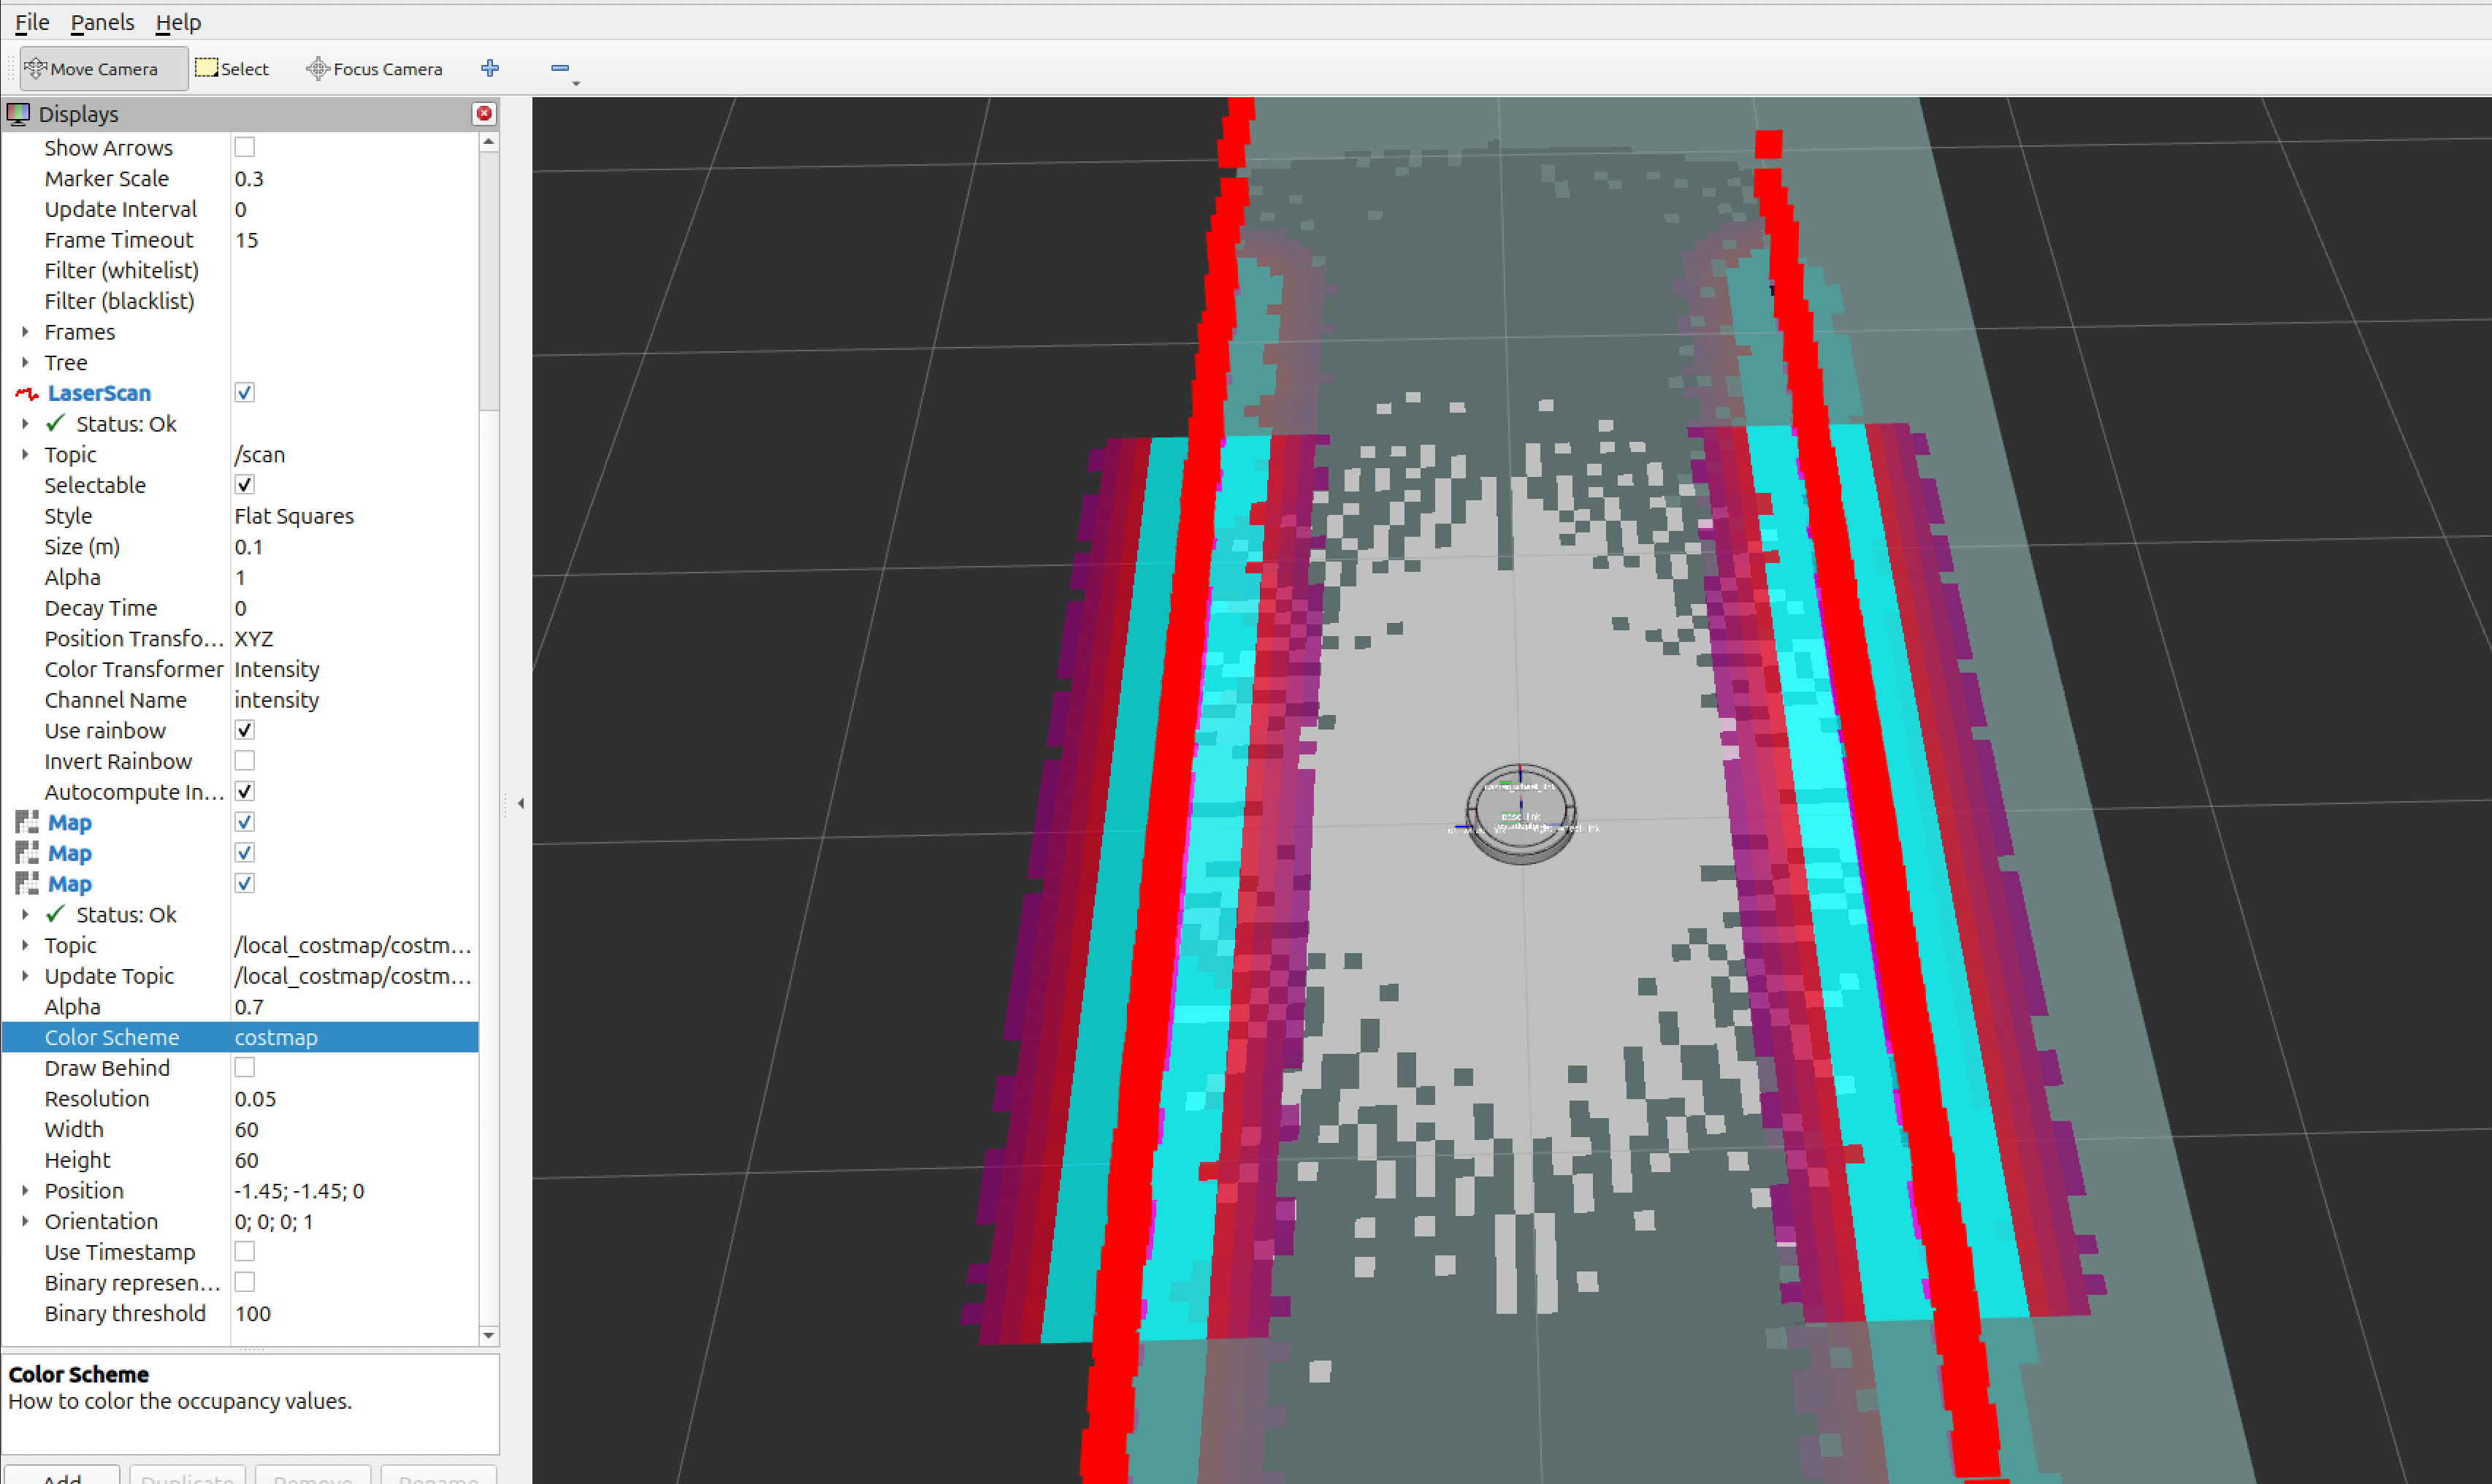
\includegraphics[width=\columnwidth]{fig/00_image.png}
    \caption{The global and local costmap around the robot. The grey path in
             the middle is free space.}
    \label{fig:costmap}
\end{figure}

We then sent the robot to goals with the 2D Goal Pose tool in RViz, as we can
see in Fig.~\ref{fig:goal1} to Fig.~\ref{fig:goal4}. The green line is the
path Nav2 planned to the goal. The map grows as the robot drives, since
\texttt{slam\_toolbox} keeps mapping while Nav2 drives.

\begin{figure}[H]
    \centering
    \begin{subfigure}{\columnwidth}
        \centering
        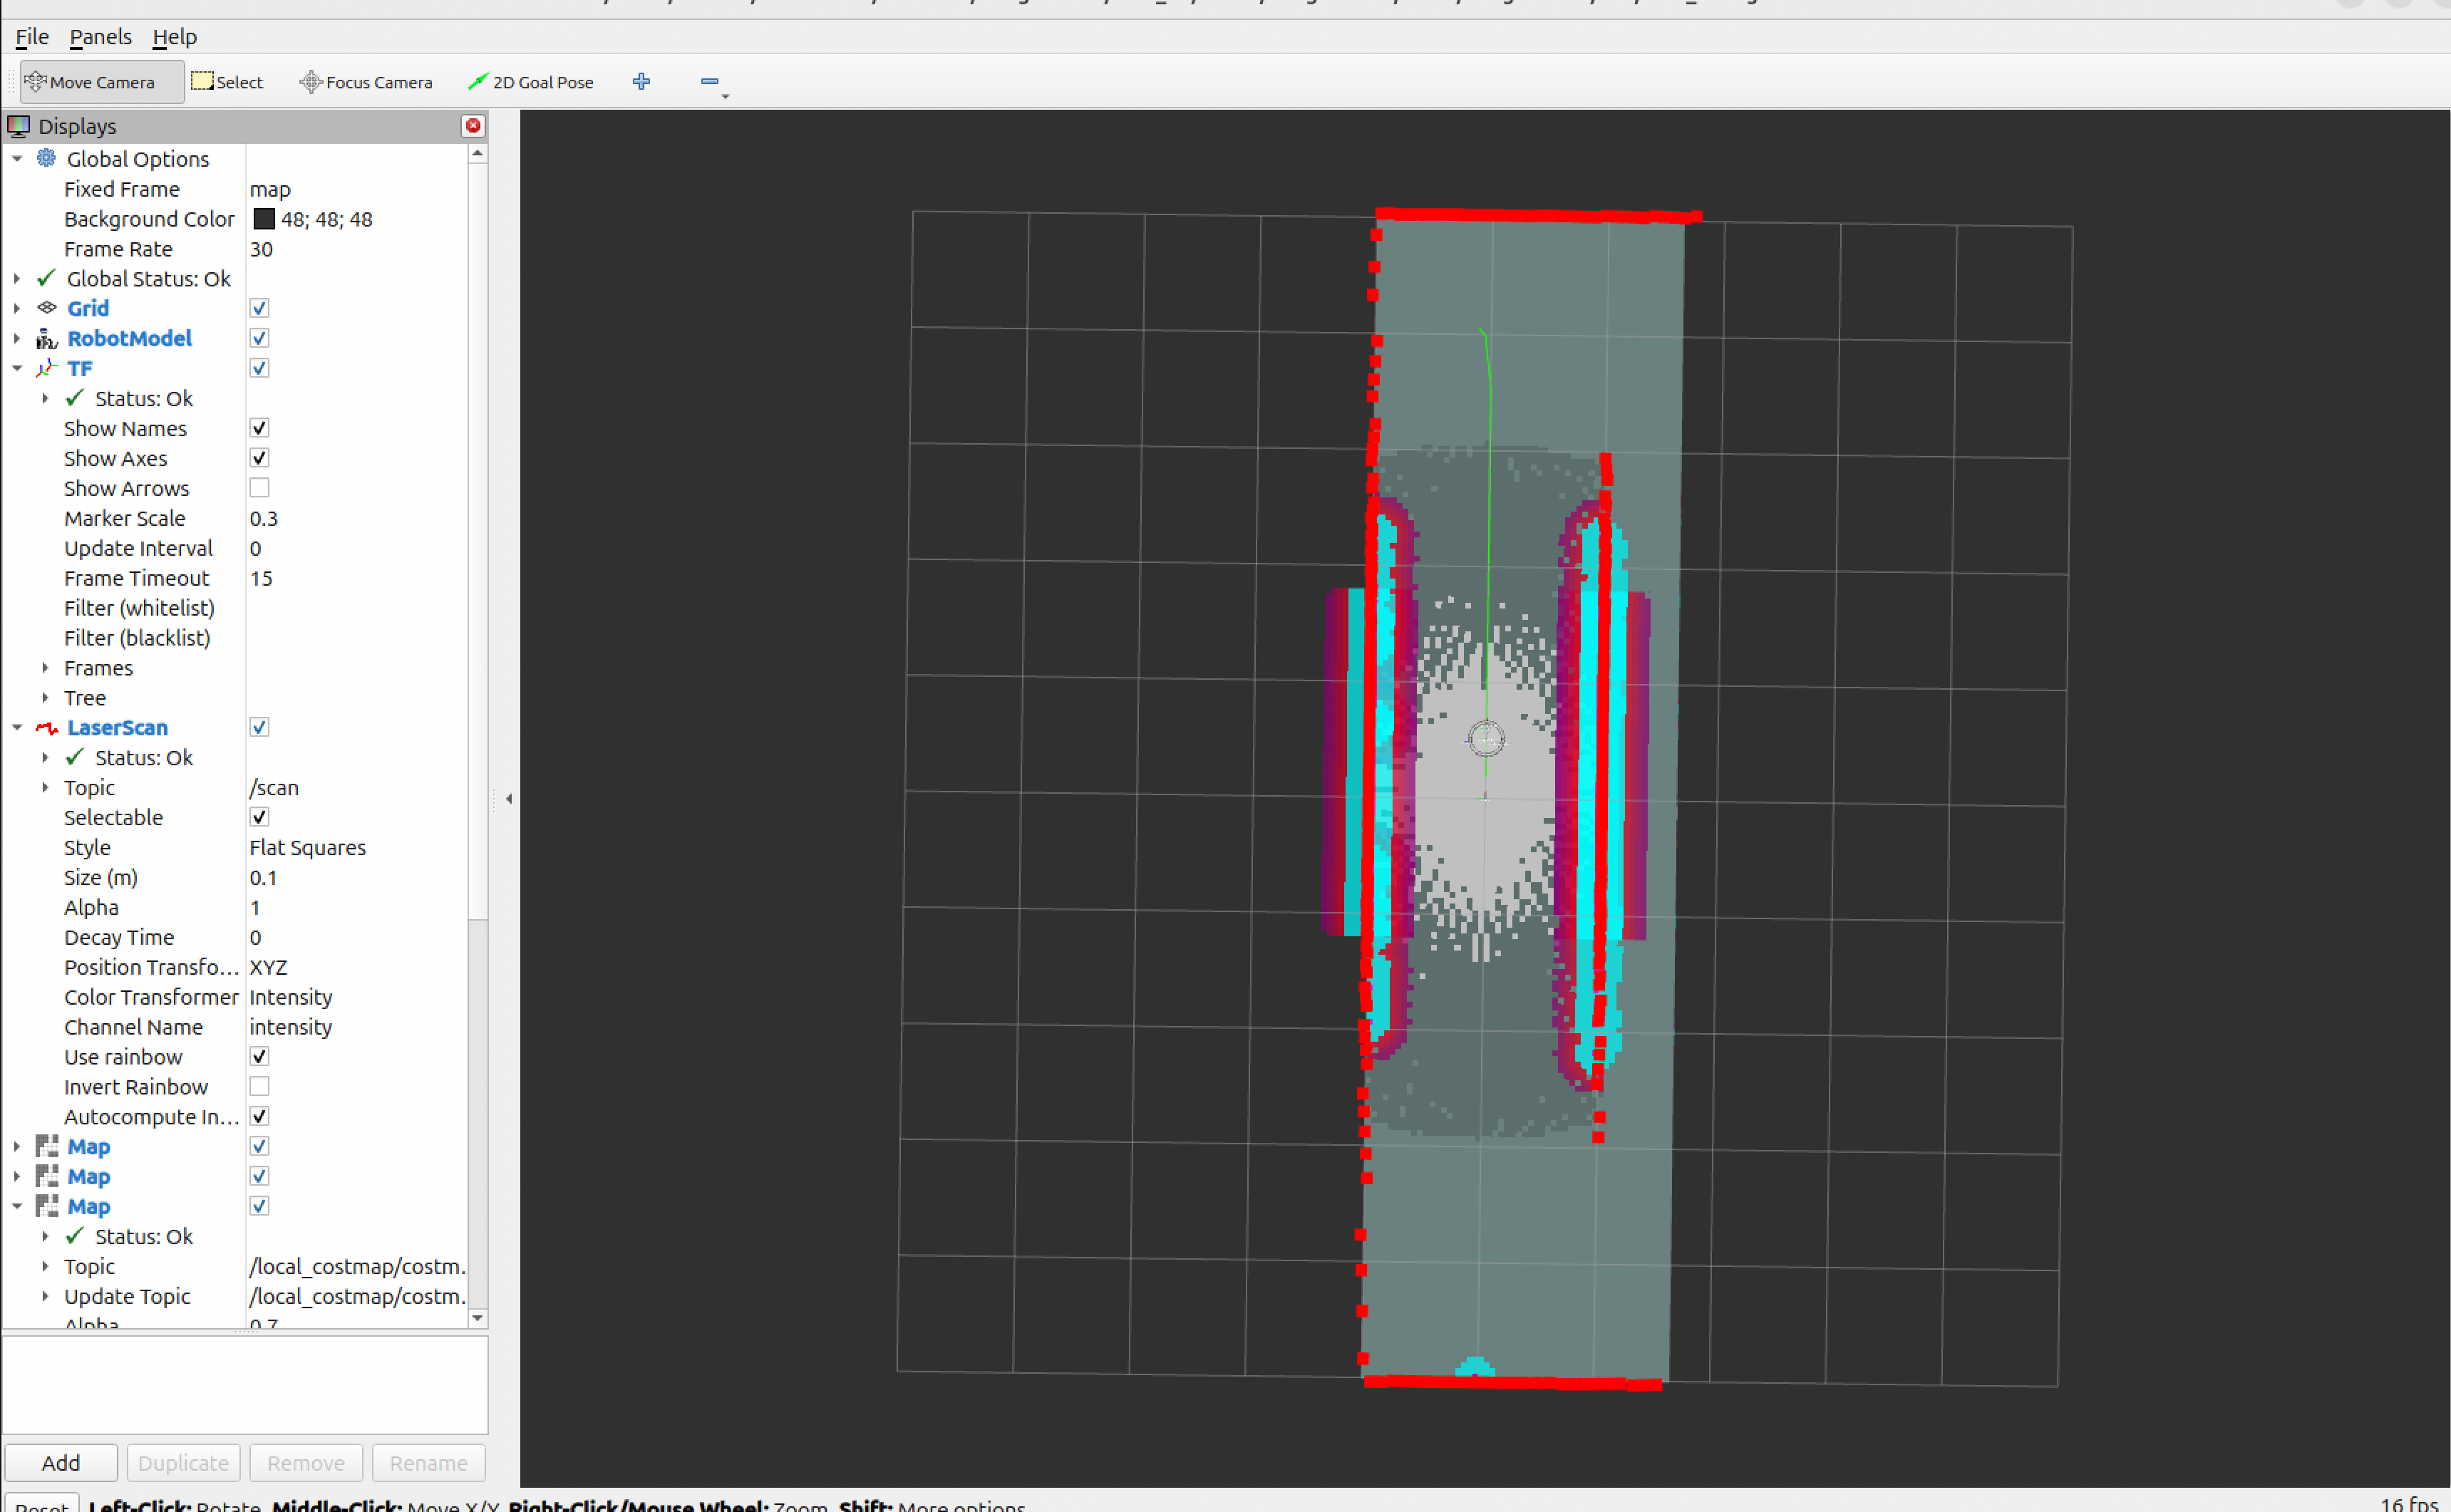
\includegraphics[width=\columnwidth]{fig/01_start.png}
        \caption{Start. The path goes straight up the corridor.}
    \end{subfigure}
    \begin{subfigure}{\columnwidth}
        \centering
        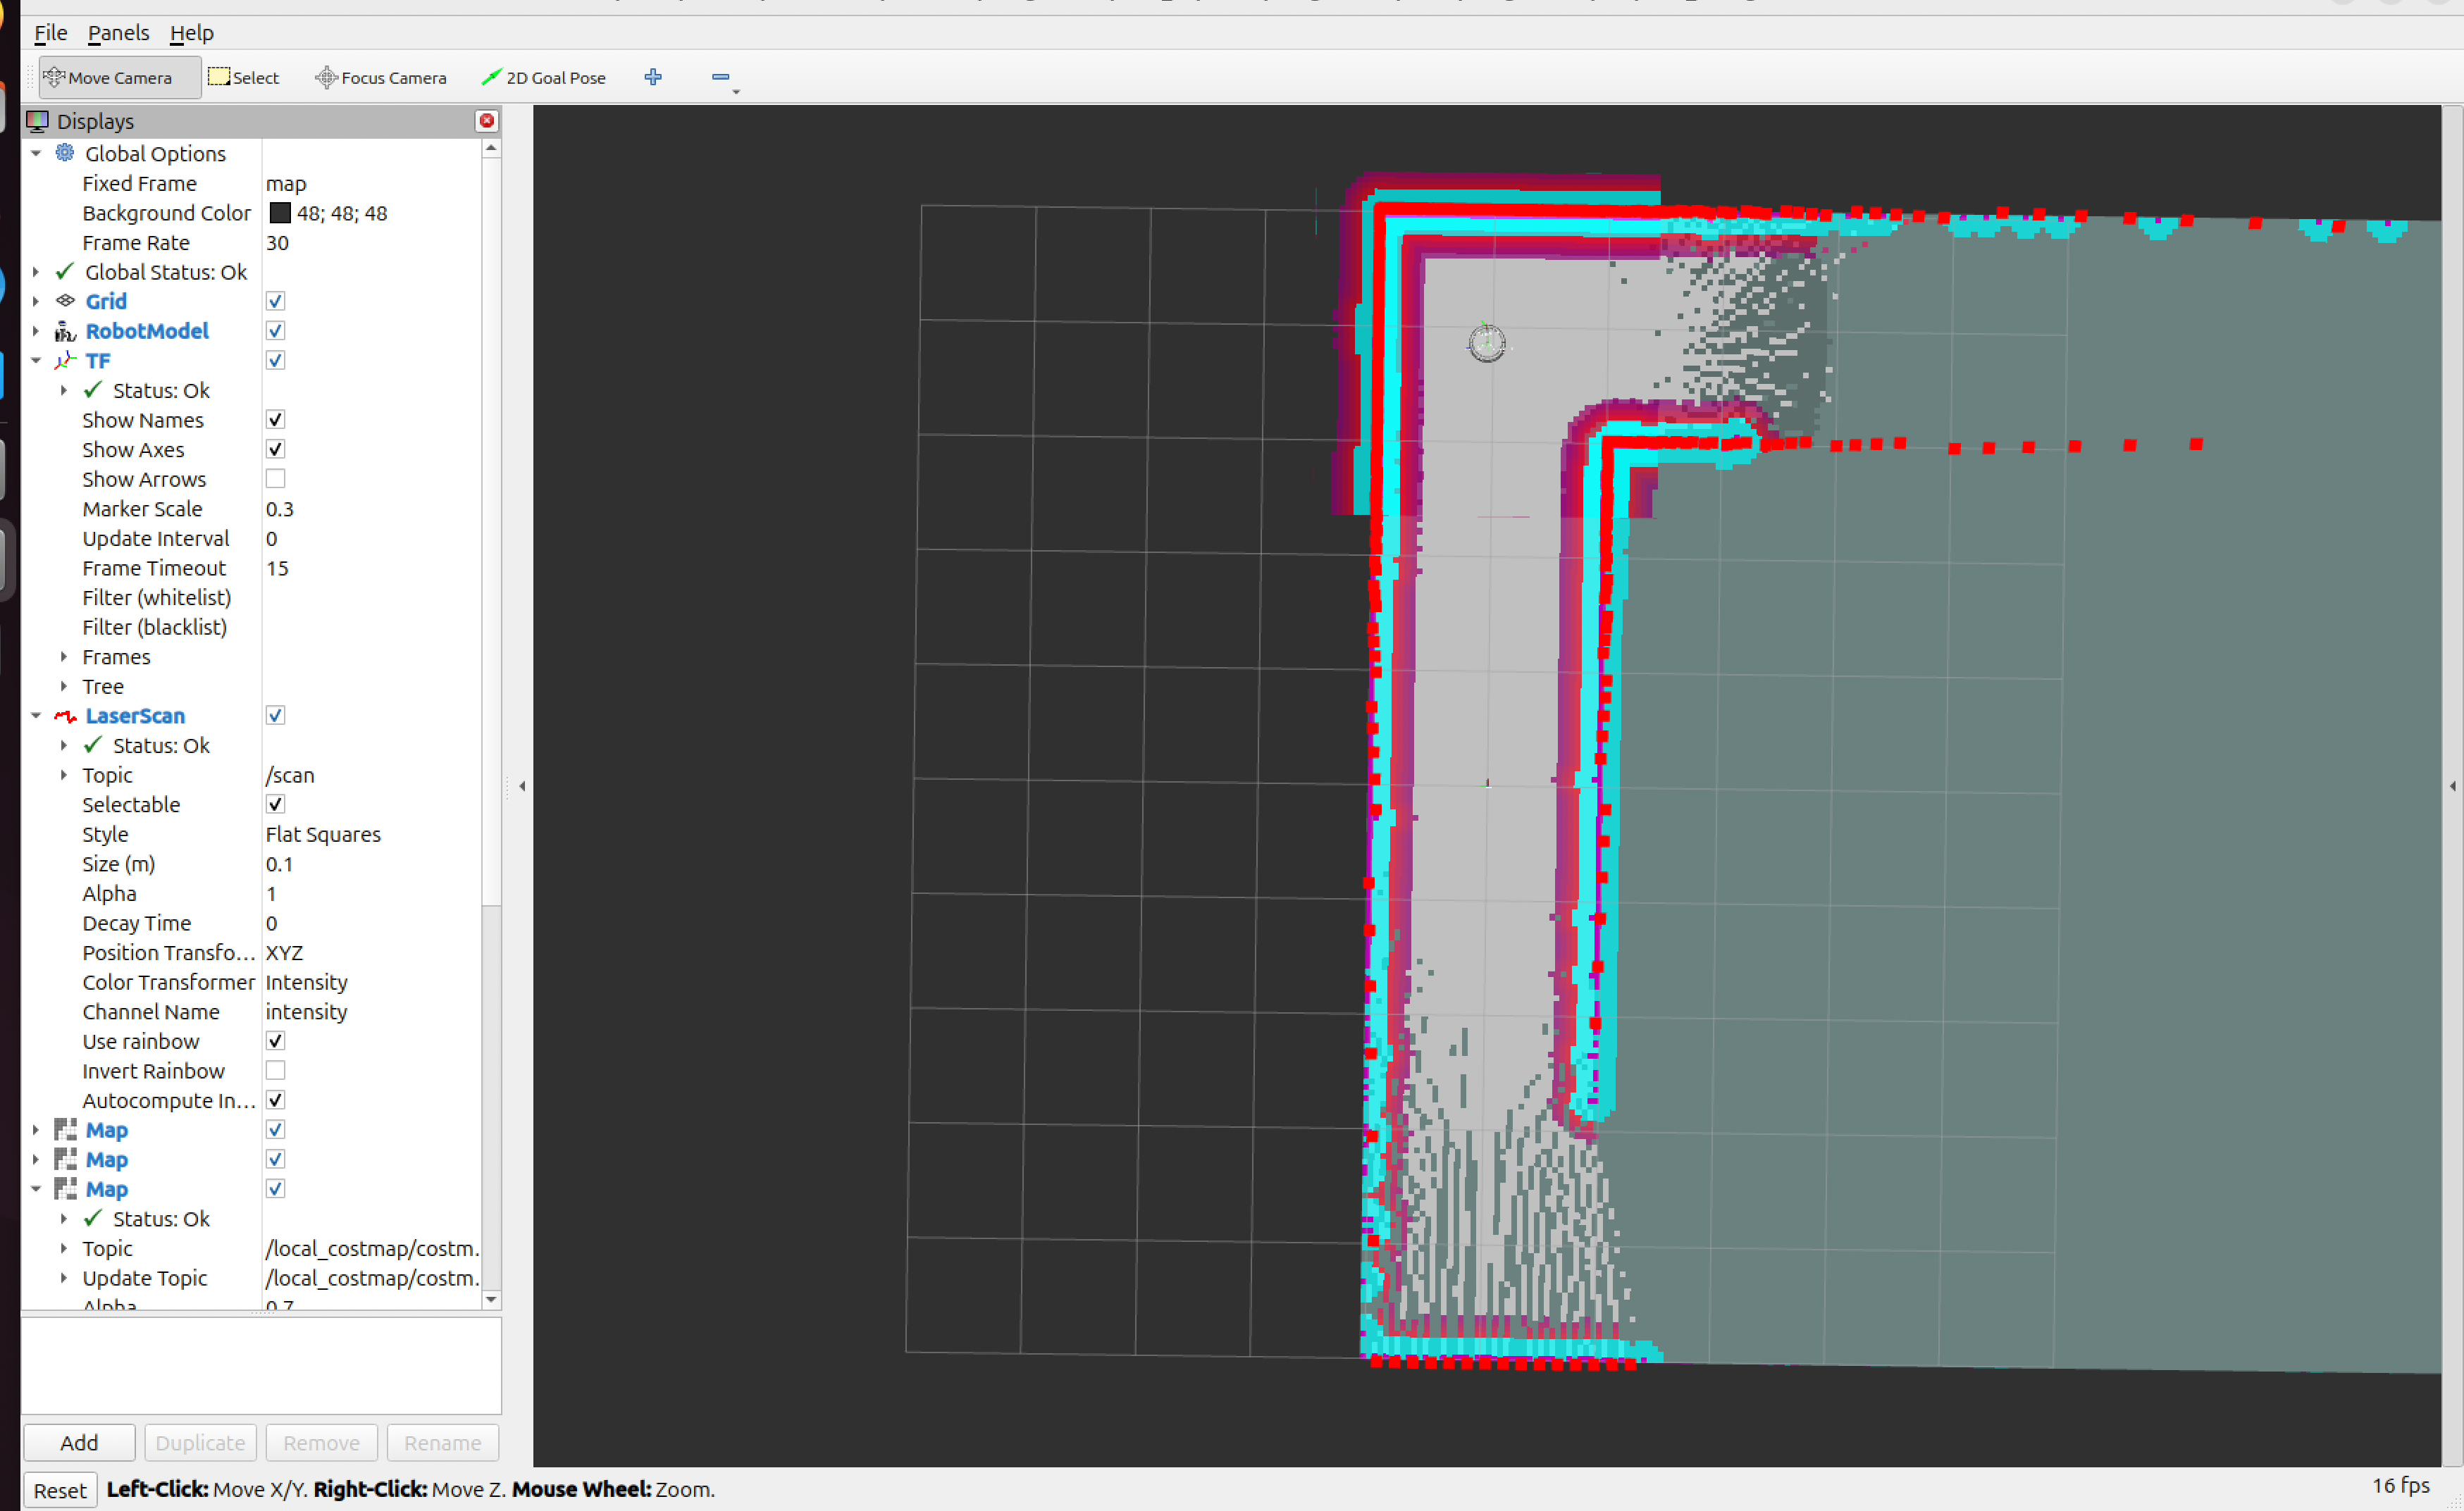
\includegraphics[width=\columnwidth]{fig/02_end.png}
        \caption{End. The robot has reached the goal and mapped the corner.}
    \end{subfigure}
    \caption{Goal 1, straight up the first corridor.}
    \label{fig:goal1}
\end{figure}

\begin{figure}[H]
    \centering
    \begin{subfigure}{\columnwidth}
        \centering
        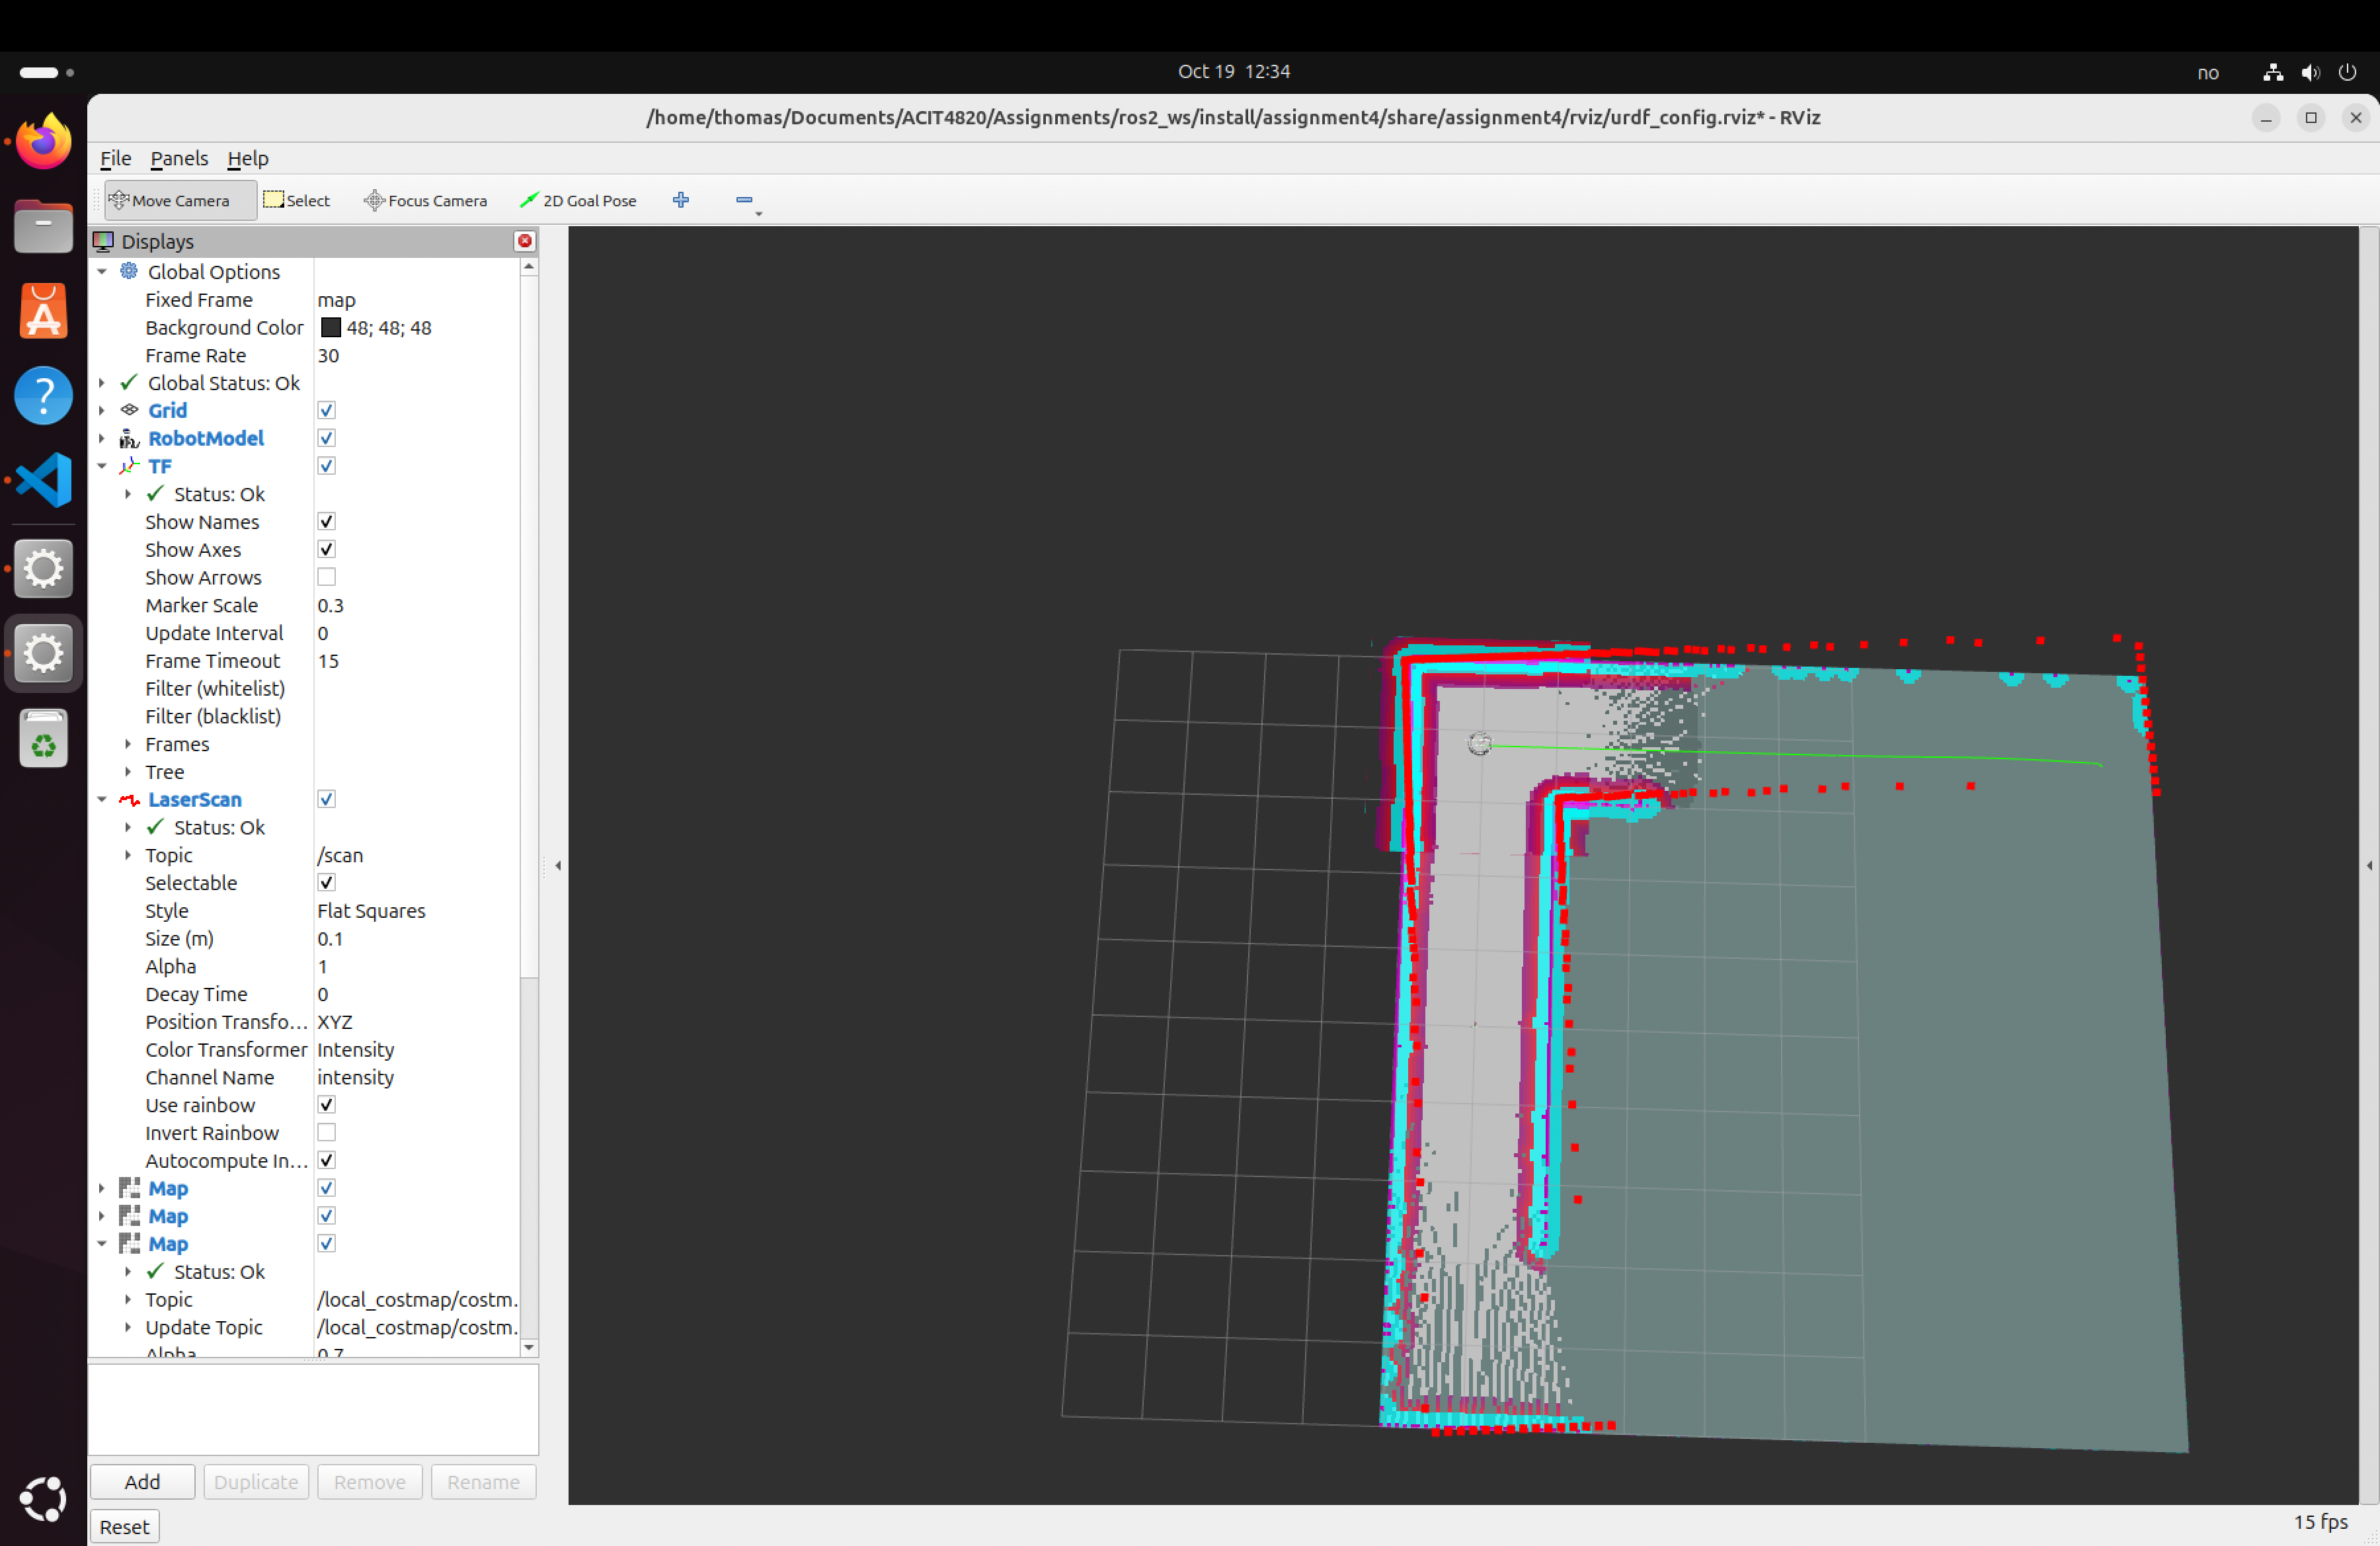
\includegraphics[width=\columnwidth]{fig/03_start.png}
        \caption{Start. The path goes around the corner.}
    \end{subfigure}
    \begin{subfigure}{\columnwidth}
        \centering
        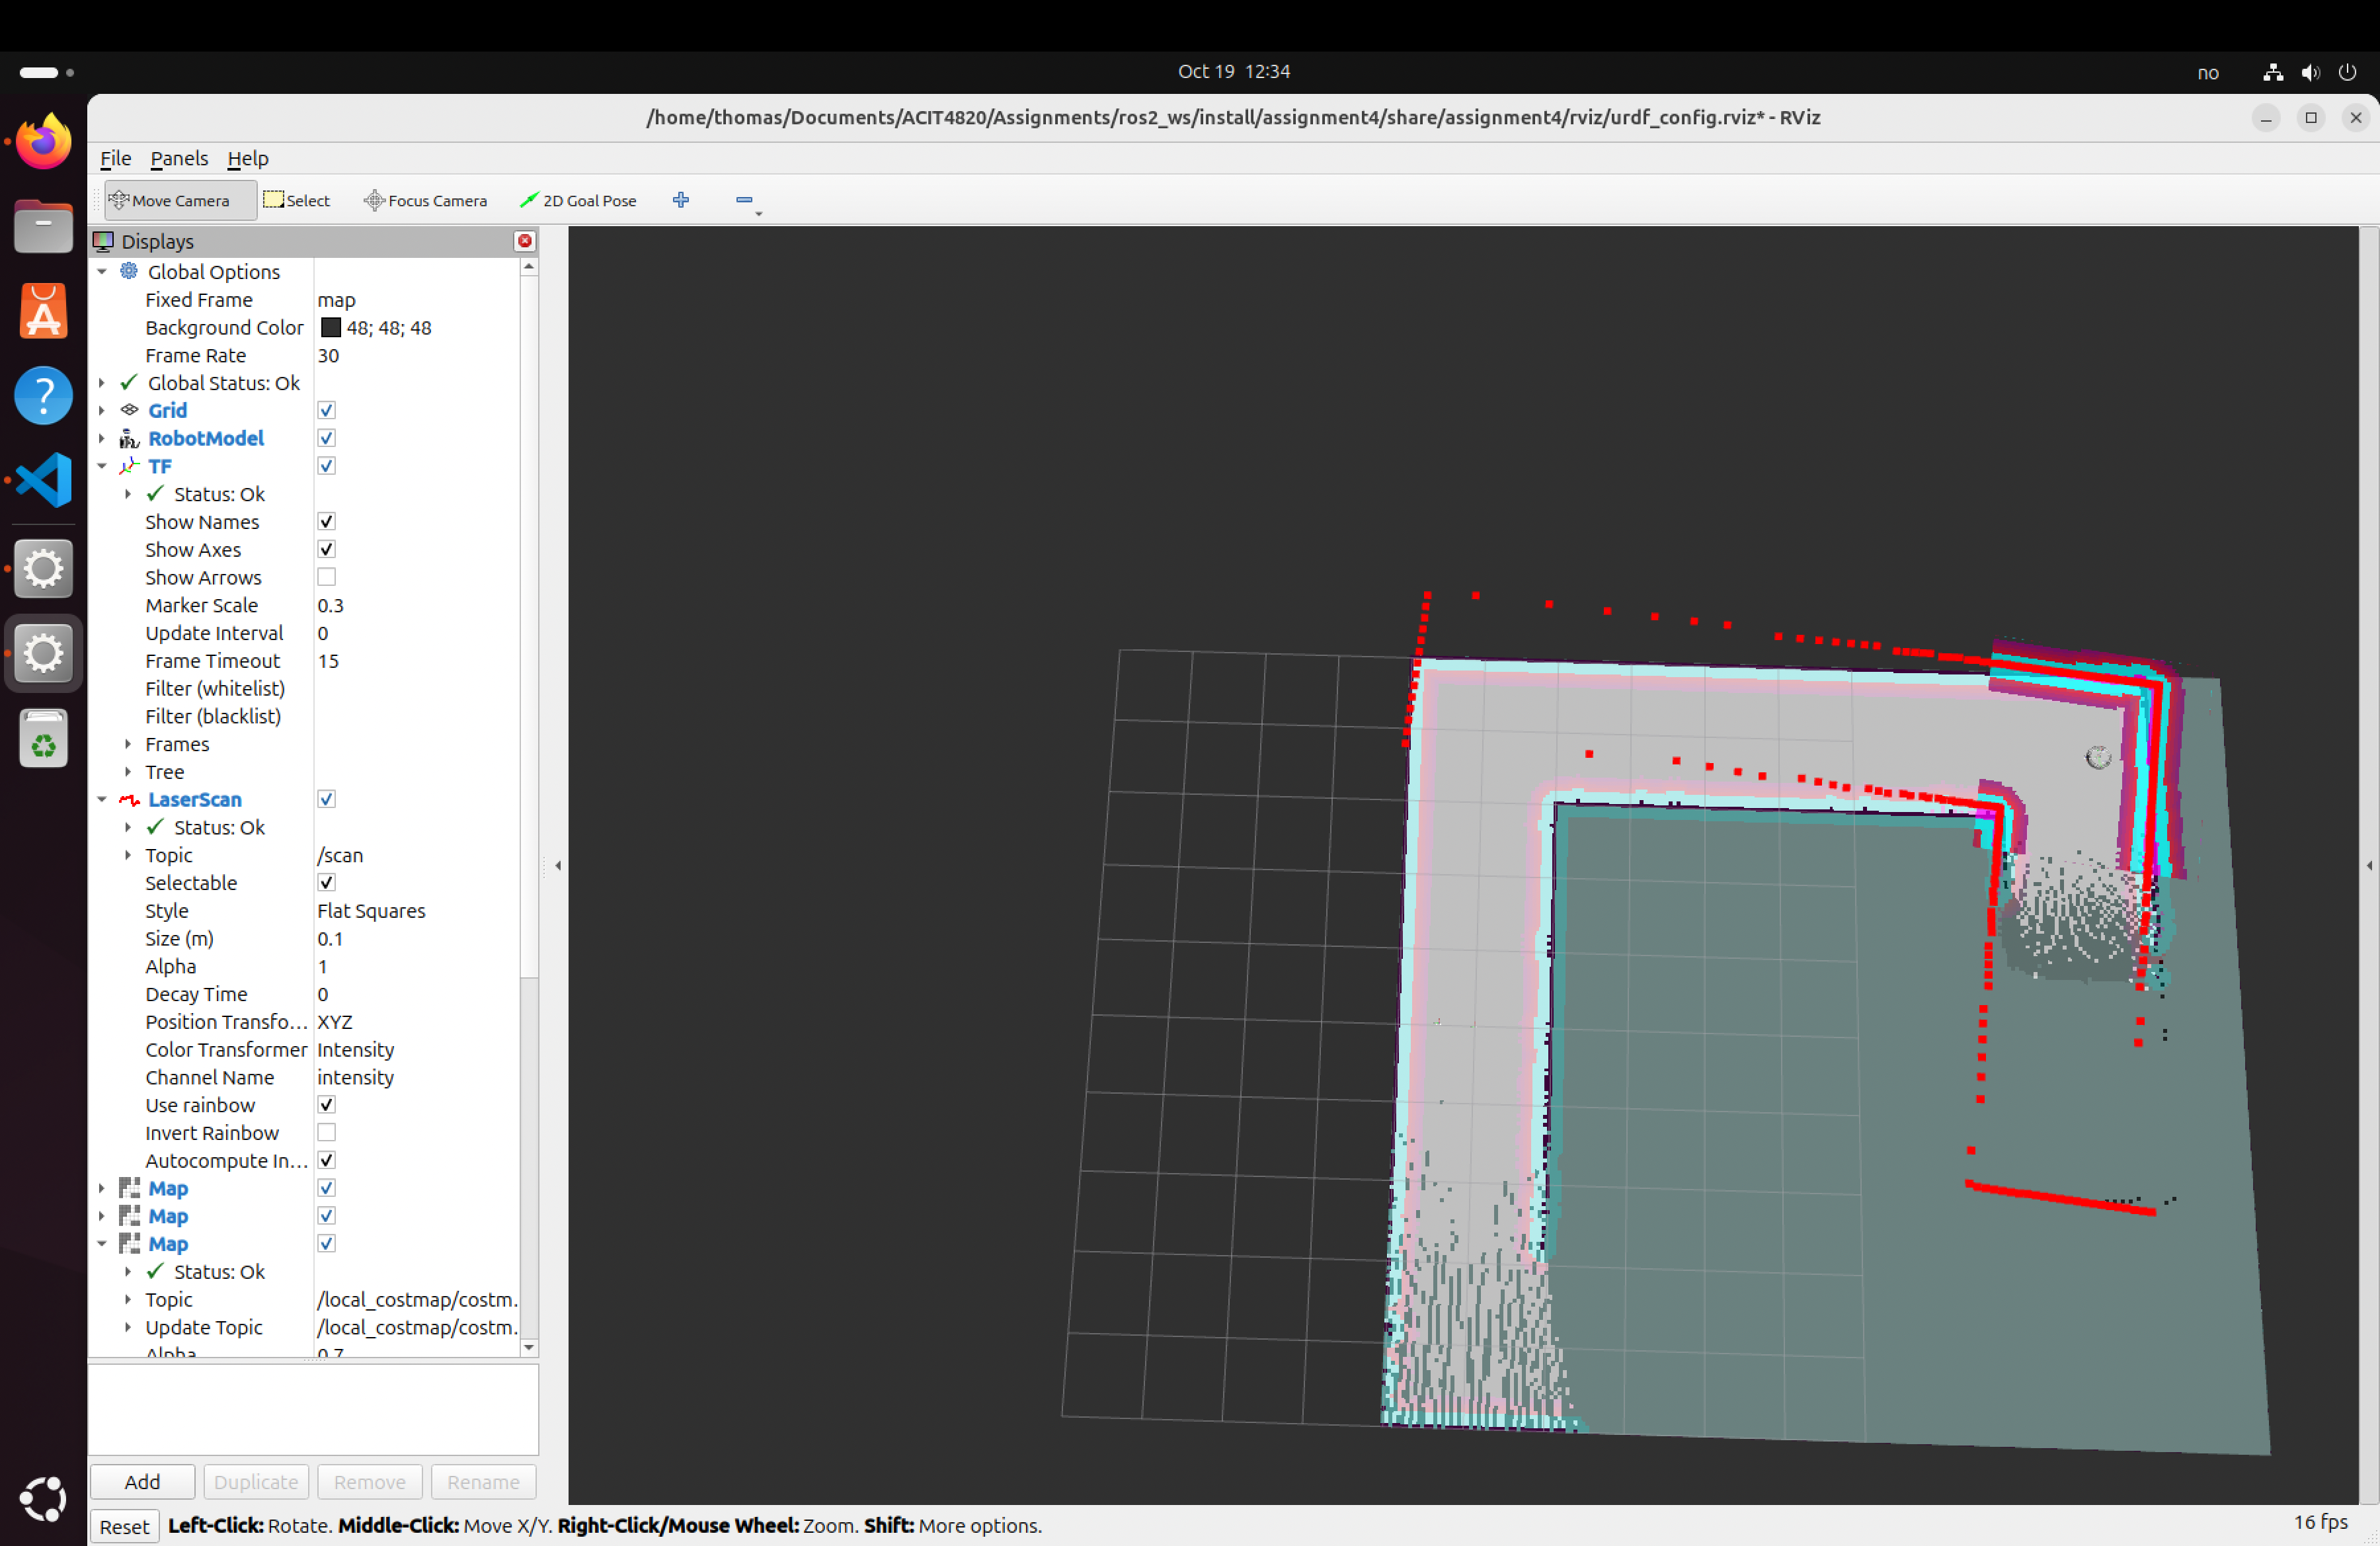
\includegraphics[width=\columnwidth]{fig/04_end.png}
        \caption{End. The top corridor is now mapped.}
    \end{subfigure}
    \caption{Goal 2, around the first corner.}
    \label{fig:goal2}
\end{figure}

\begin{figure}[H]
    \centering
    \begin{subfigure}{\columnwidth}
        \centering
        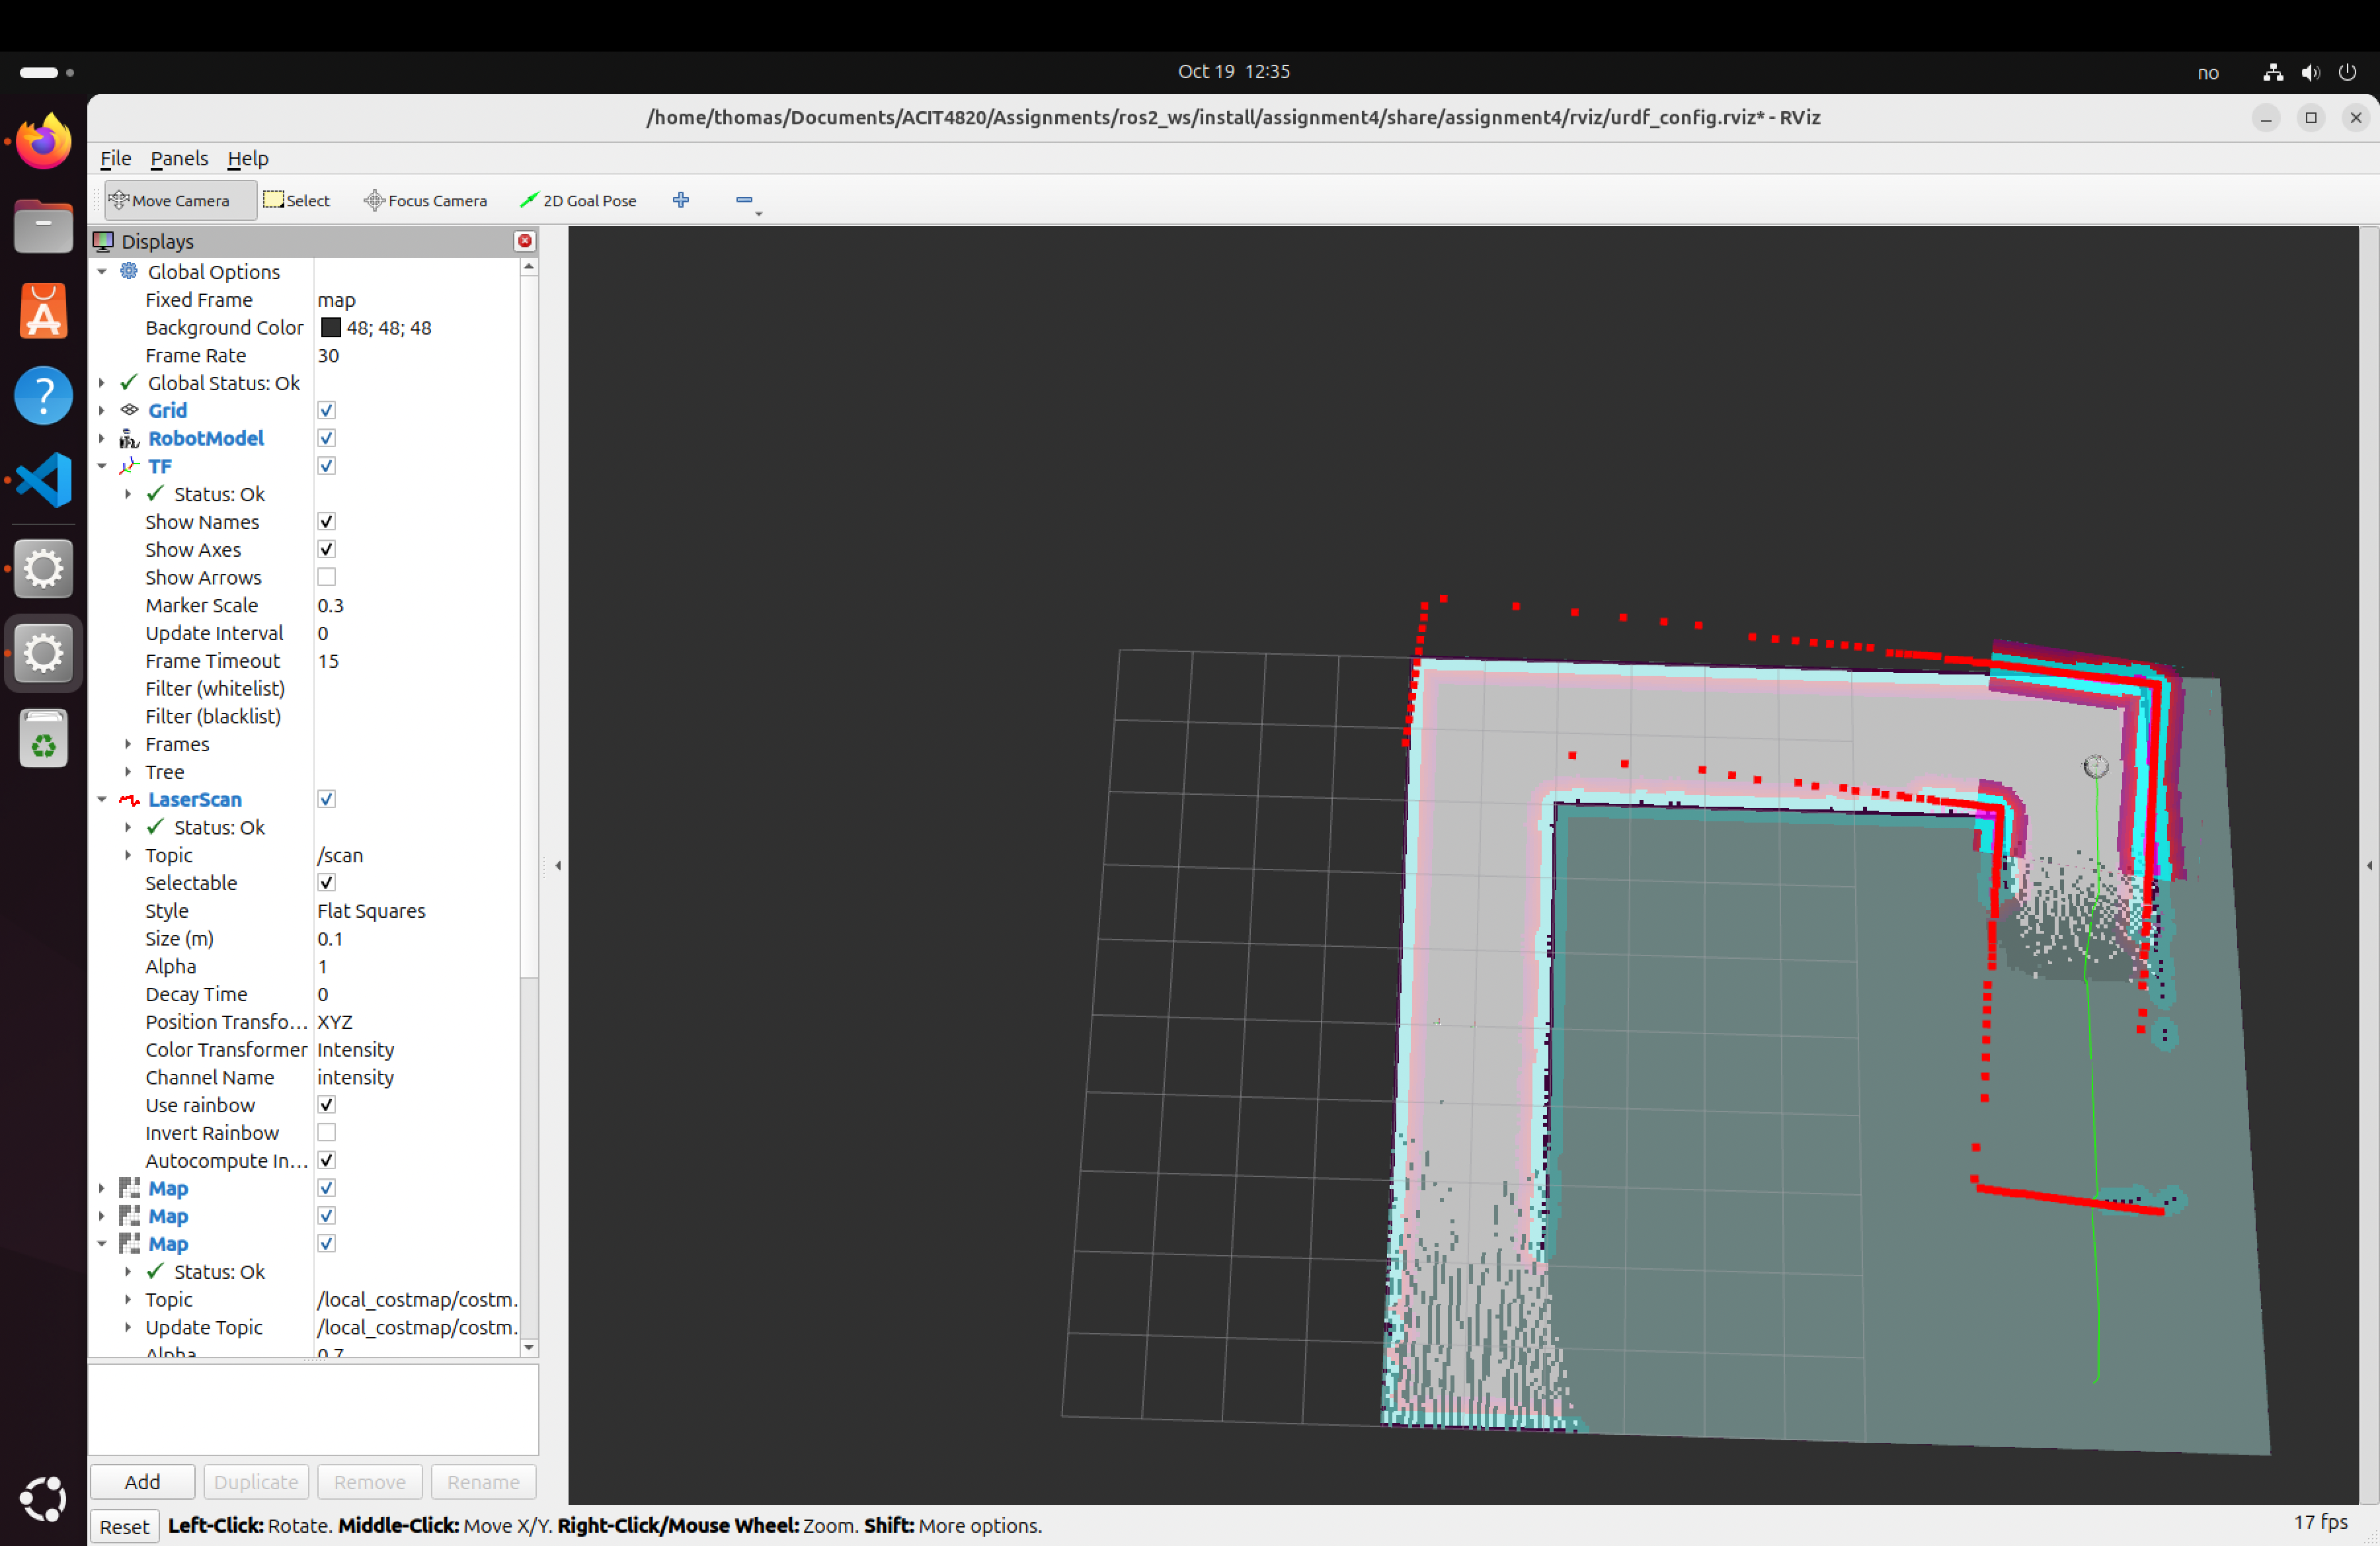
\includegraphics[width=\columnwidth]{fig/05_start.png}
        \caption{Start. The path goes down the right corridor.}
    \end{subfigure}
    \begin{subfigure}{\columnwidth}
        \centering
        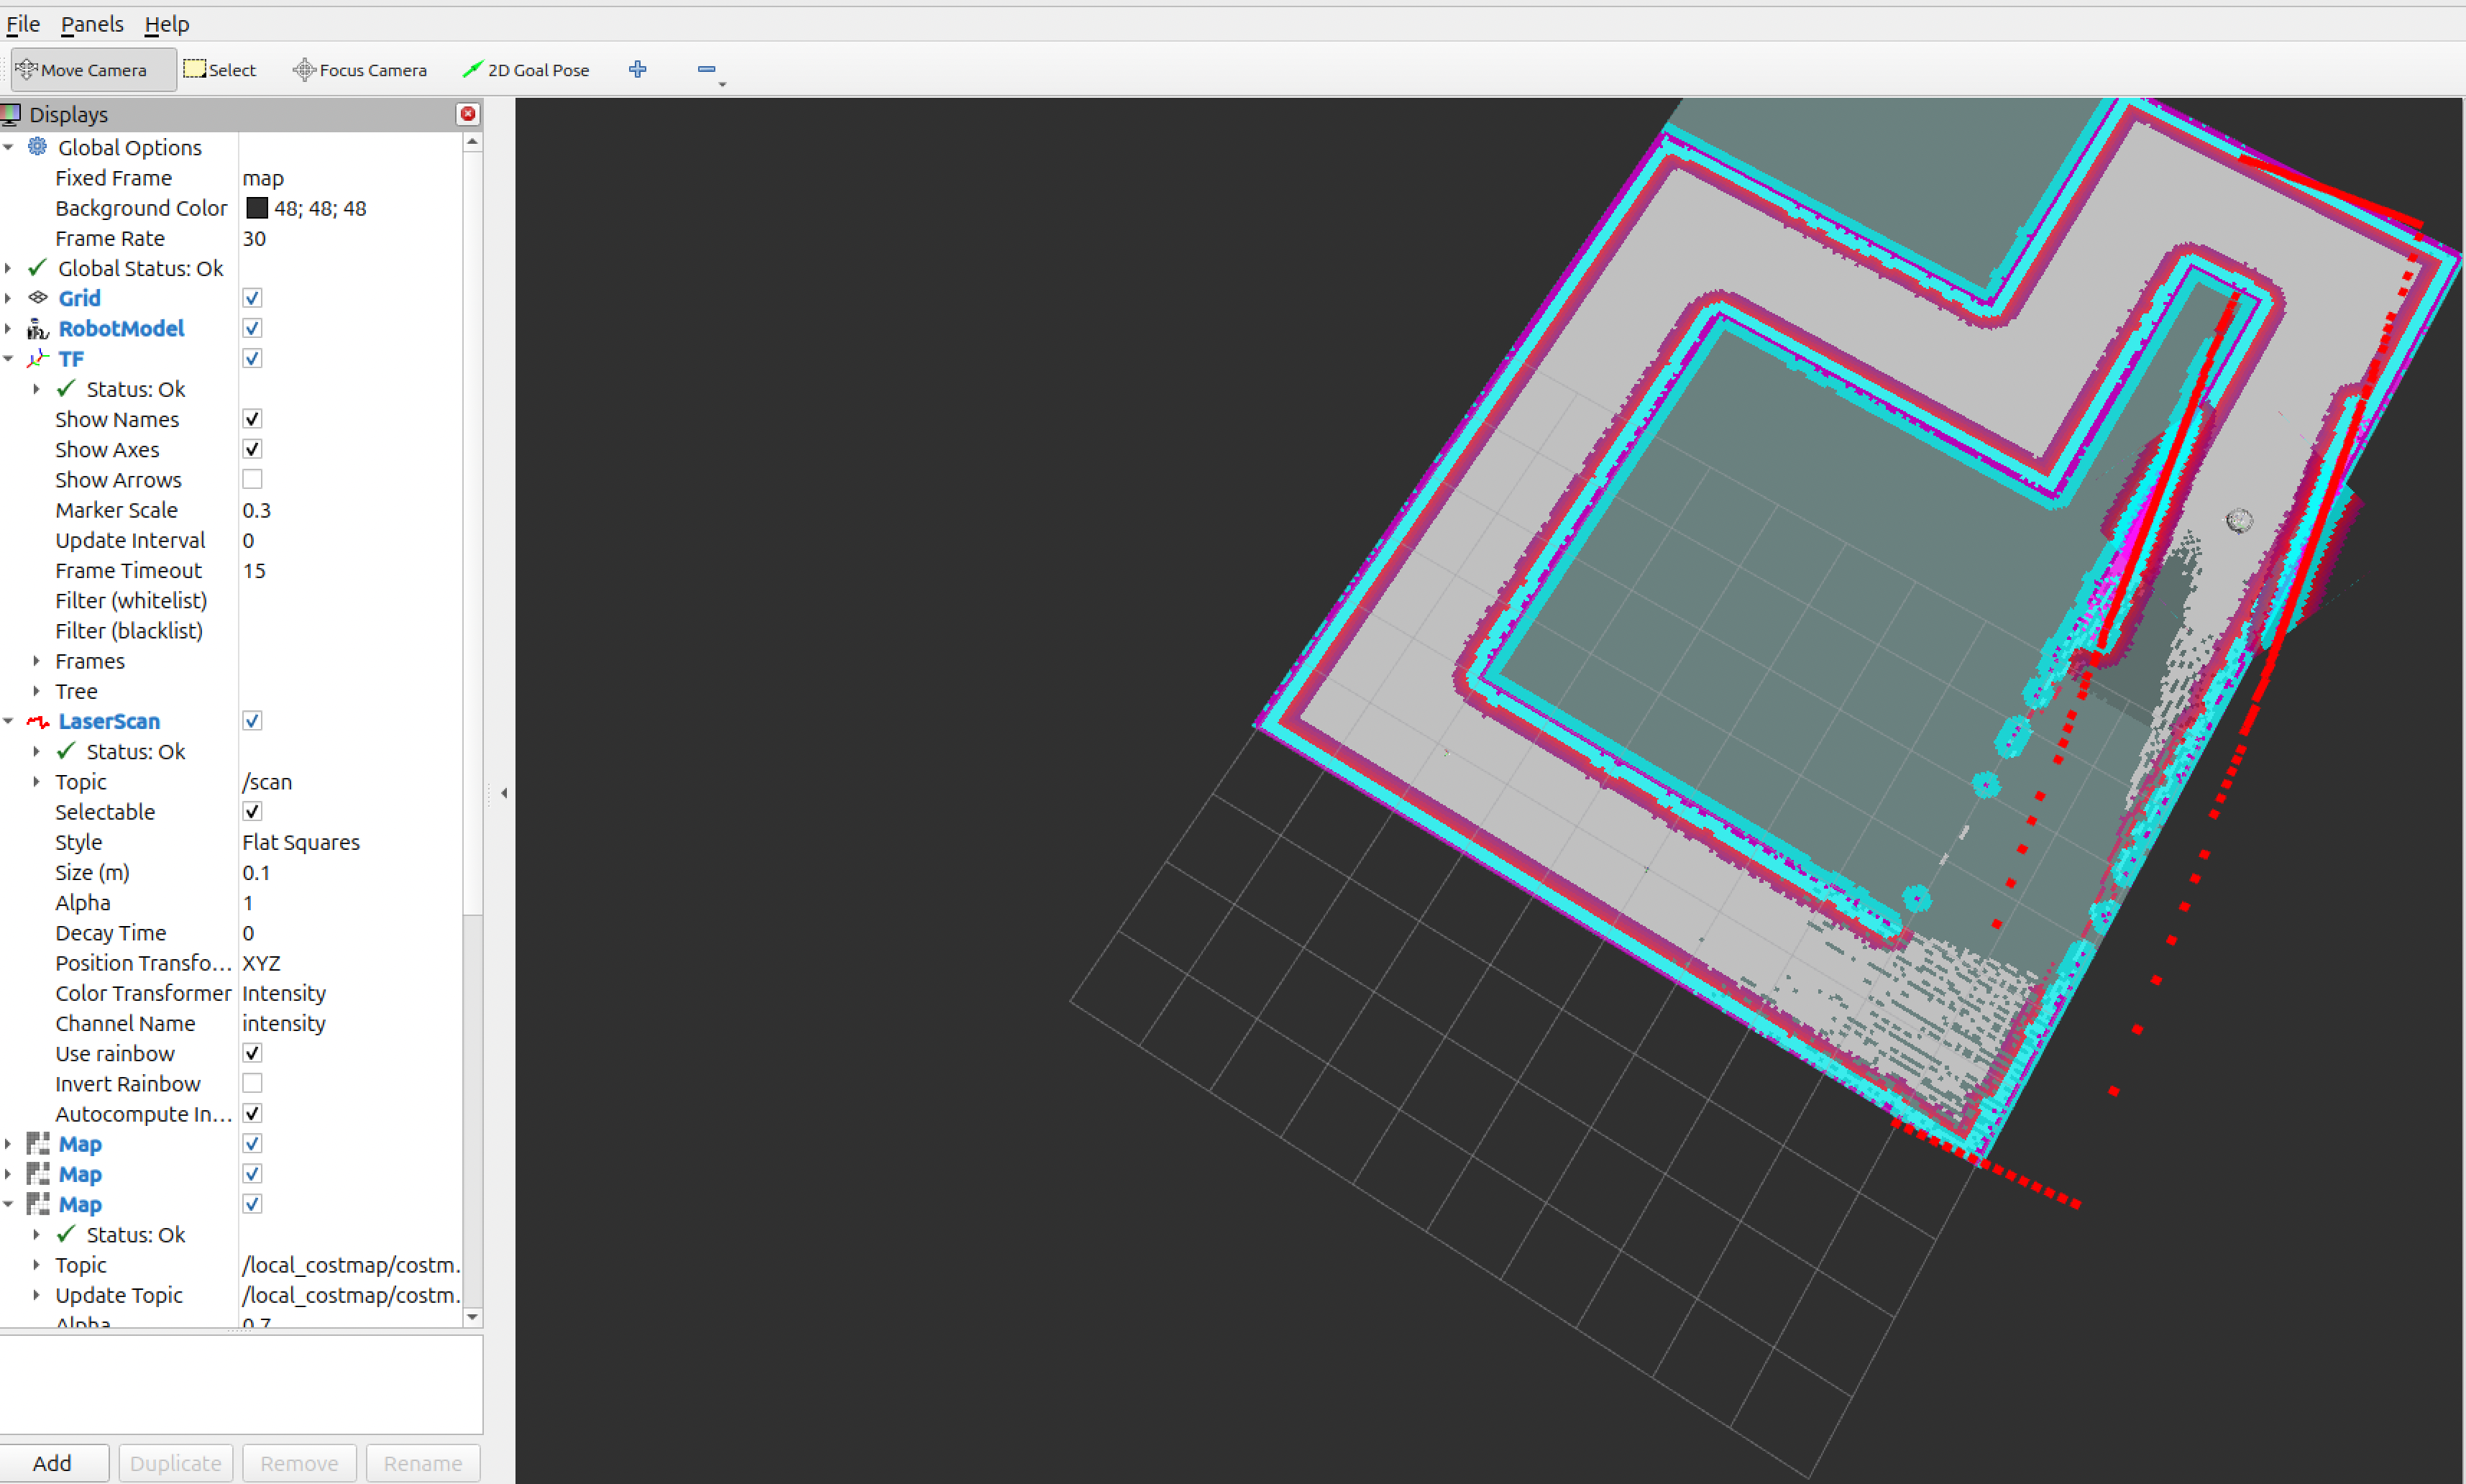
\includegraphics[width=\columnwidth]{fig/06_end.png}
        \caption{End. The walls on the right side are drawn twice.}
    \end{subfigure}
    \caption{Goal 3, down the right corridor.}
    \label{fig:goal3}
\end{figure}

\begin{figure}[H]
    \centering
    \begin{subfigure}{\columnwidth}
        \centering
        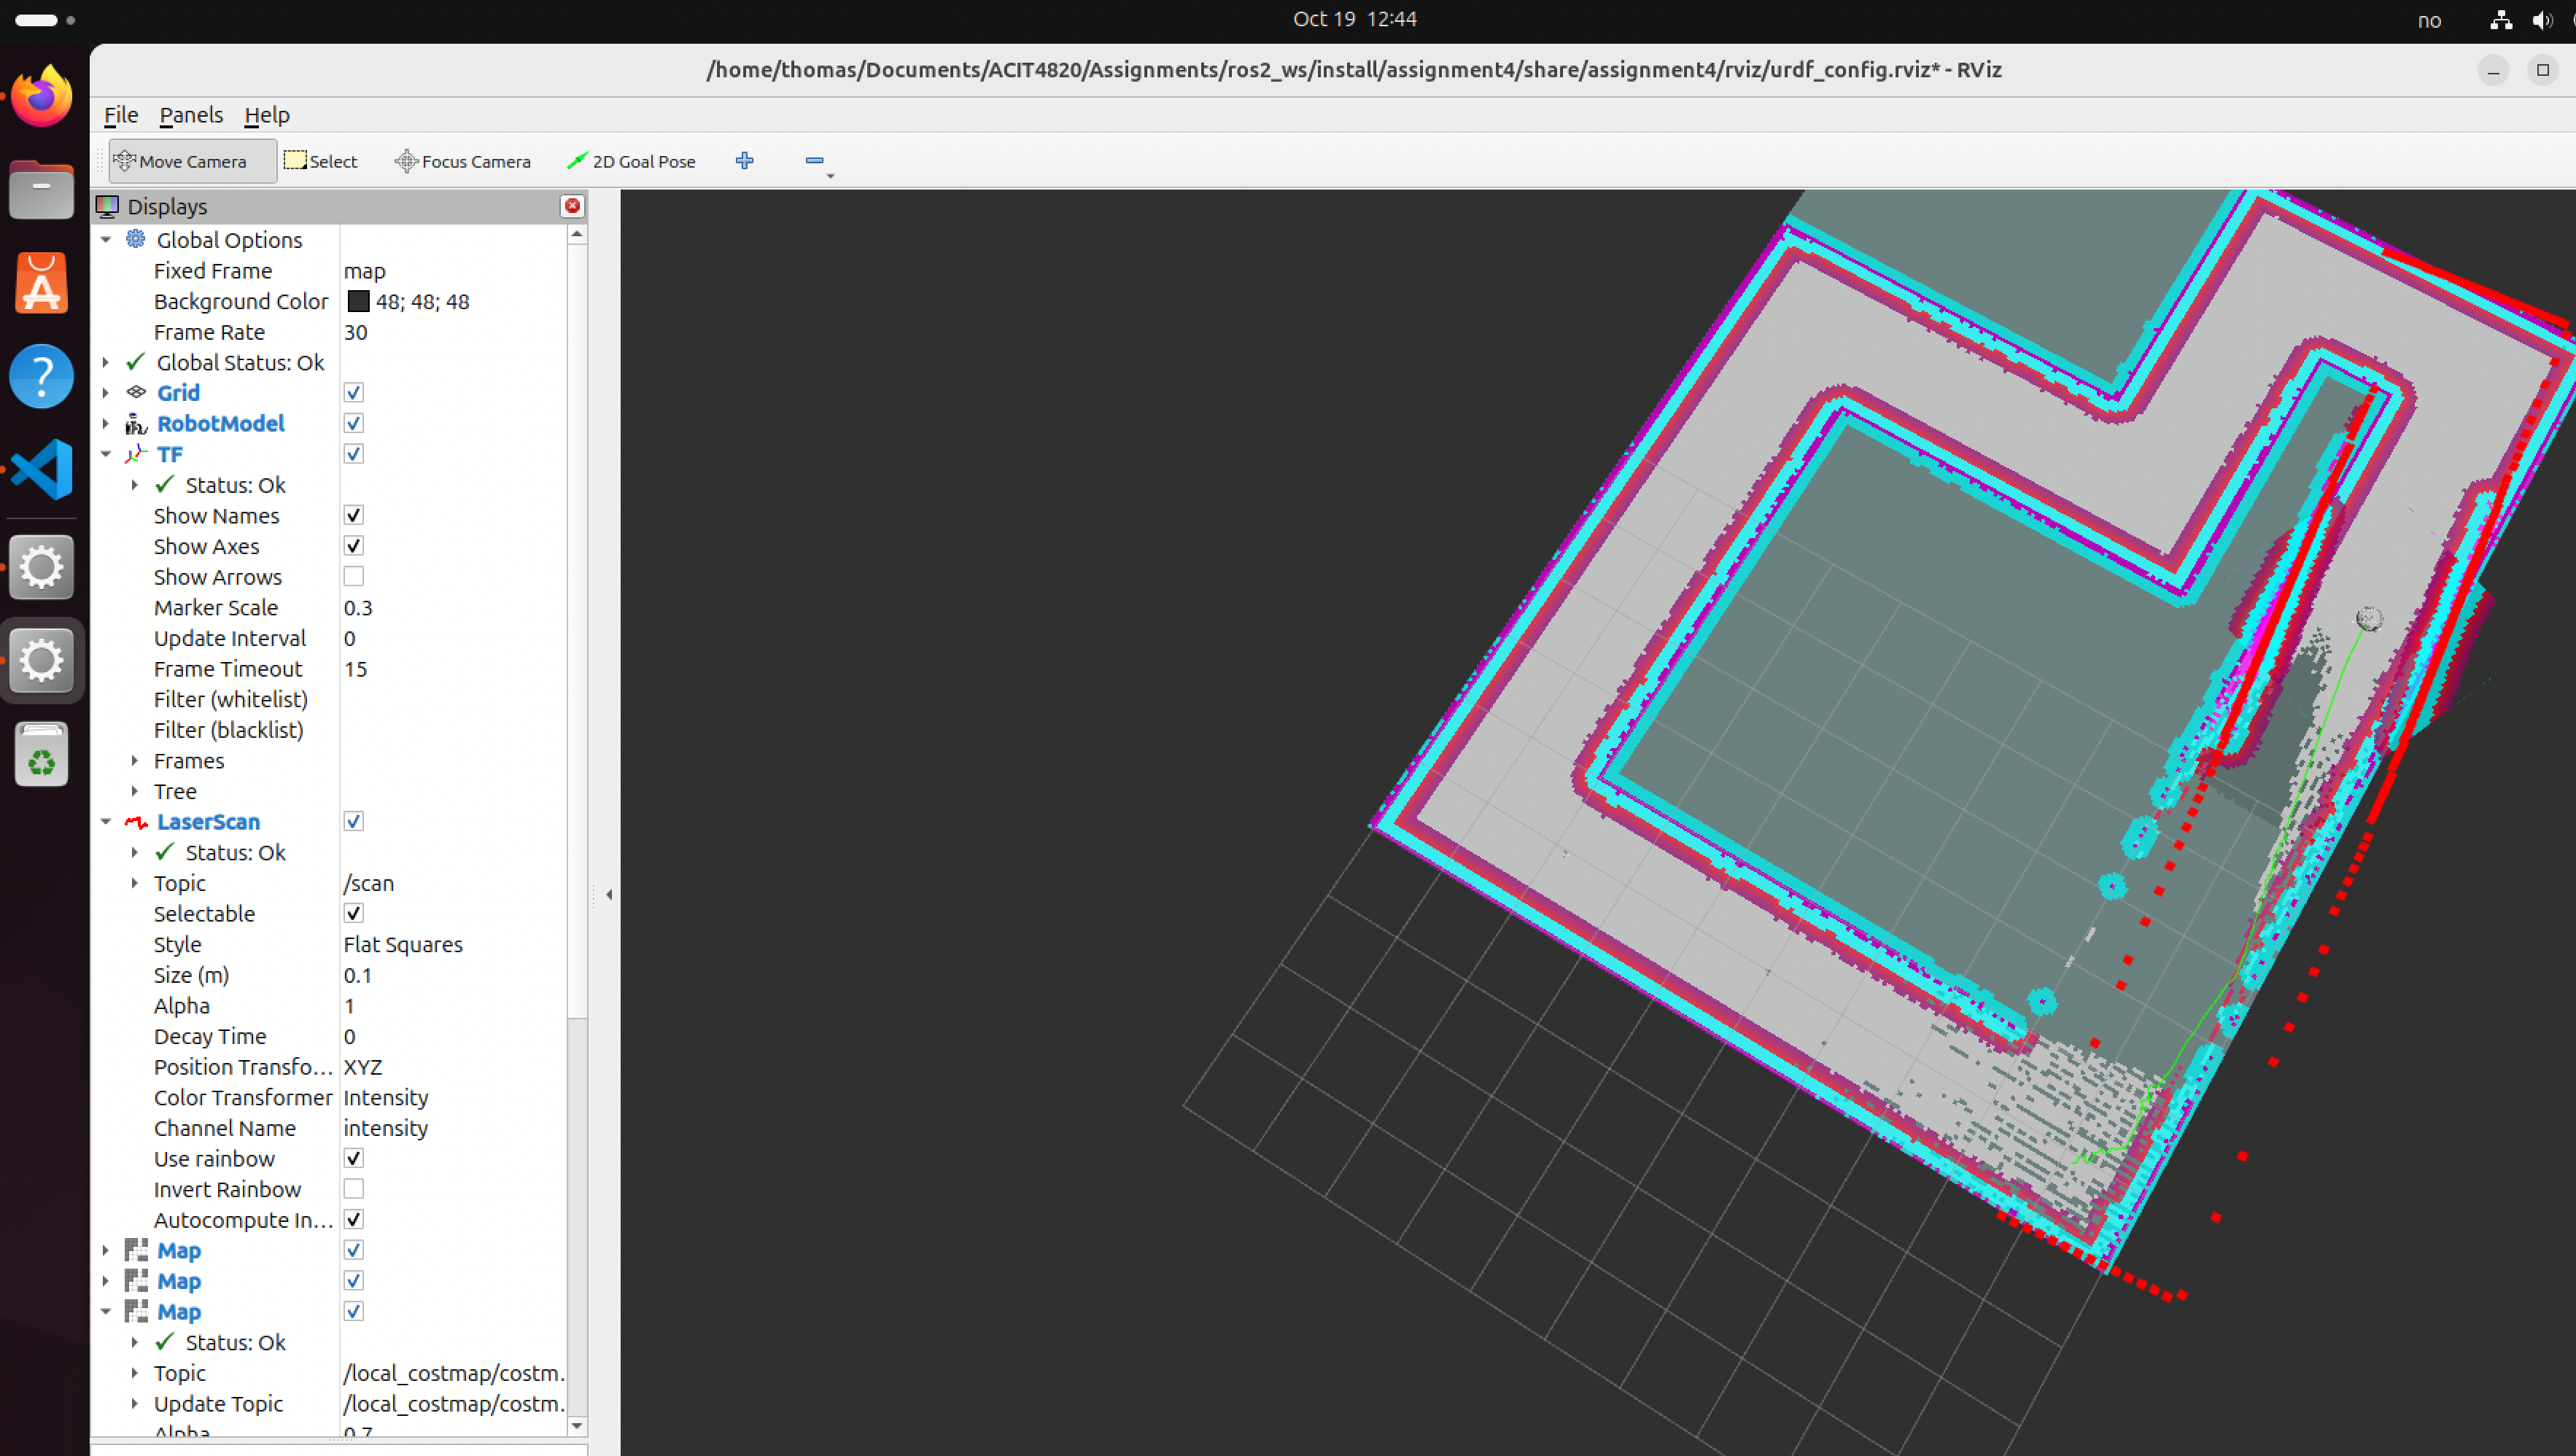
\includegraphics[width=\columnwidth]{fig/07_start.png}
        \caption{Start. The path follows the right corridor back down.}
    \end{subfigure}
    \begin{subfigure}{\columnwidth}
        \centering
        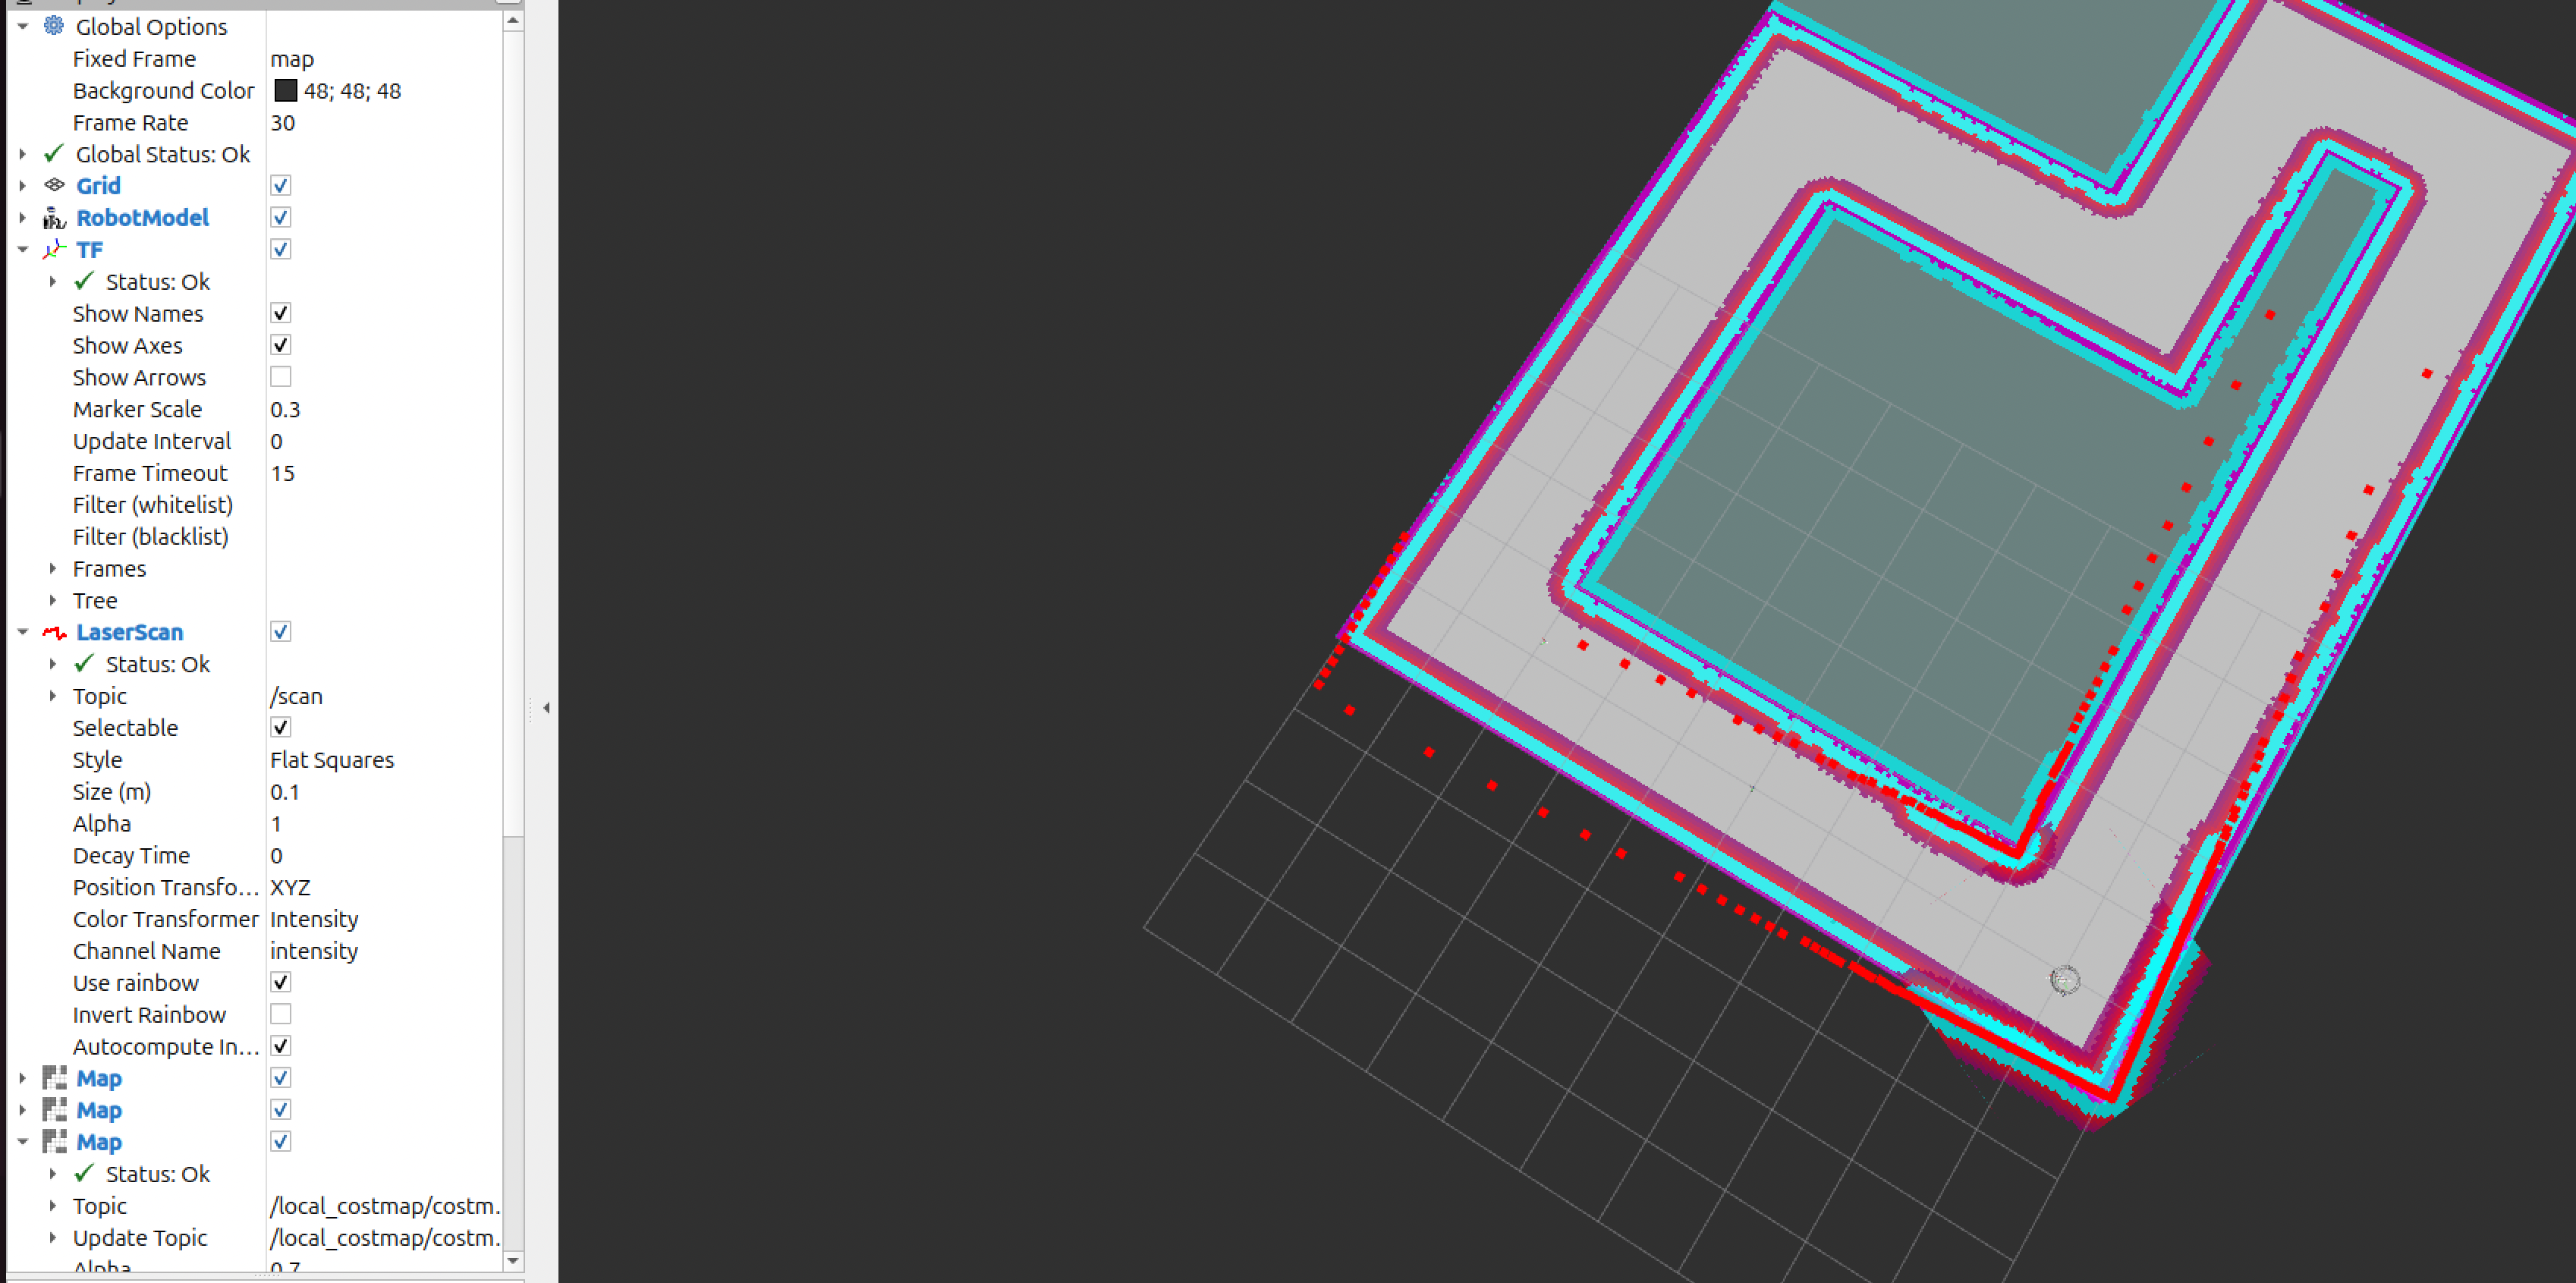
\includegraphics[width=\columnwidth]{fig/08_end.png}
        \caption{End. Most of the maze is mapped, but the scan on the right
                 does not line up with the map.}
    \end{subfigure}
    \caption{Goal 4, back along the right side of the maze.}
    \label{fig:goal4}
\end{figure}

\subsection{Task 3}
We started the launch file with \texttt{explore:=true} and let the robot drive
on its own. Fig.~\ref{fig:explore1} and Fig.~\ref{fig:explore2} show the
exploration from start to end. We did not send any goals. The green line is
the path to the frontier the explorer chose.

\begin{figure}[H]
    \centering
    \begin{subfigure}{\columnwidth}
        \centering
        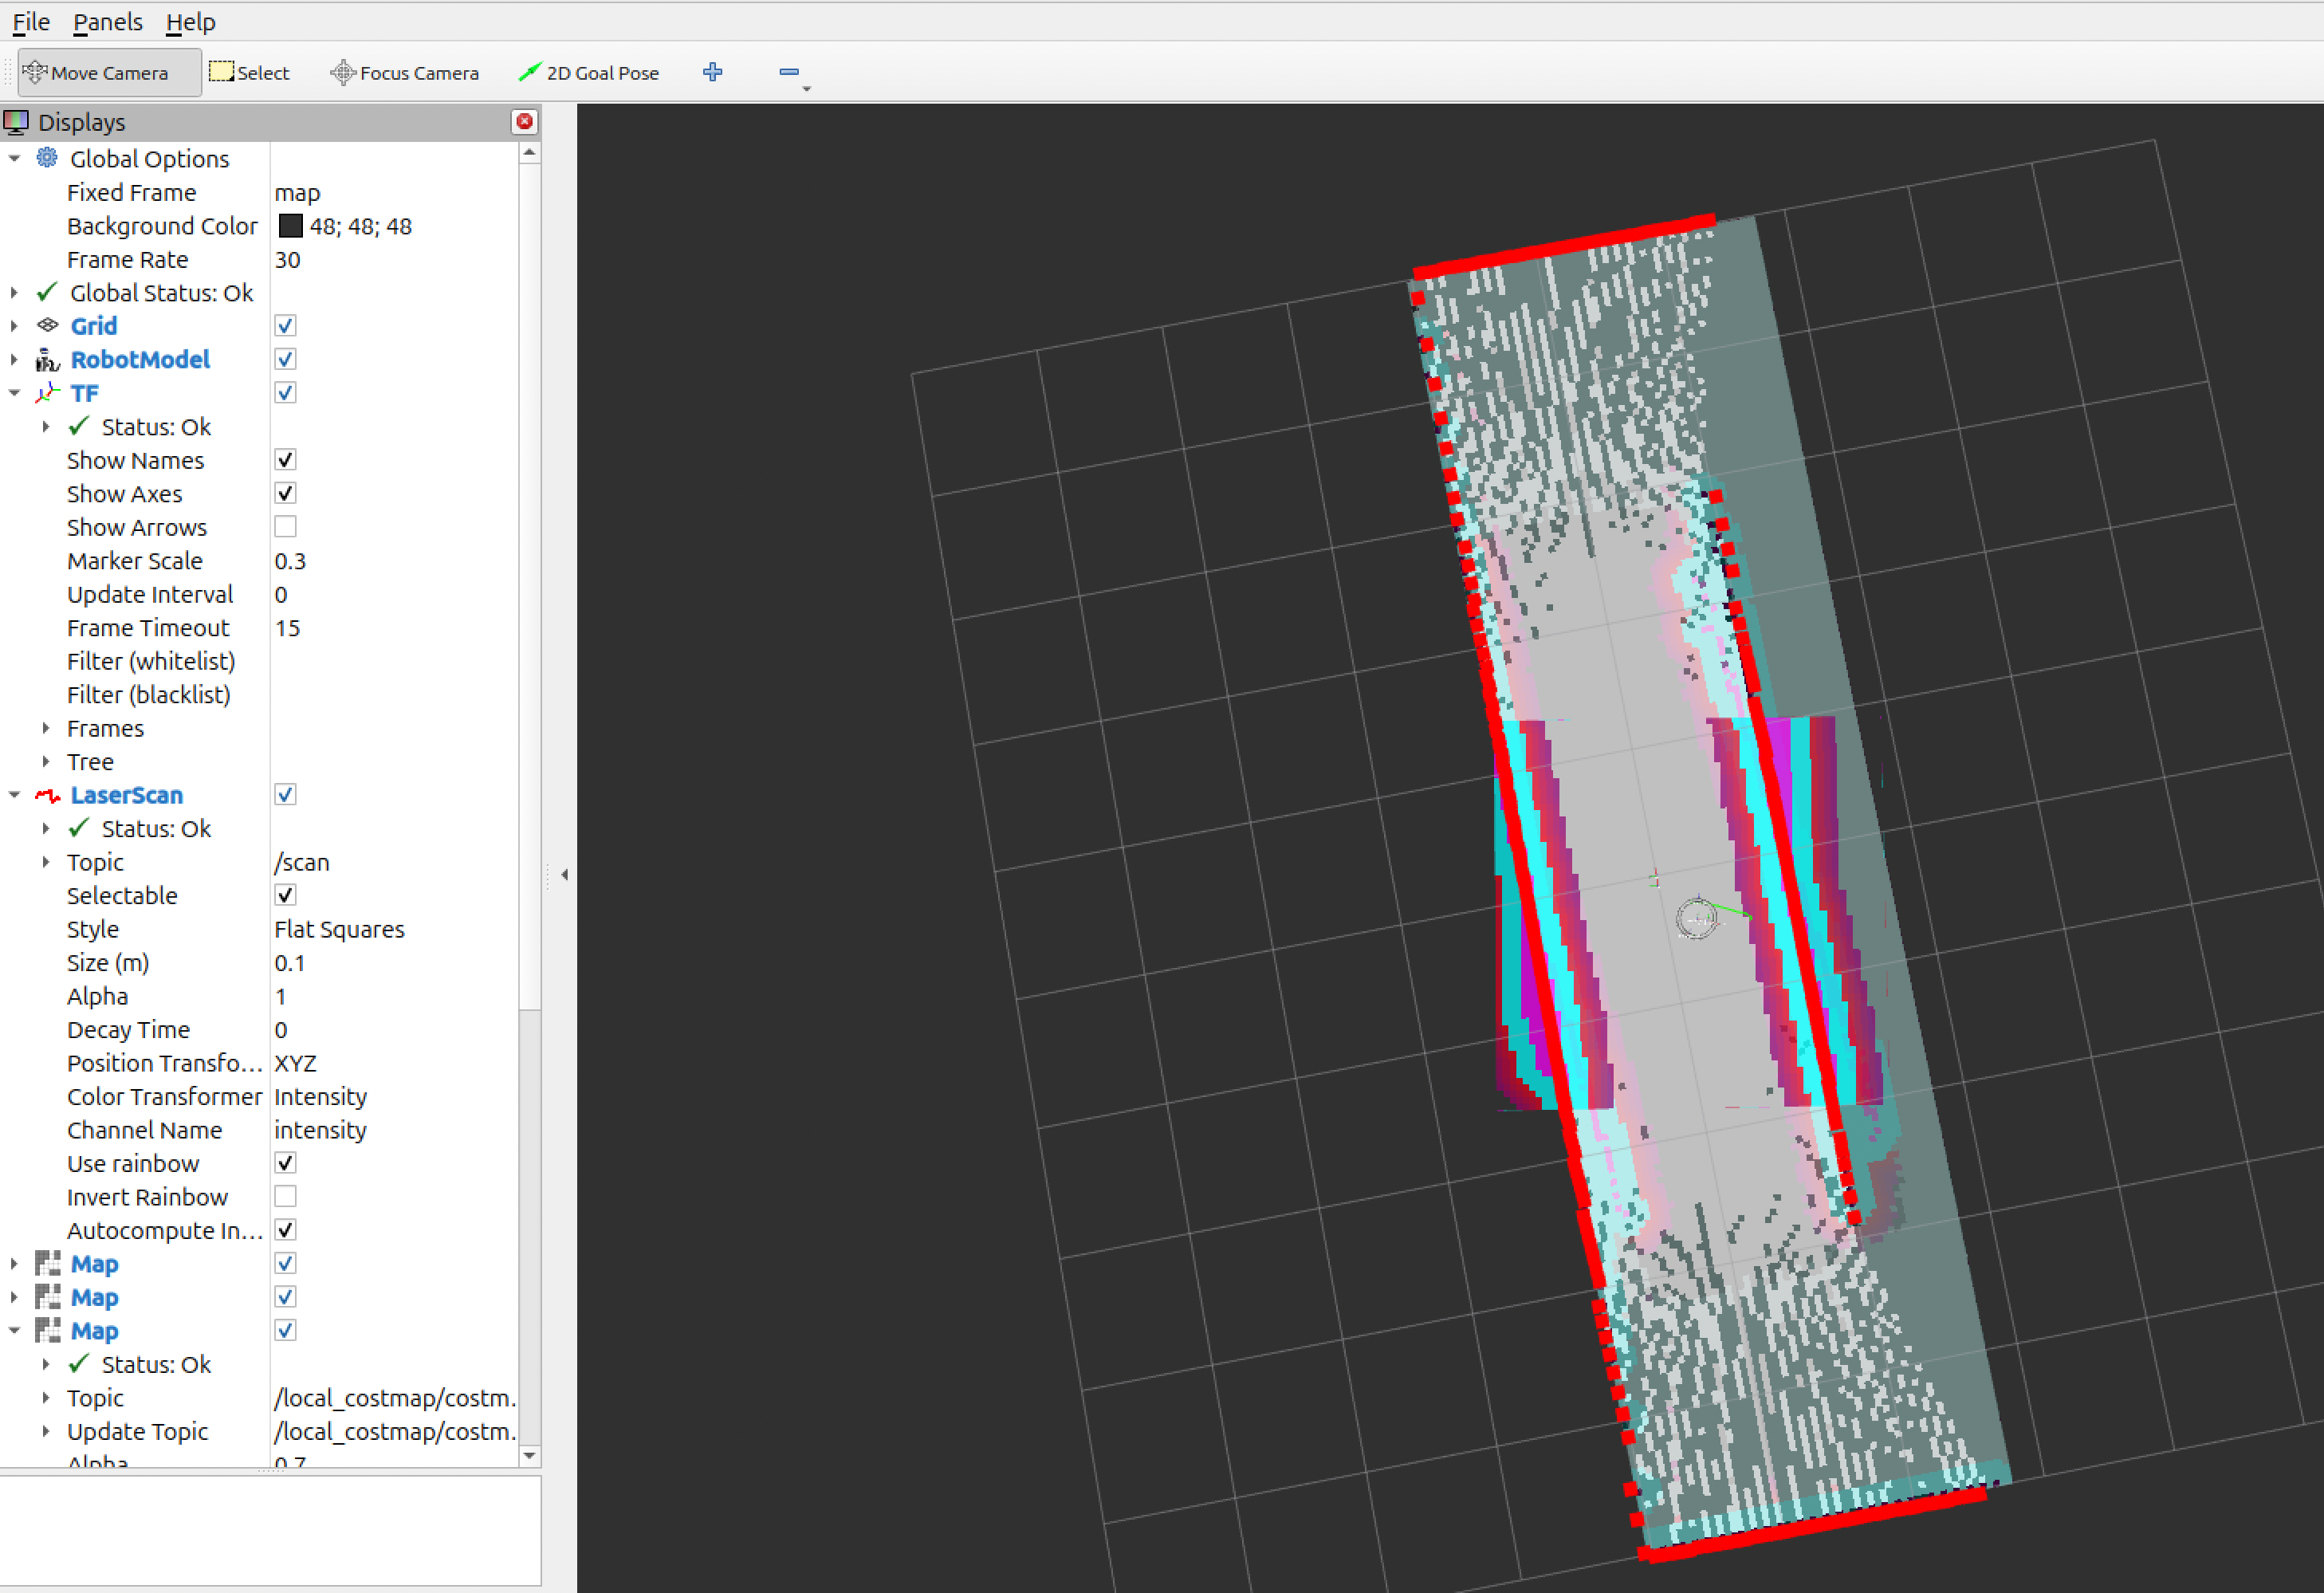
\includegraphics[width=\columnwidth]{fig/09_image.png}
        \caption{Start. Only the first corridor is mapped.}
    \end{subfigure}
    \begin{subfigure}{\columnwidth}
        \centering
        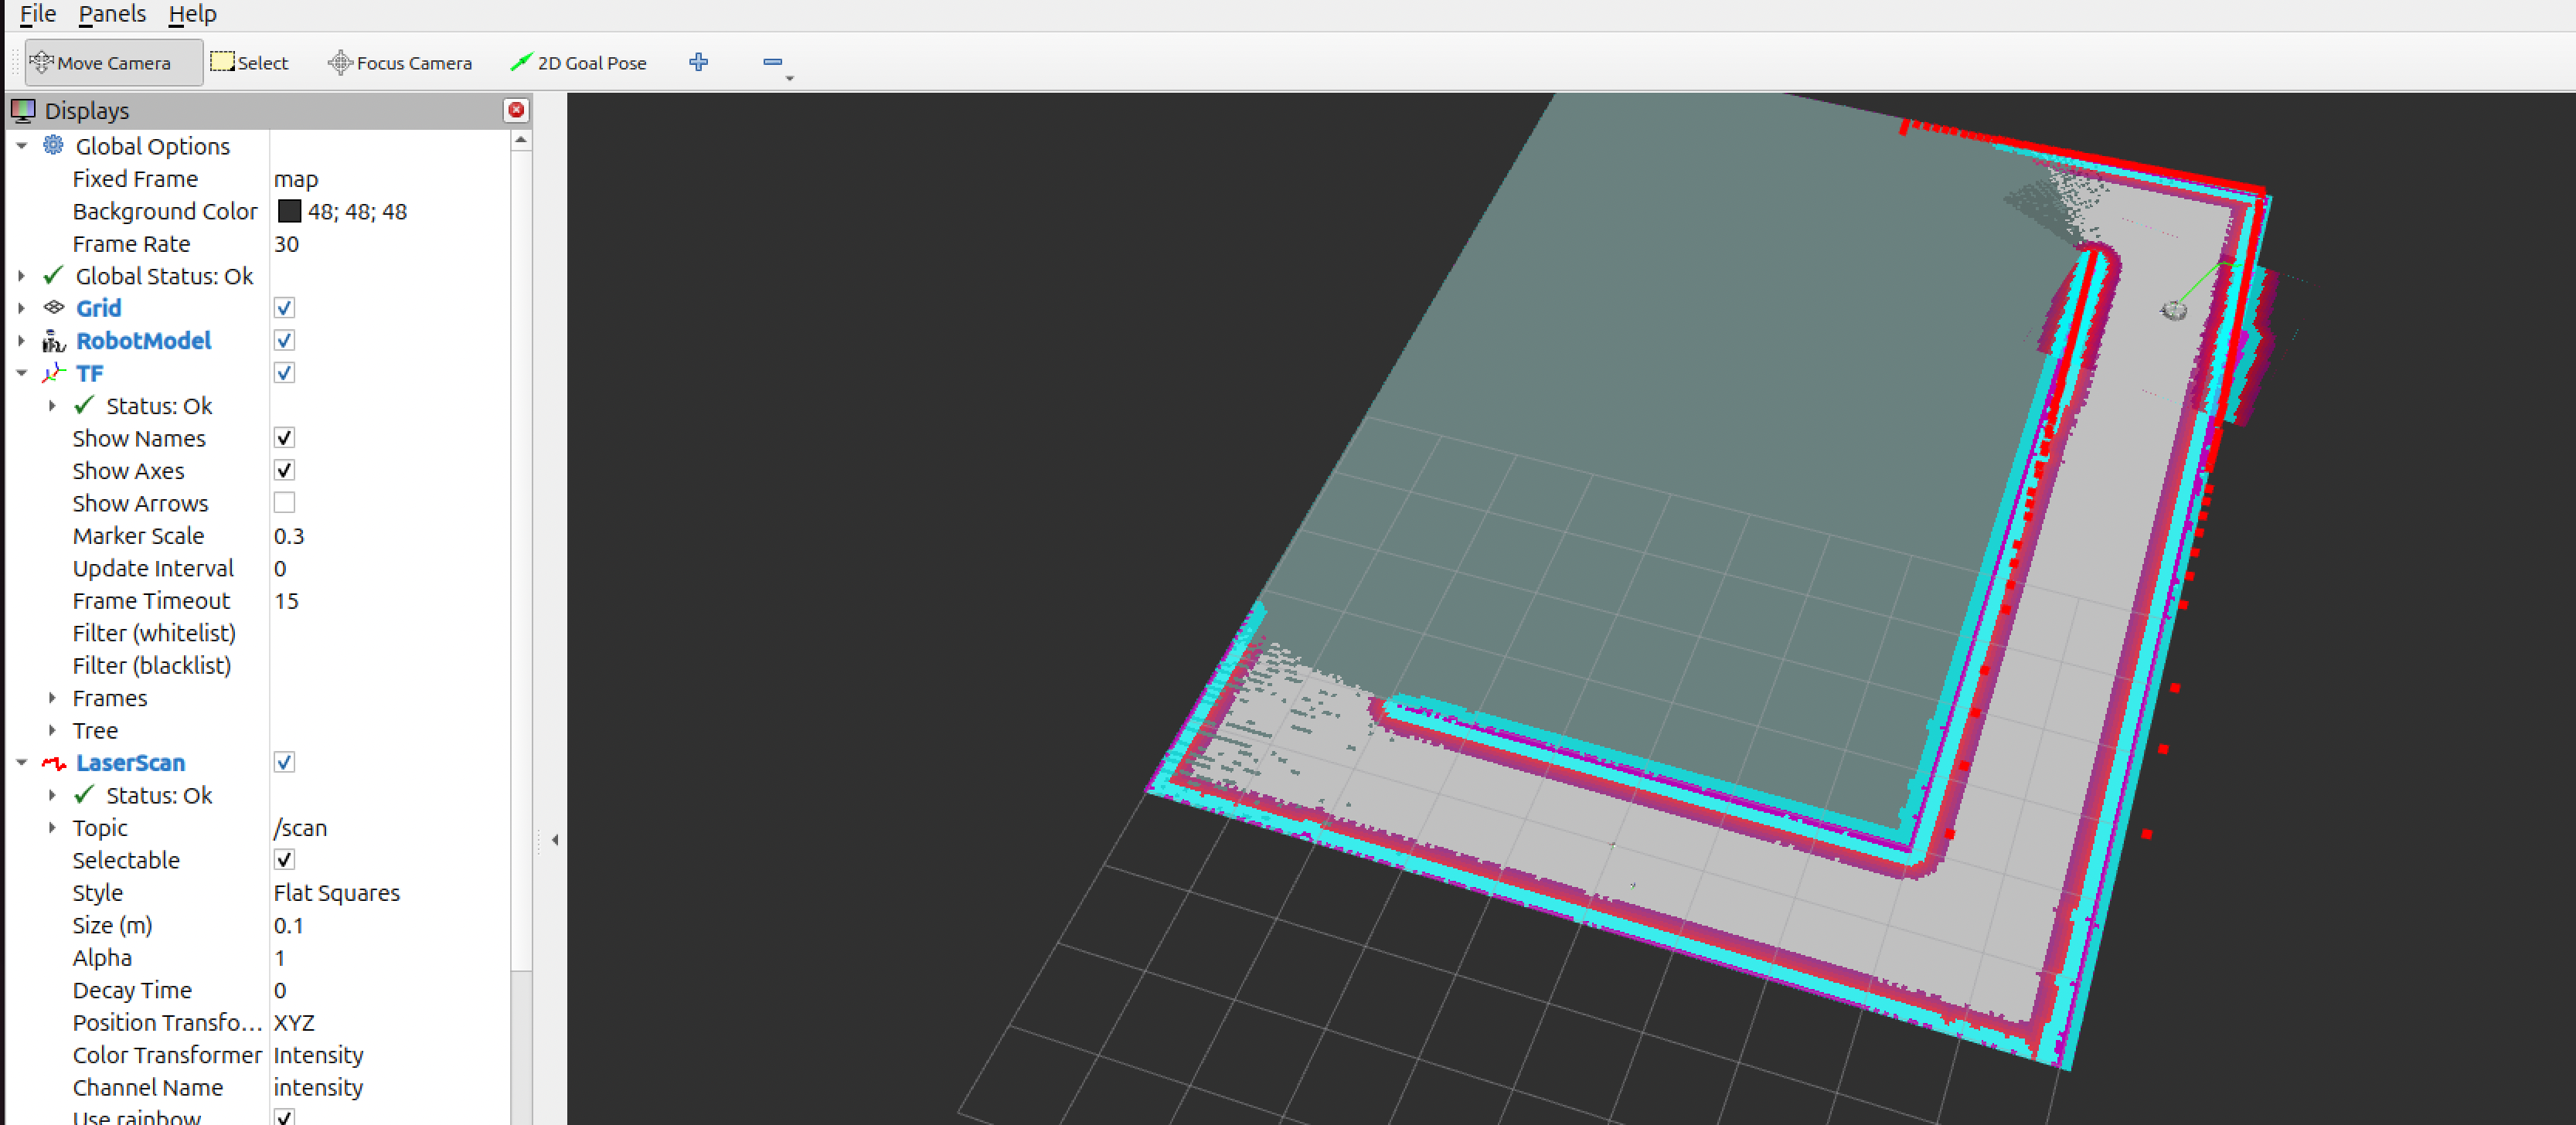
\includegraphics[width=\columnwidth]{fig/10_image.png}
        \caption{The robot has followed the corridor around the first corner.}
    \end{subfigure}
    \caption{The first part of the exploration.}
    \label{fig:explore1}
\end{figure}

\begin{figure}[H]
    \centering
    \begin{subfigure}{\columnwidth}
        \centering
        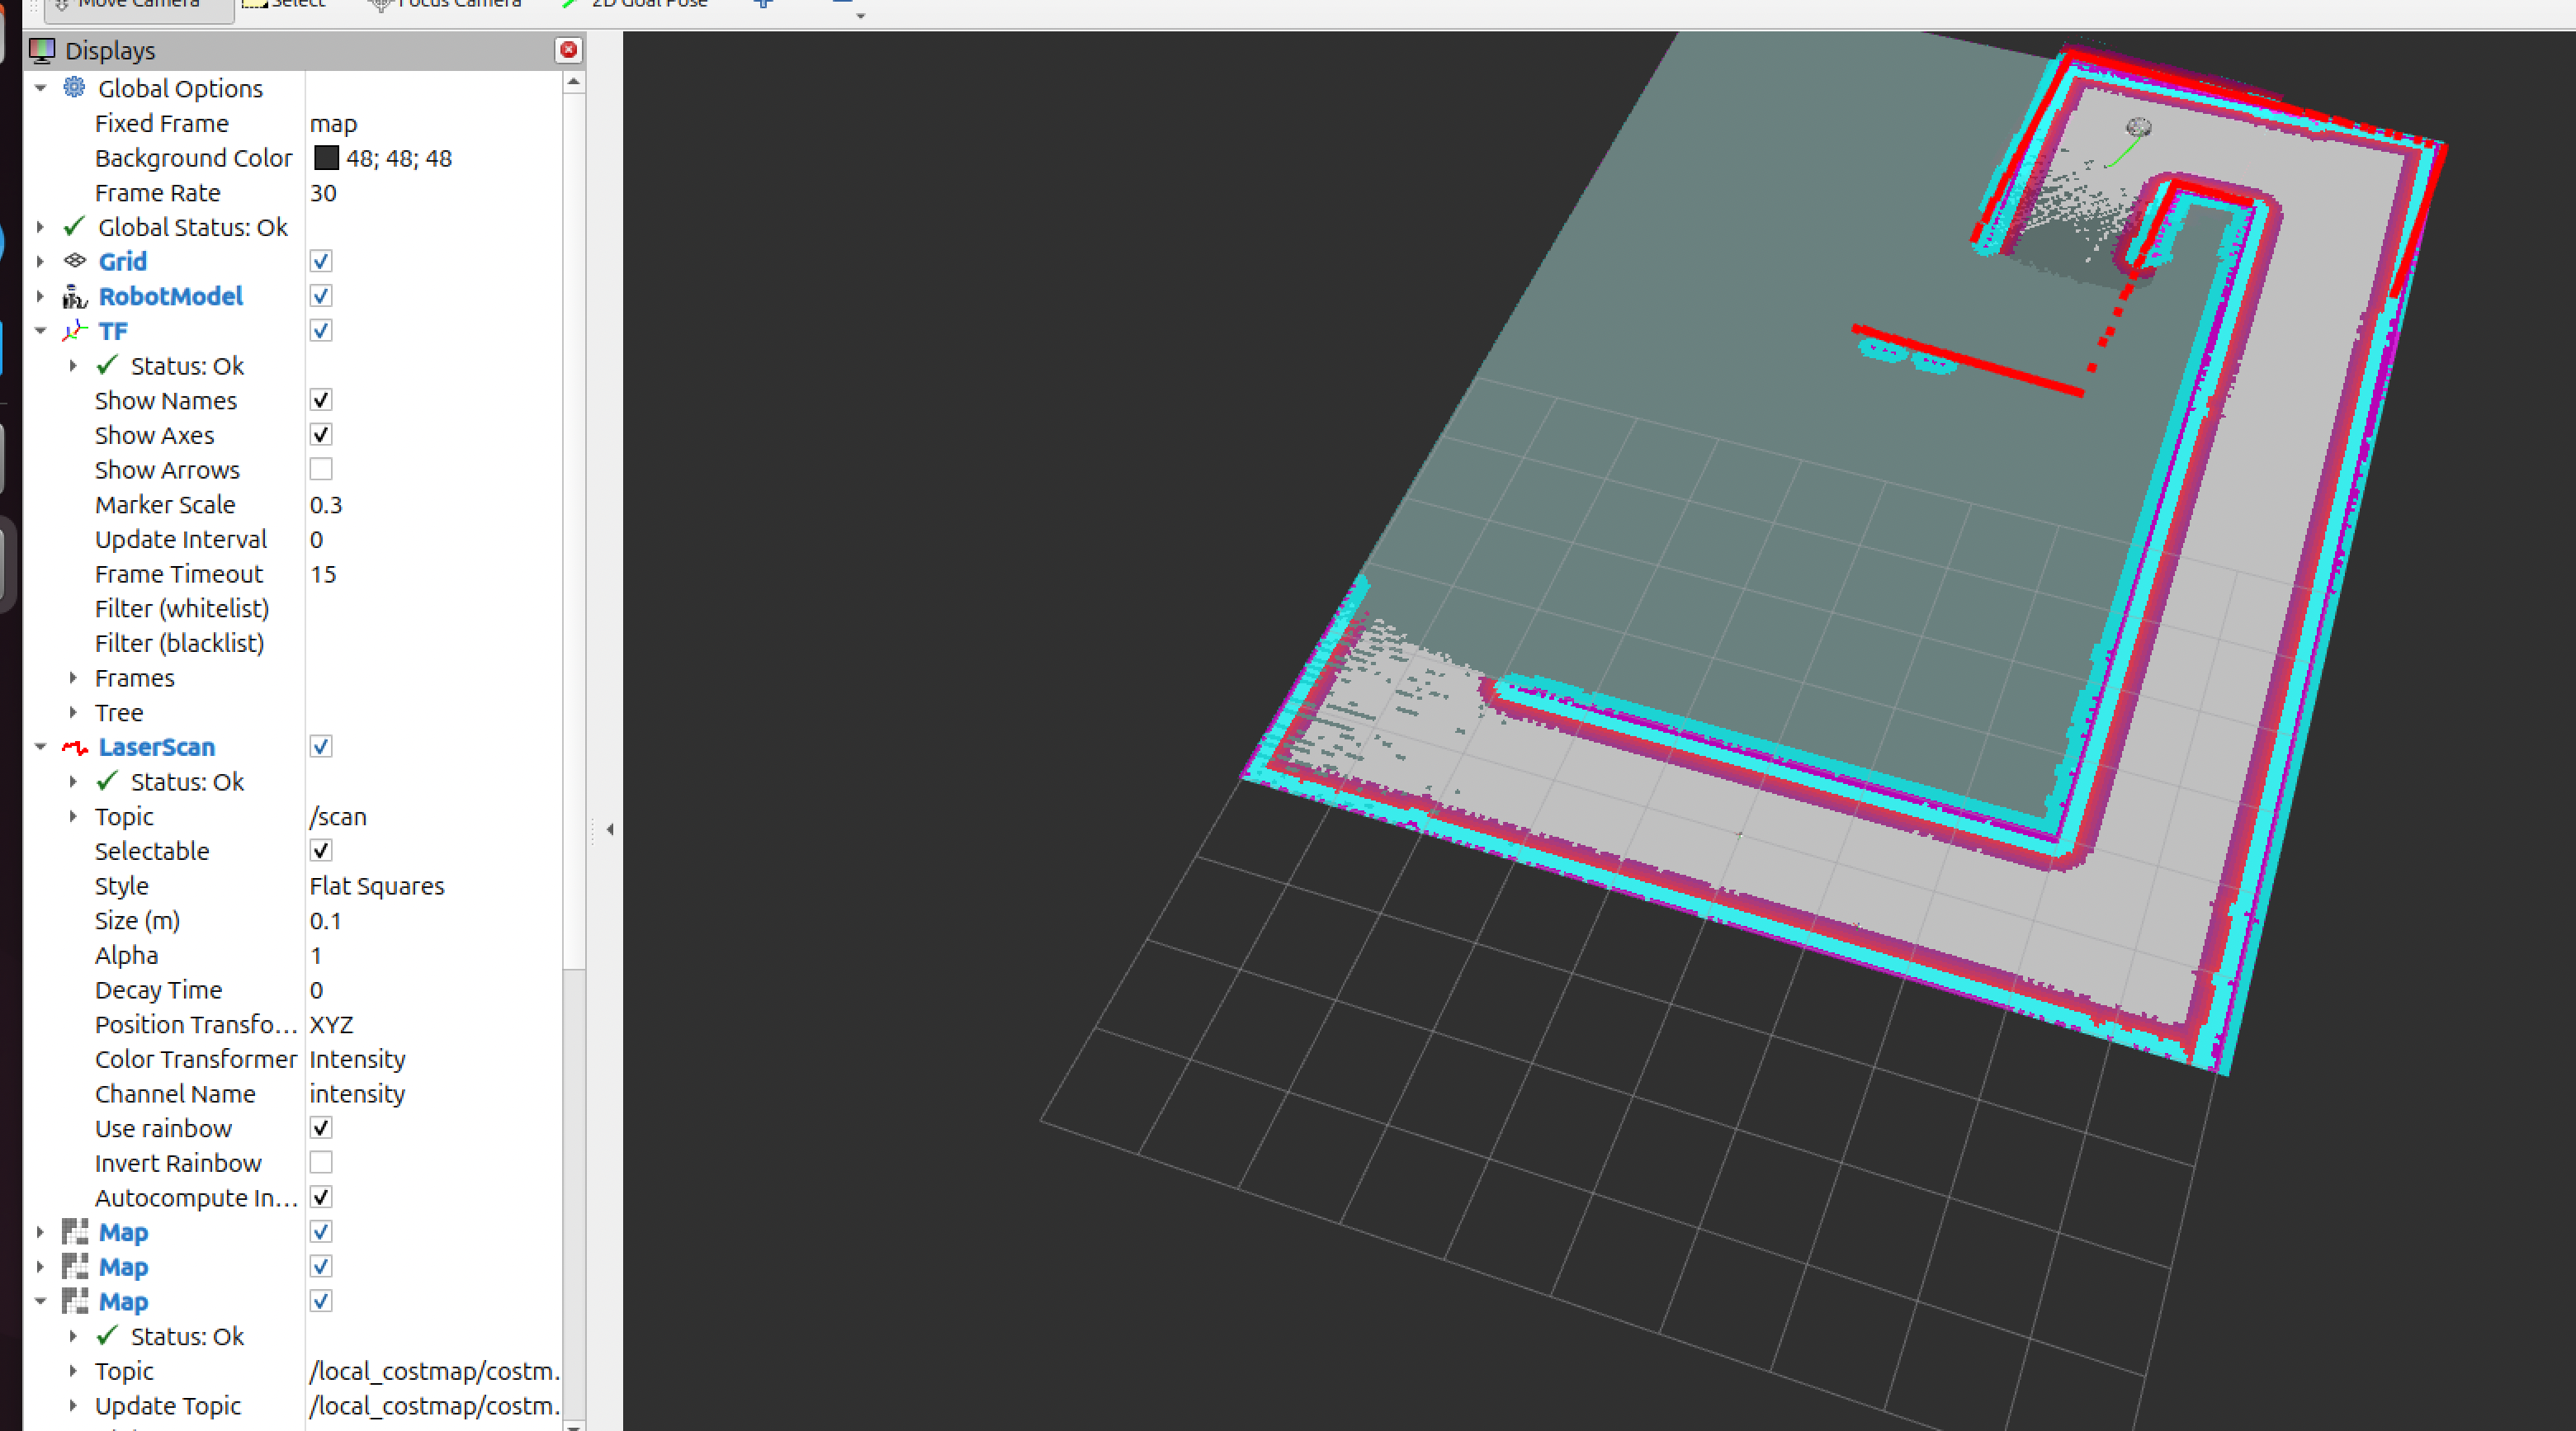
\includegraphics[width=\columnwidth]{fig/11_image.png}
        \caption{The robot is mapping the top of the maze.}
    \end{subfigure}
    \begin{subfigure}{\columnwidth}
        \centering
        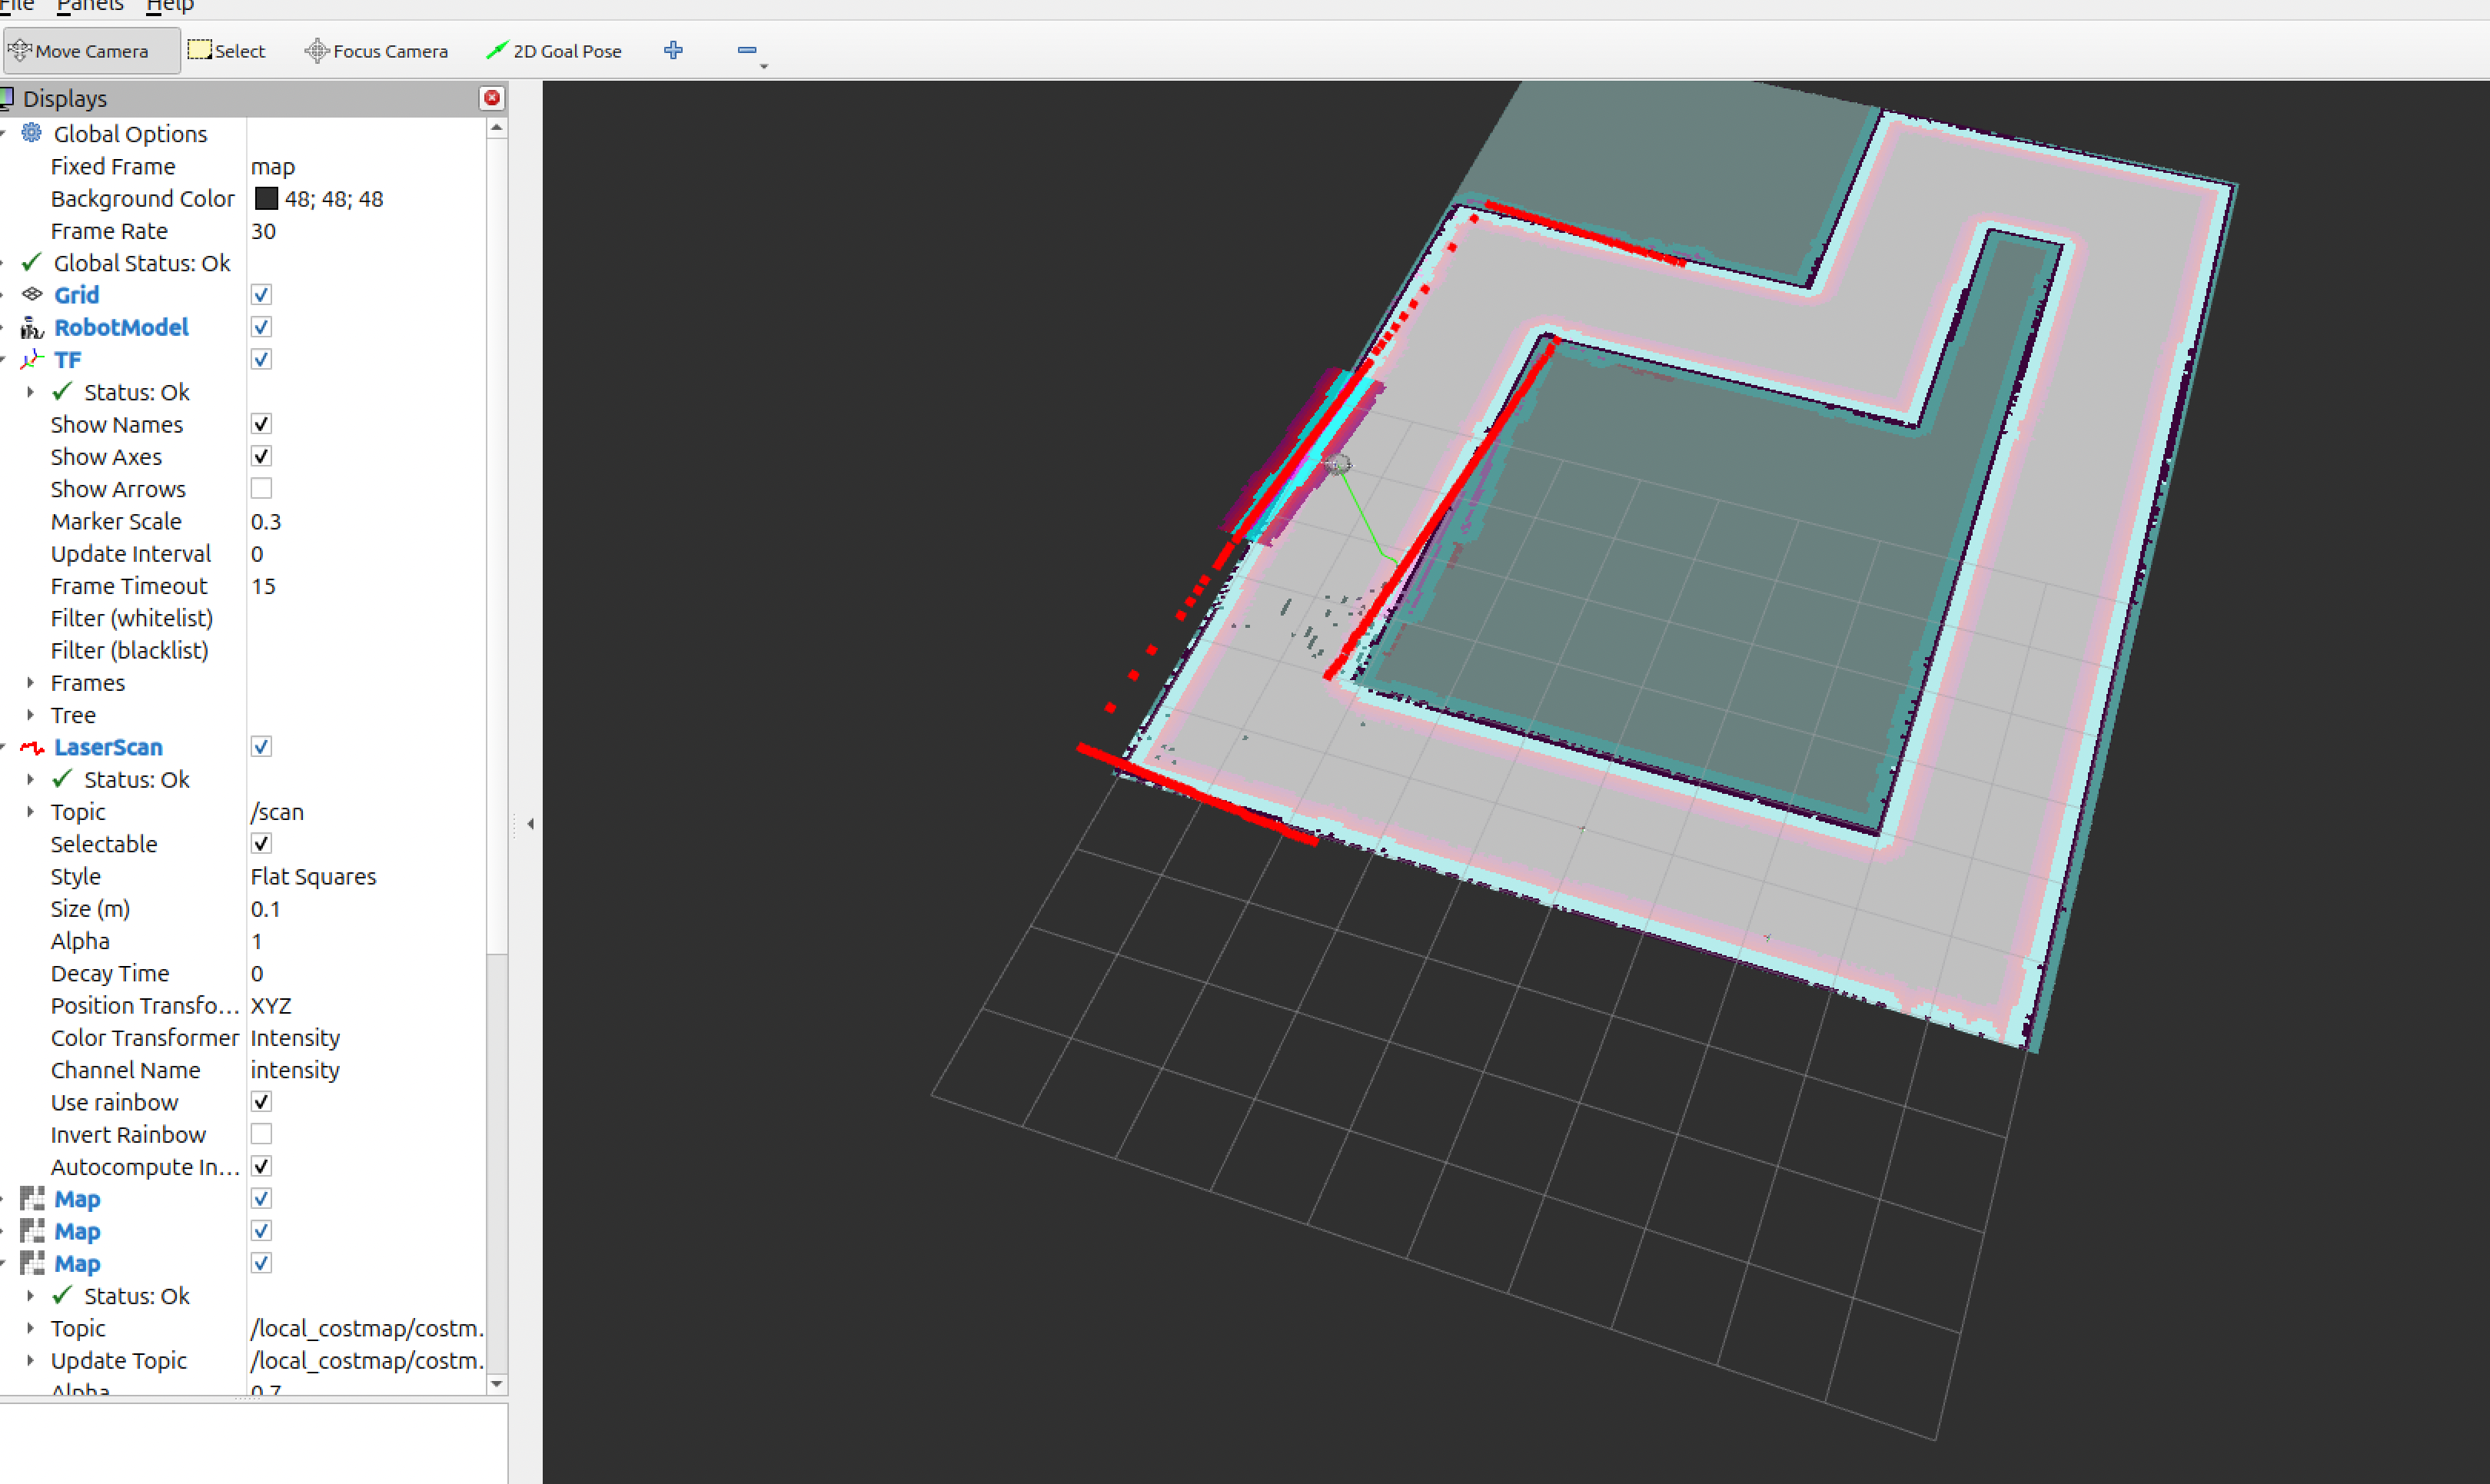
\includegraphics[width=\columnwidth]{fig/12_image.png}
        \caption{End. The whole maze is mapped, but the scan on the left does
                 not line up with the map.}
    \end{subfigure}
    \caption{The last part of the exploration.}
    \label{fig:explore2}
\end{figure}

\section{Reflection}
This was a good assignment to implement, as we learned how costmaps can be used for exploring the maze, and it was good to see it visually. Other than this, the assignment gave us a good indication of what we wanted to do for our exam project.

\end{document}
\documentclass[conference]{IEEEtran}

\usepackage{amsmath,amssymb,amsfonts}
\usepackage{graphicx}
\usepackage{textcomp}
\usepackage{xcolor}
\usepackage{url}
\usepackage[hidelinks]{hyperref}
\usepackage{booktabs}
\usepackage{float}
\usepackage{listings}
\usepackage{subcaption}
\usepackage[newfloat]{minted}
\usepackage{tikz}
\usetikzlibrary{arrows.meta, positioning, shapes.geometric}
\pagestyle{plain}

\setminted{
    fontsize=\scriptsize,
    breaklines=true,
    bgcolor=gray!8,
    frame=none,
    xleftmargin=6pt
}

\lstdefinestyle{code}{
    backgroundcolor=\color{gray!8},
    basicstyle=\ttfamily\scriptsize,
    keywordstyle=\color{green!45!black}\bfseries,
    commentstyle=\color{gray},
    stringstyle=\color{red!60!black},
    breaklines=true,
    breakatwhitespace=false,
    postbreak=\mbox{\textcolor{gray}{$\hookrightarrow$}\space},
    frame=none,
    numbers=none,
    showstringspaces=false,
    captionpos=b,
    columns=fullflexible,
    keepspaces=true,
    xleftmargin=8pt,
    framexleftmargin=8pt,
    aboveskip=6pt,
    belowskip=6pt
}
\lstset{style=code}

% Plain style for the file tree
\lstdefinestyle{plain}{
    backgroundcolor=\color{gray!8},
    basicstyle=\ttfamily\scriptsize,
    breaklines=true,
    frame=none,
    numbers=none,
    showstringspaces=false,
    xleftmargin=8pt,
    framexleftmargin=8pt,
    aboveskip=6pt,
    belowskip=6pt
}

\raggedbottom

% Each listing below is wrapped in word counter skip markers, so the code is
% not counted. Without them texcount reads the xacro snippets as maths.

\begin{document}

\title{ACIT4820: Assignment 4}

\author{
    \IEEEauthorblockN{Felix Boehm}
    \IEEEauthorblockA{OsloMet \\ feboe8099@oslomet.no}
     \and
    \IEEEauthorblockN{Thomas Heim}
    \IEEEauthorblockA{OsloMet \\ thhei7342@oslomet.no}
}

\maketitle

\section{Design Choices and Method}
As we talked about in class, this assignment was not mandatory to finish. We
decided to mainly show screenshots in the results of what we have done, and not write so much text.



\section{Results}

\subsection{Task 2}

Fig.~\ref{fig:costmap} shows both the global and the local costmap. The cyan
cells along the walls are where the robot would hit the wall, and the purple
and pink cells are the inflation around it. The local costmap is the
3\,$\times$\,3\,m square around the robot, where the bands are brighter.

\begin{figure}[H]
    \centering
    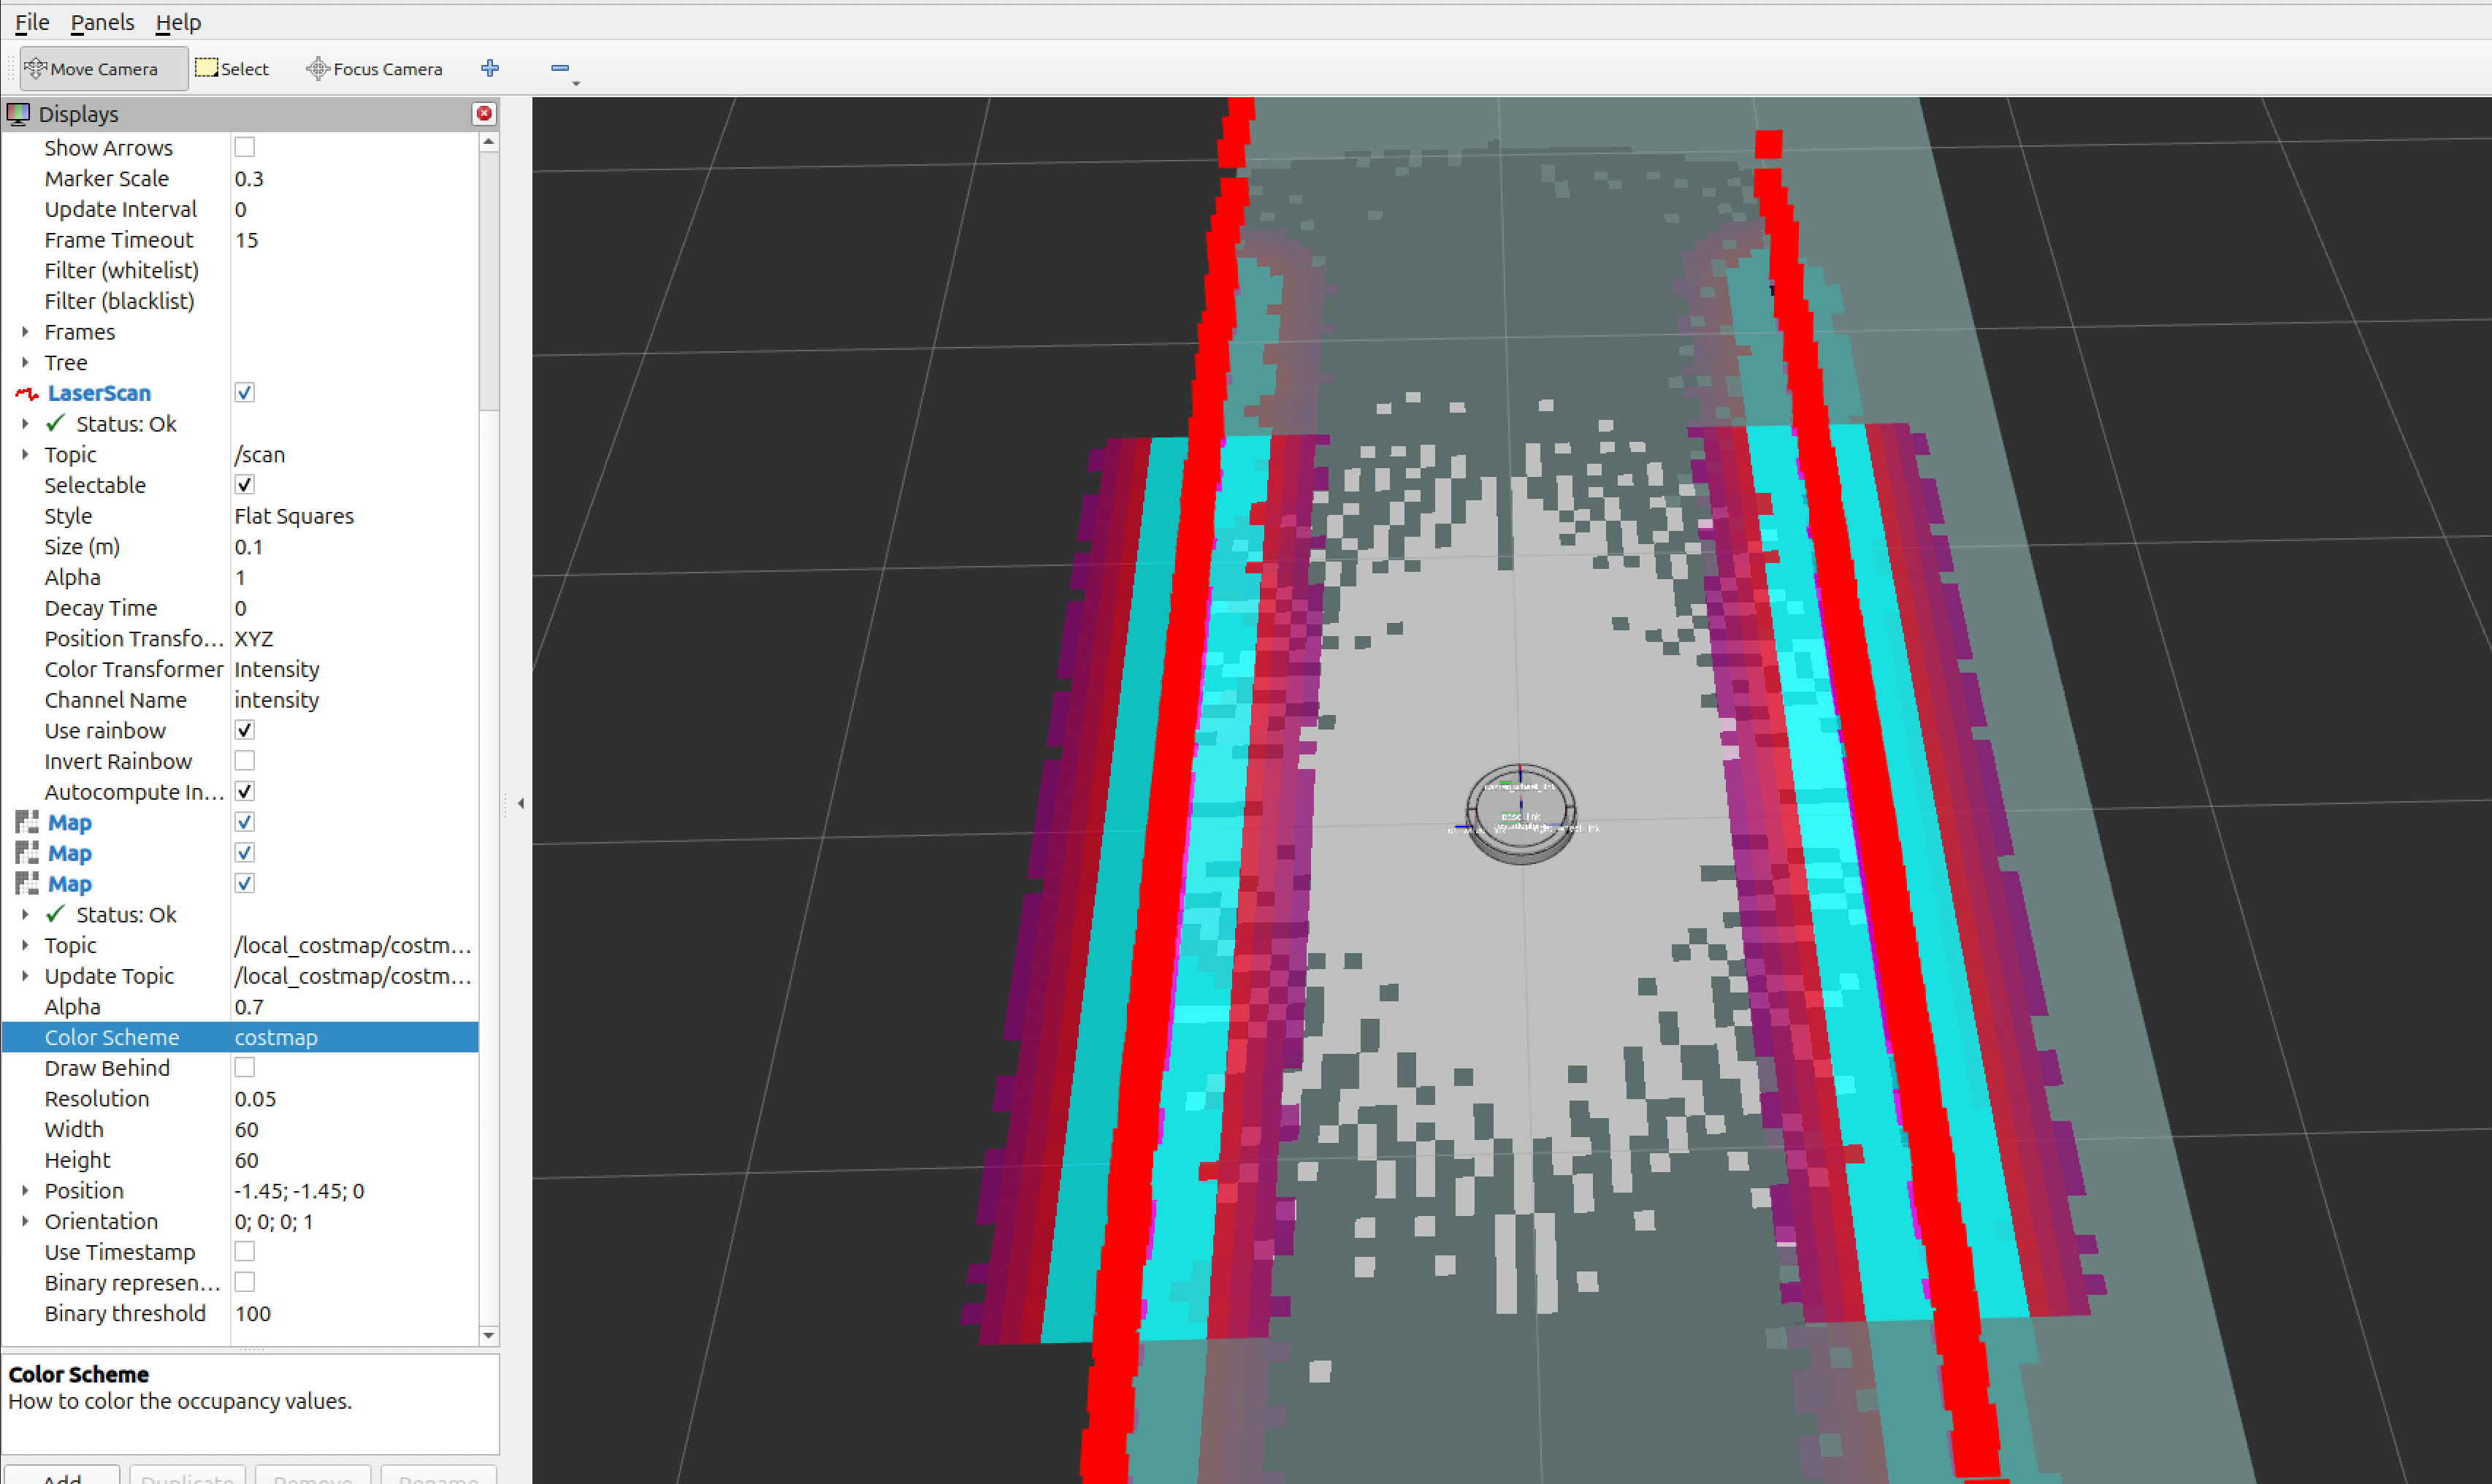
\includegraphics[width=\columnwidth]{fig/00_image.png}
    \caption{The global and local costmap around the robot. The grey path in
             the middle is free space.}
    \label{fig:costmap}
\end{figure}

We then sent the robot to goals with the 2D Goal Pose tool in RViz, as we can
see in Fig.~\ref{fig:goal1} to Fig.~\ref{fig:goal4}. The green line is the
path Nav2 planned to the goal. The map grows as the robot drives, since
\texttt{slam\_toolbox} keeps mapping while Nav2 drives.

\begin{figure}[H]
    \centering
    \begin{subfigure}{\columnwidth}
        \centering
        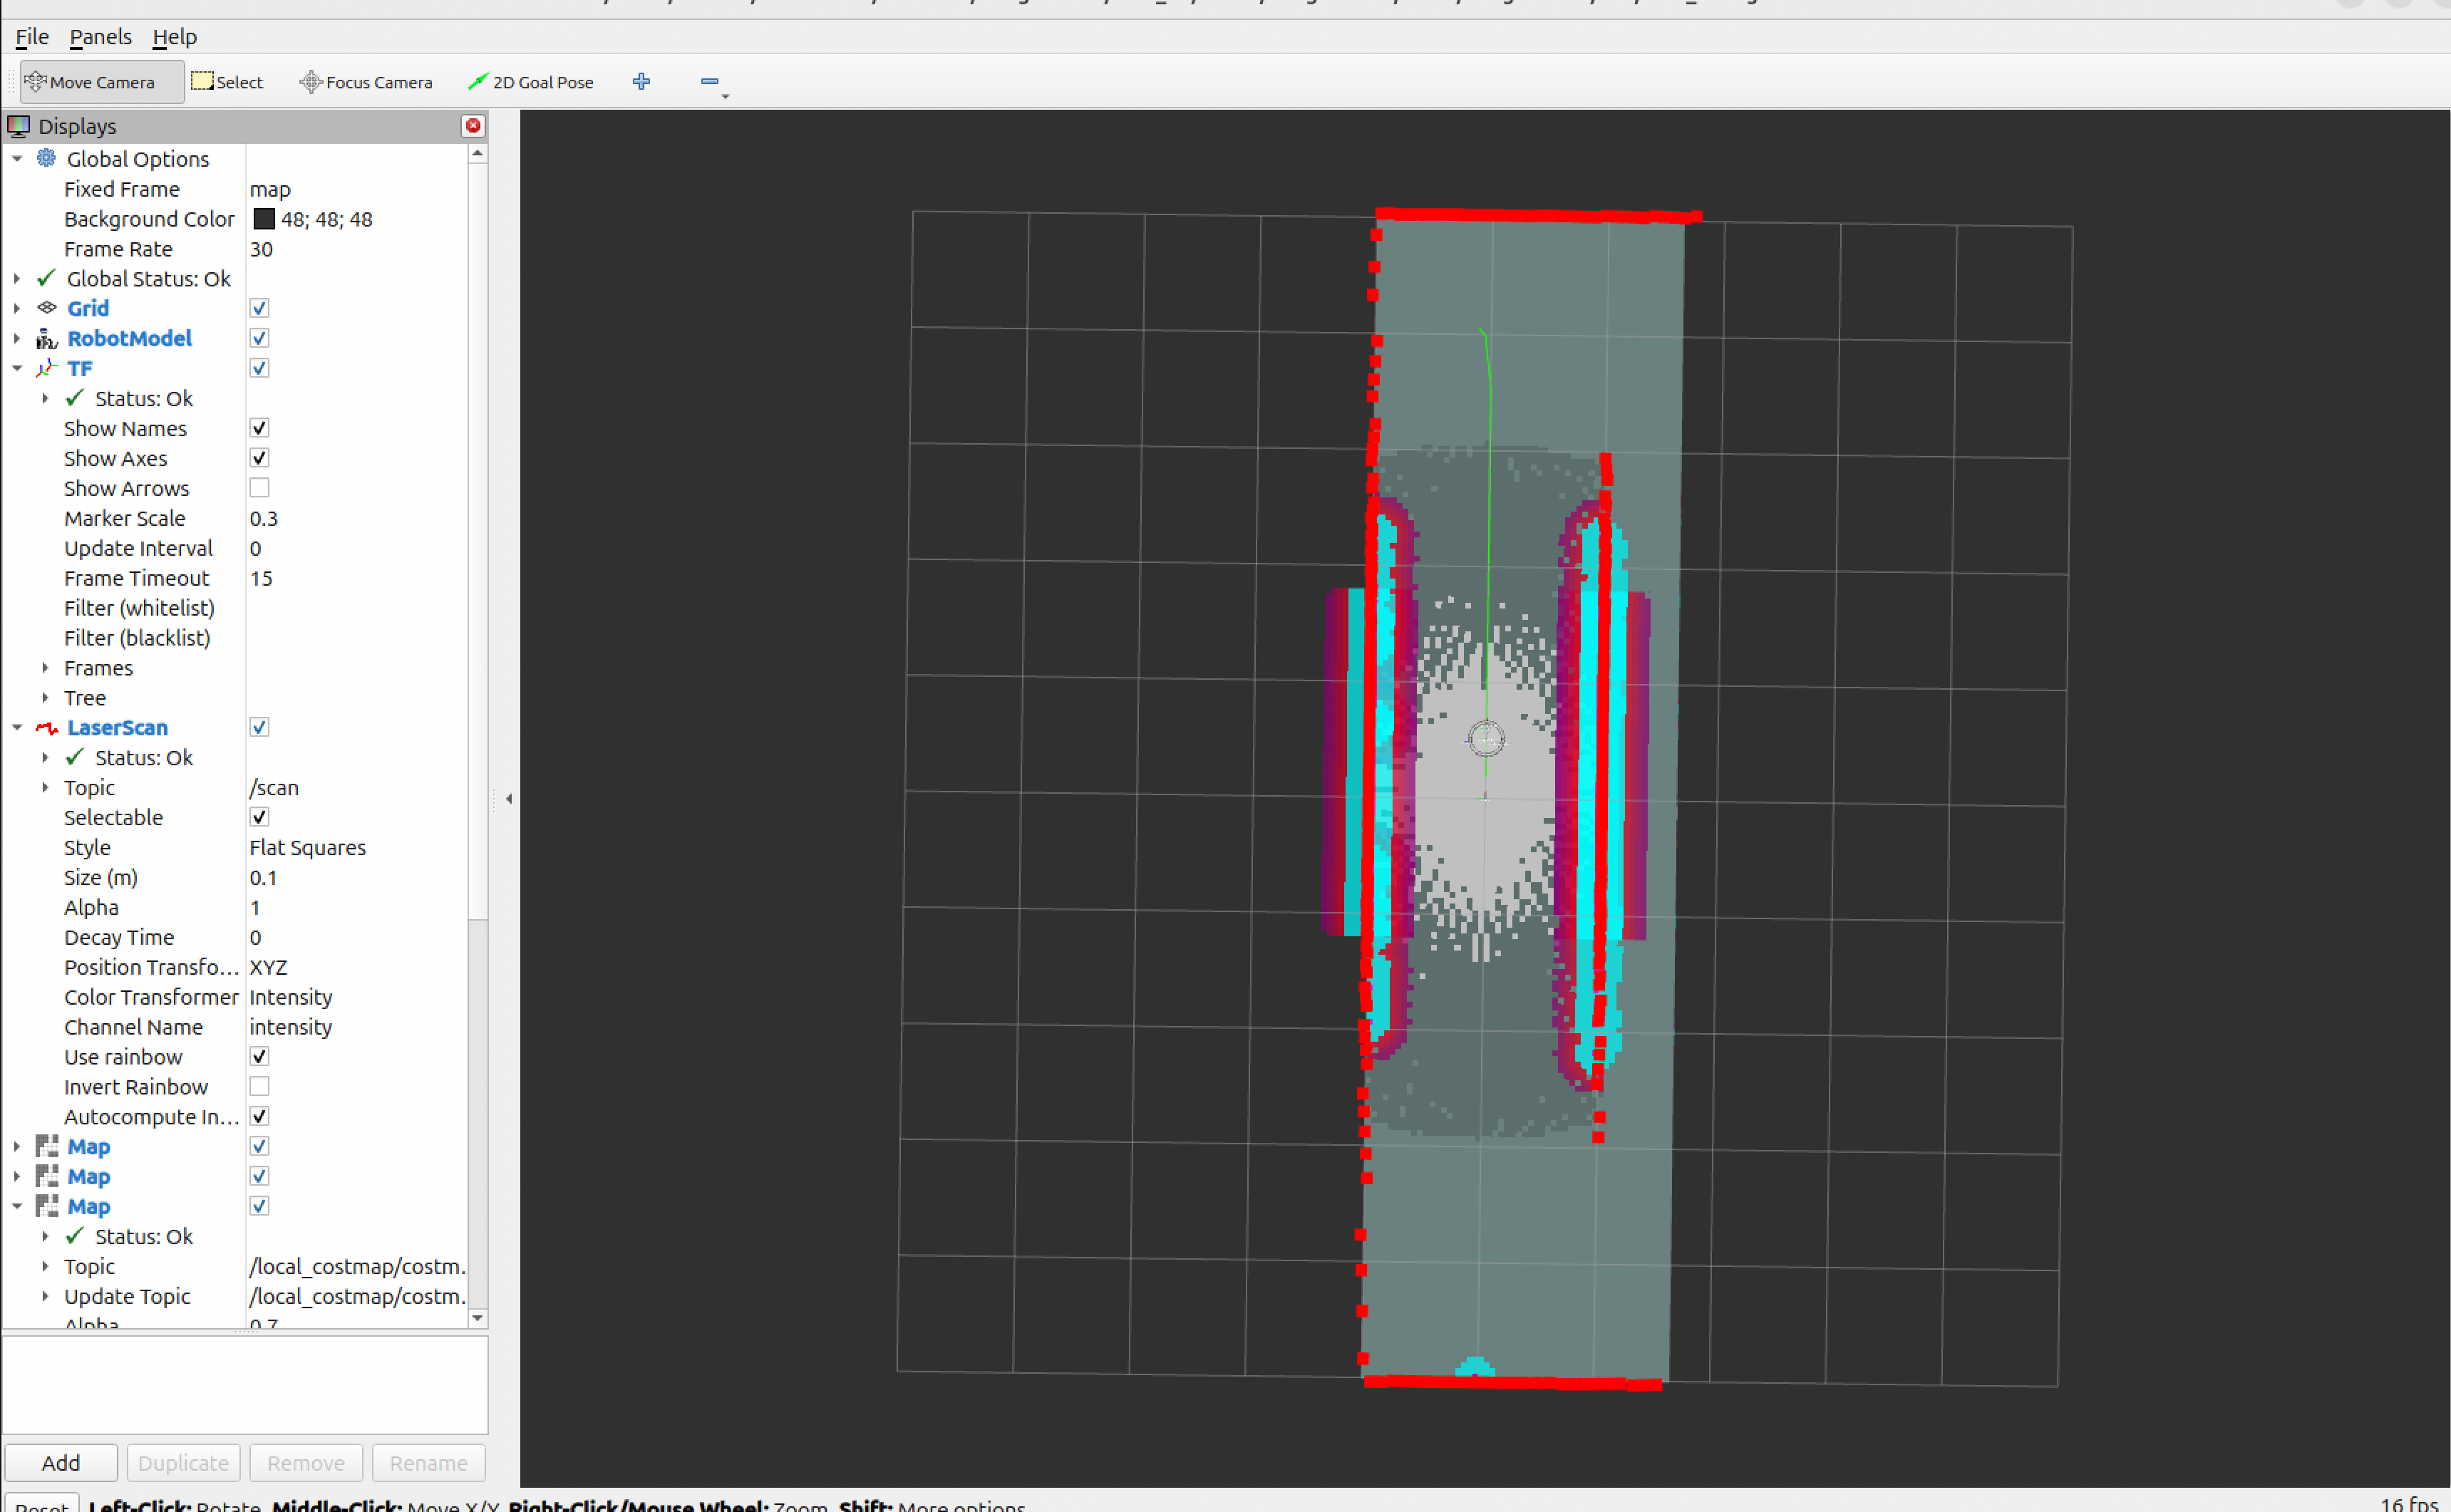
\includegraphics[width=\columnwidth]{fig/01_start.png}
        \caption{Start. The path goes straight up the corridor.}
    \end{subfigure}
    \begin{subfigure}{\columnwidth}
        \centering
        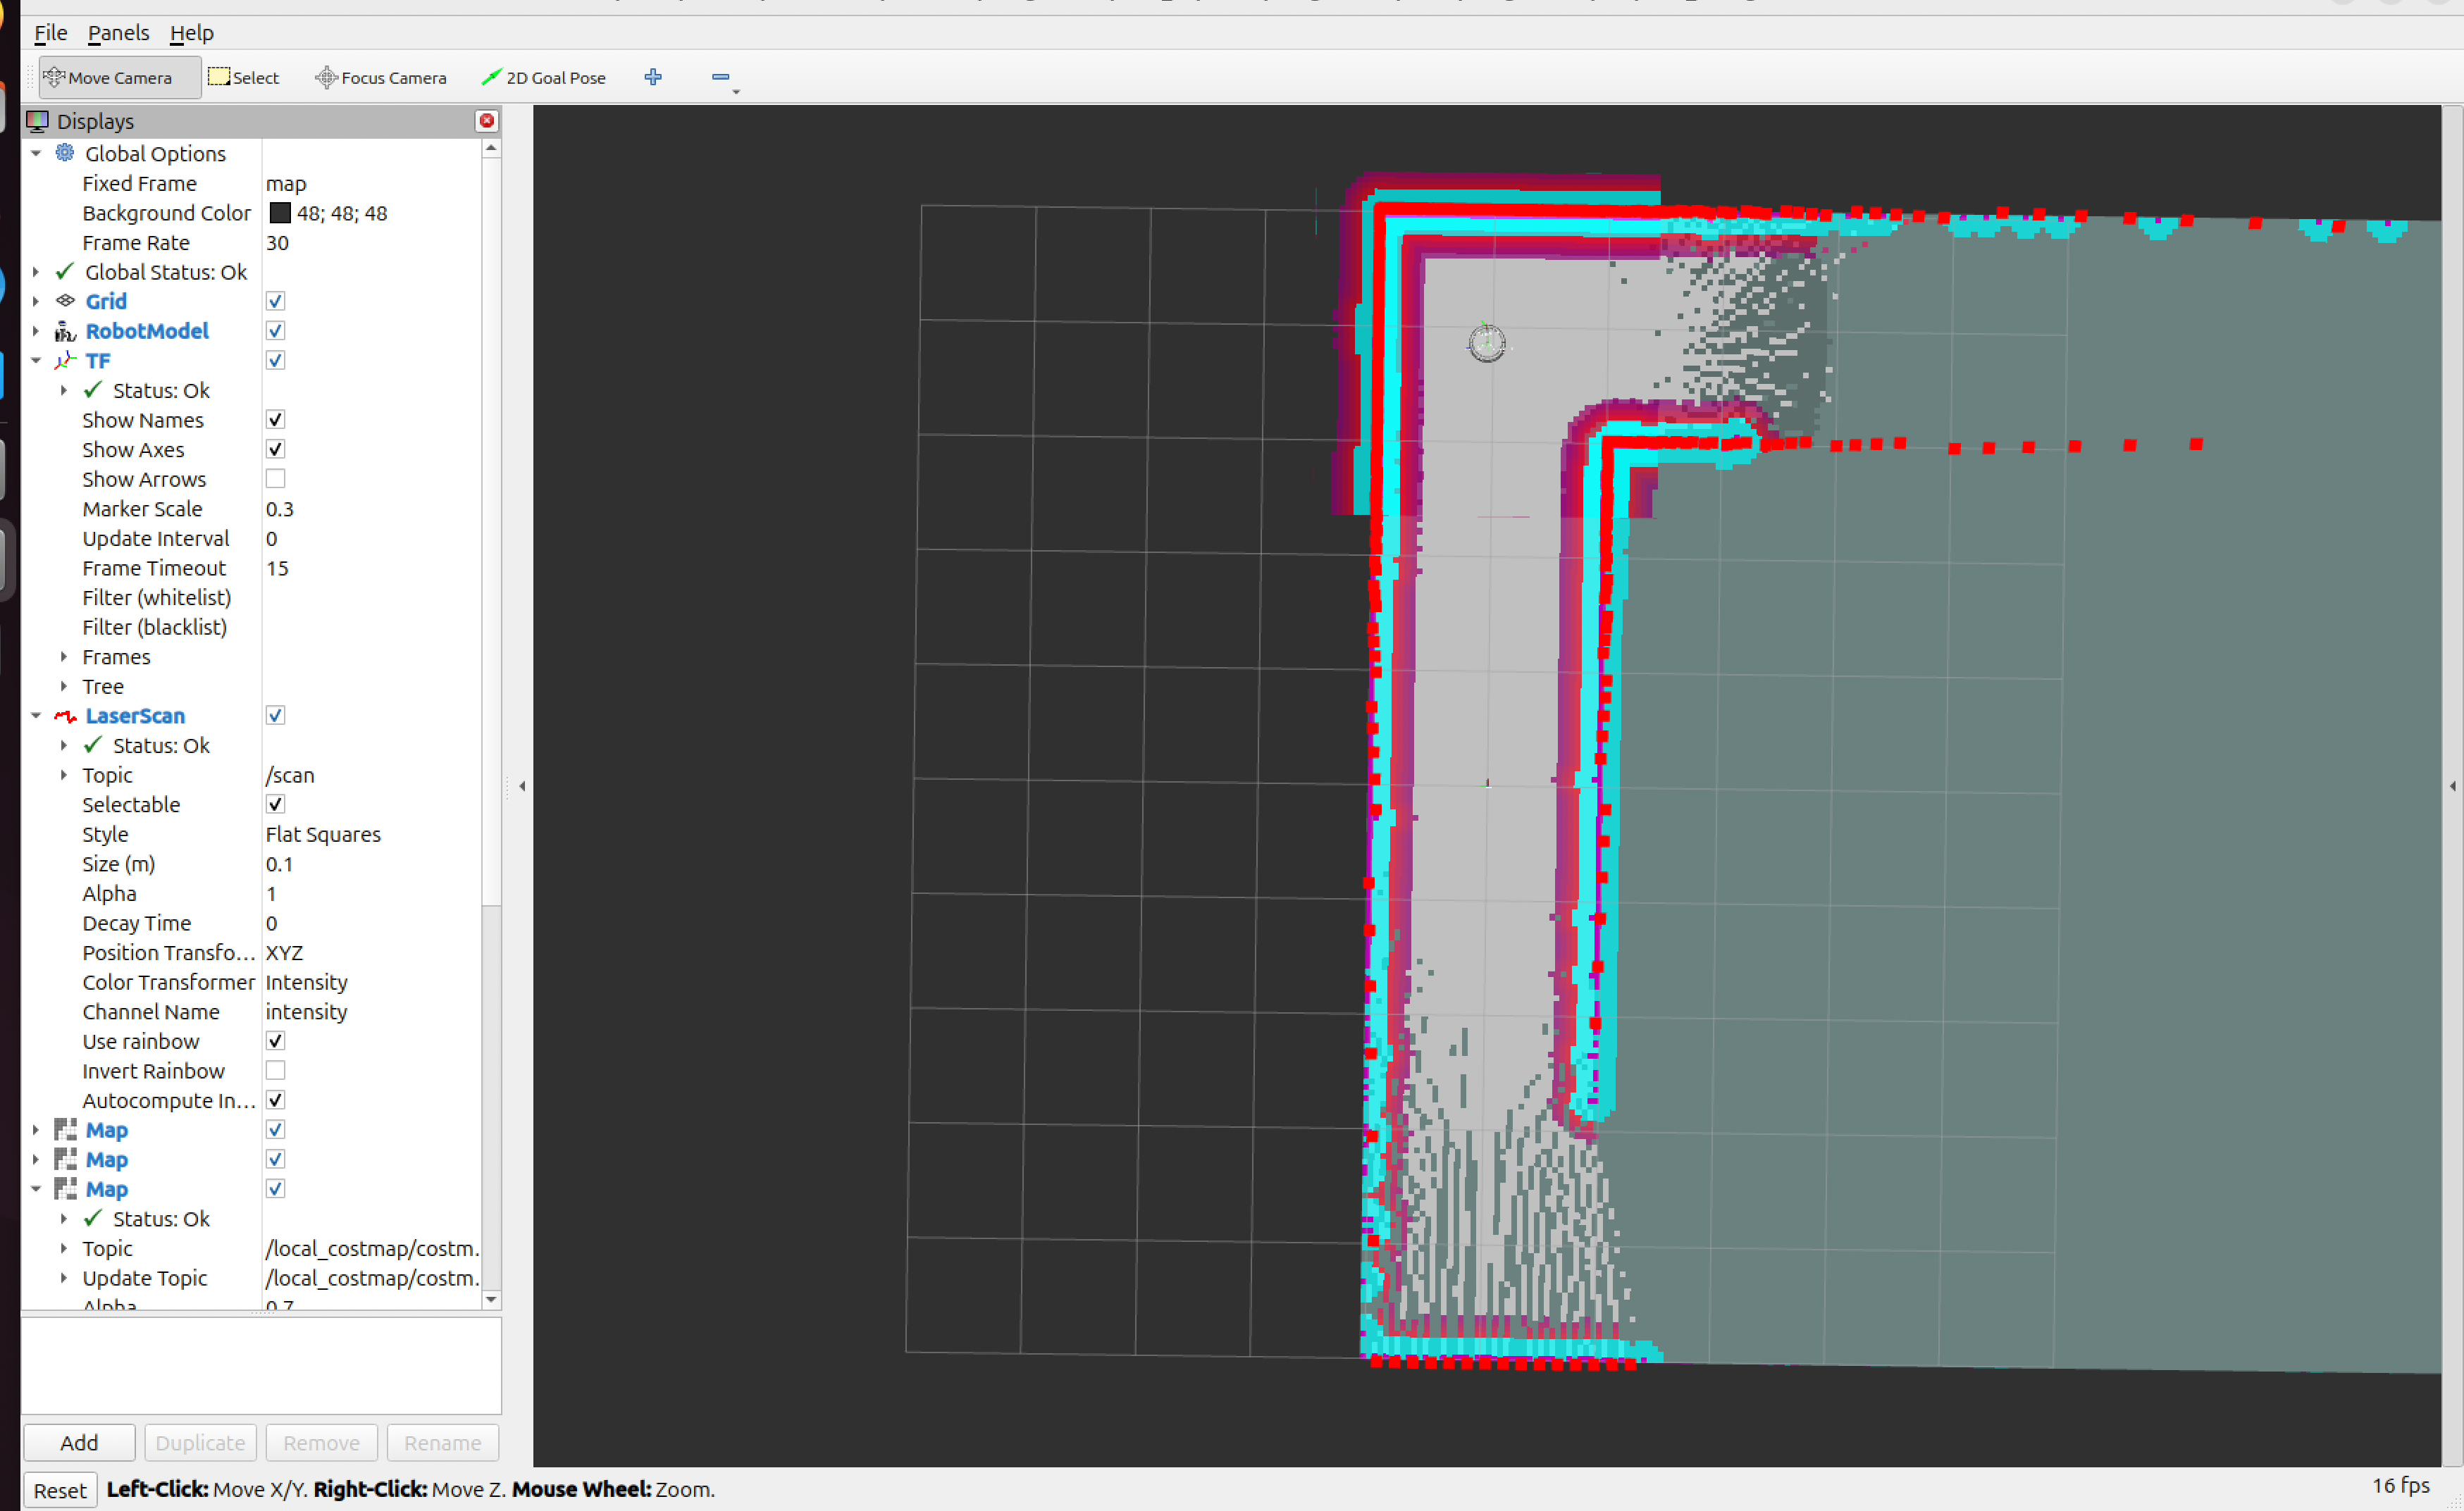
\includegraphics[width=\columnwidth]{fig/02_end.png}
        \caption{End. The robot has reached the goal and mapped the corner.}
    \end{subfigure}
    \caption{Goal 1, straight up the first corridor.}
    \label{fig:goal1}
\end{figure}

\begin{figure}[H]
    \centering
    \begin{subfigure}{\columnwidth}
        \centering
        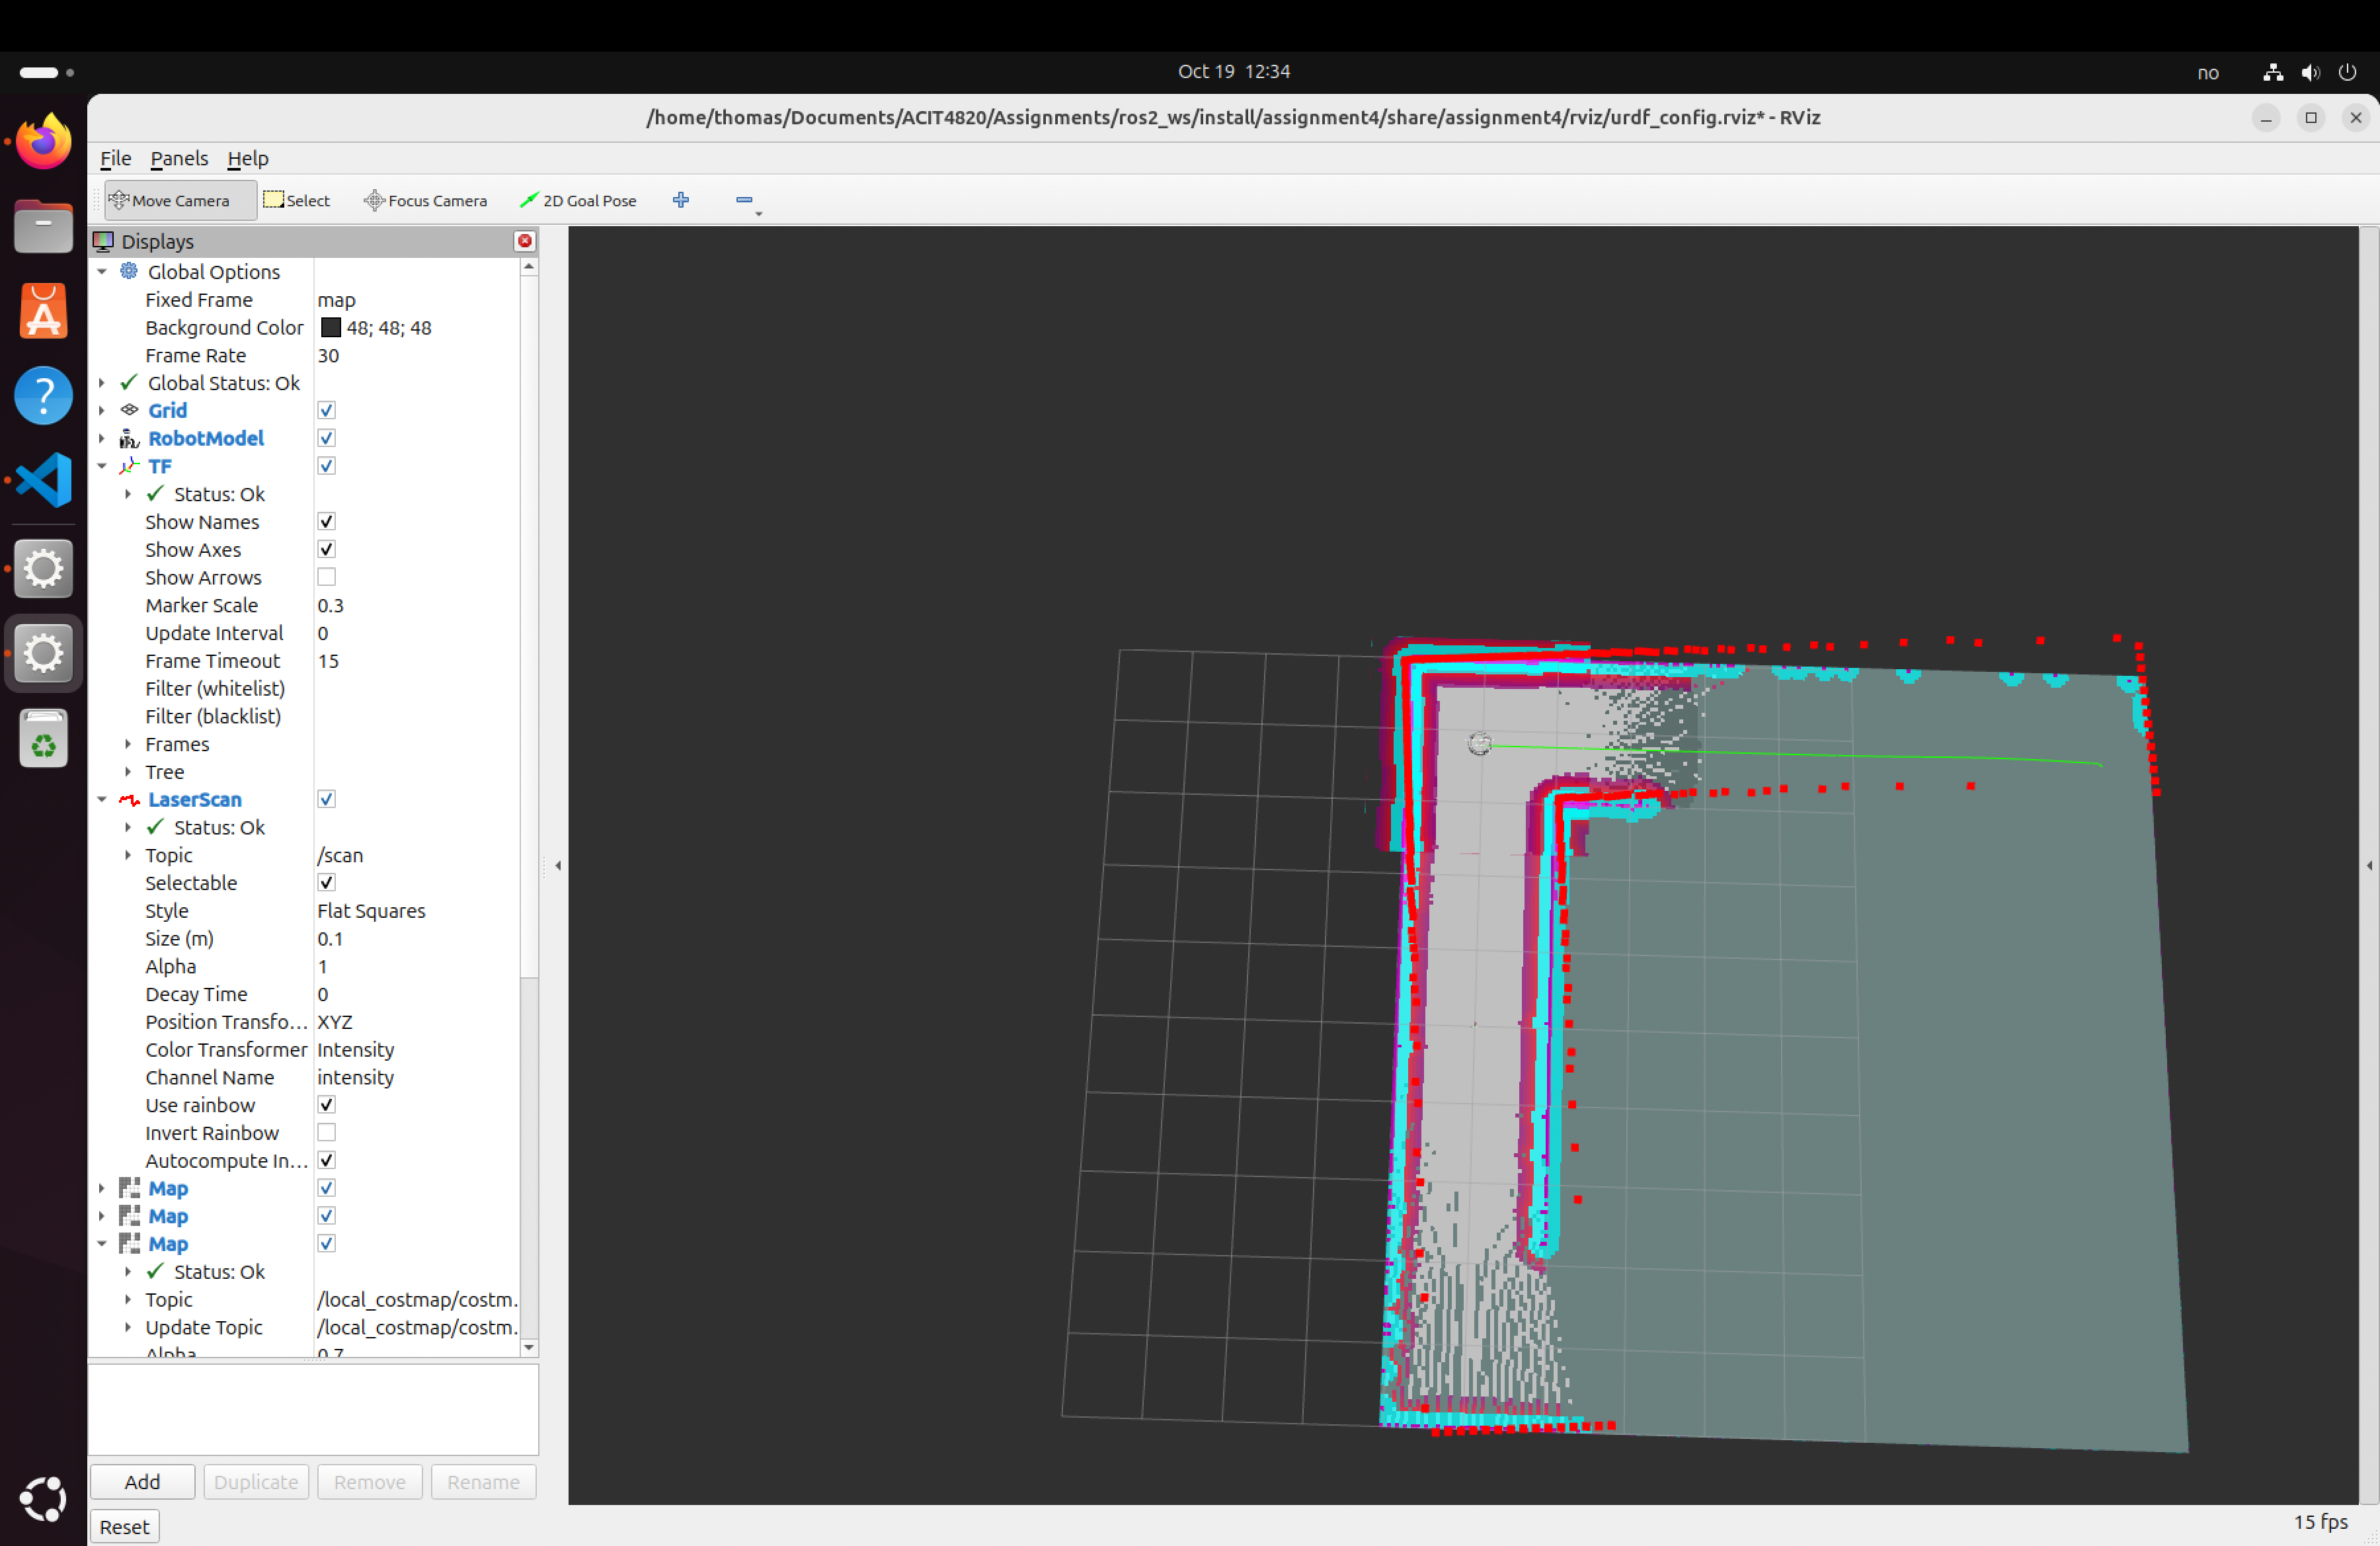
\includegraphics[width=\columnwidth]{fig/03_start.png}
        \caption{Start. The path goes around the corner.}
    \end{subfigure}
    \begin{subfigure}{\columnwidth}
        \centering
        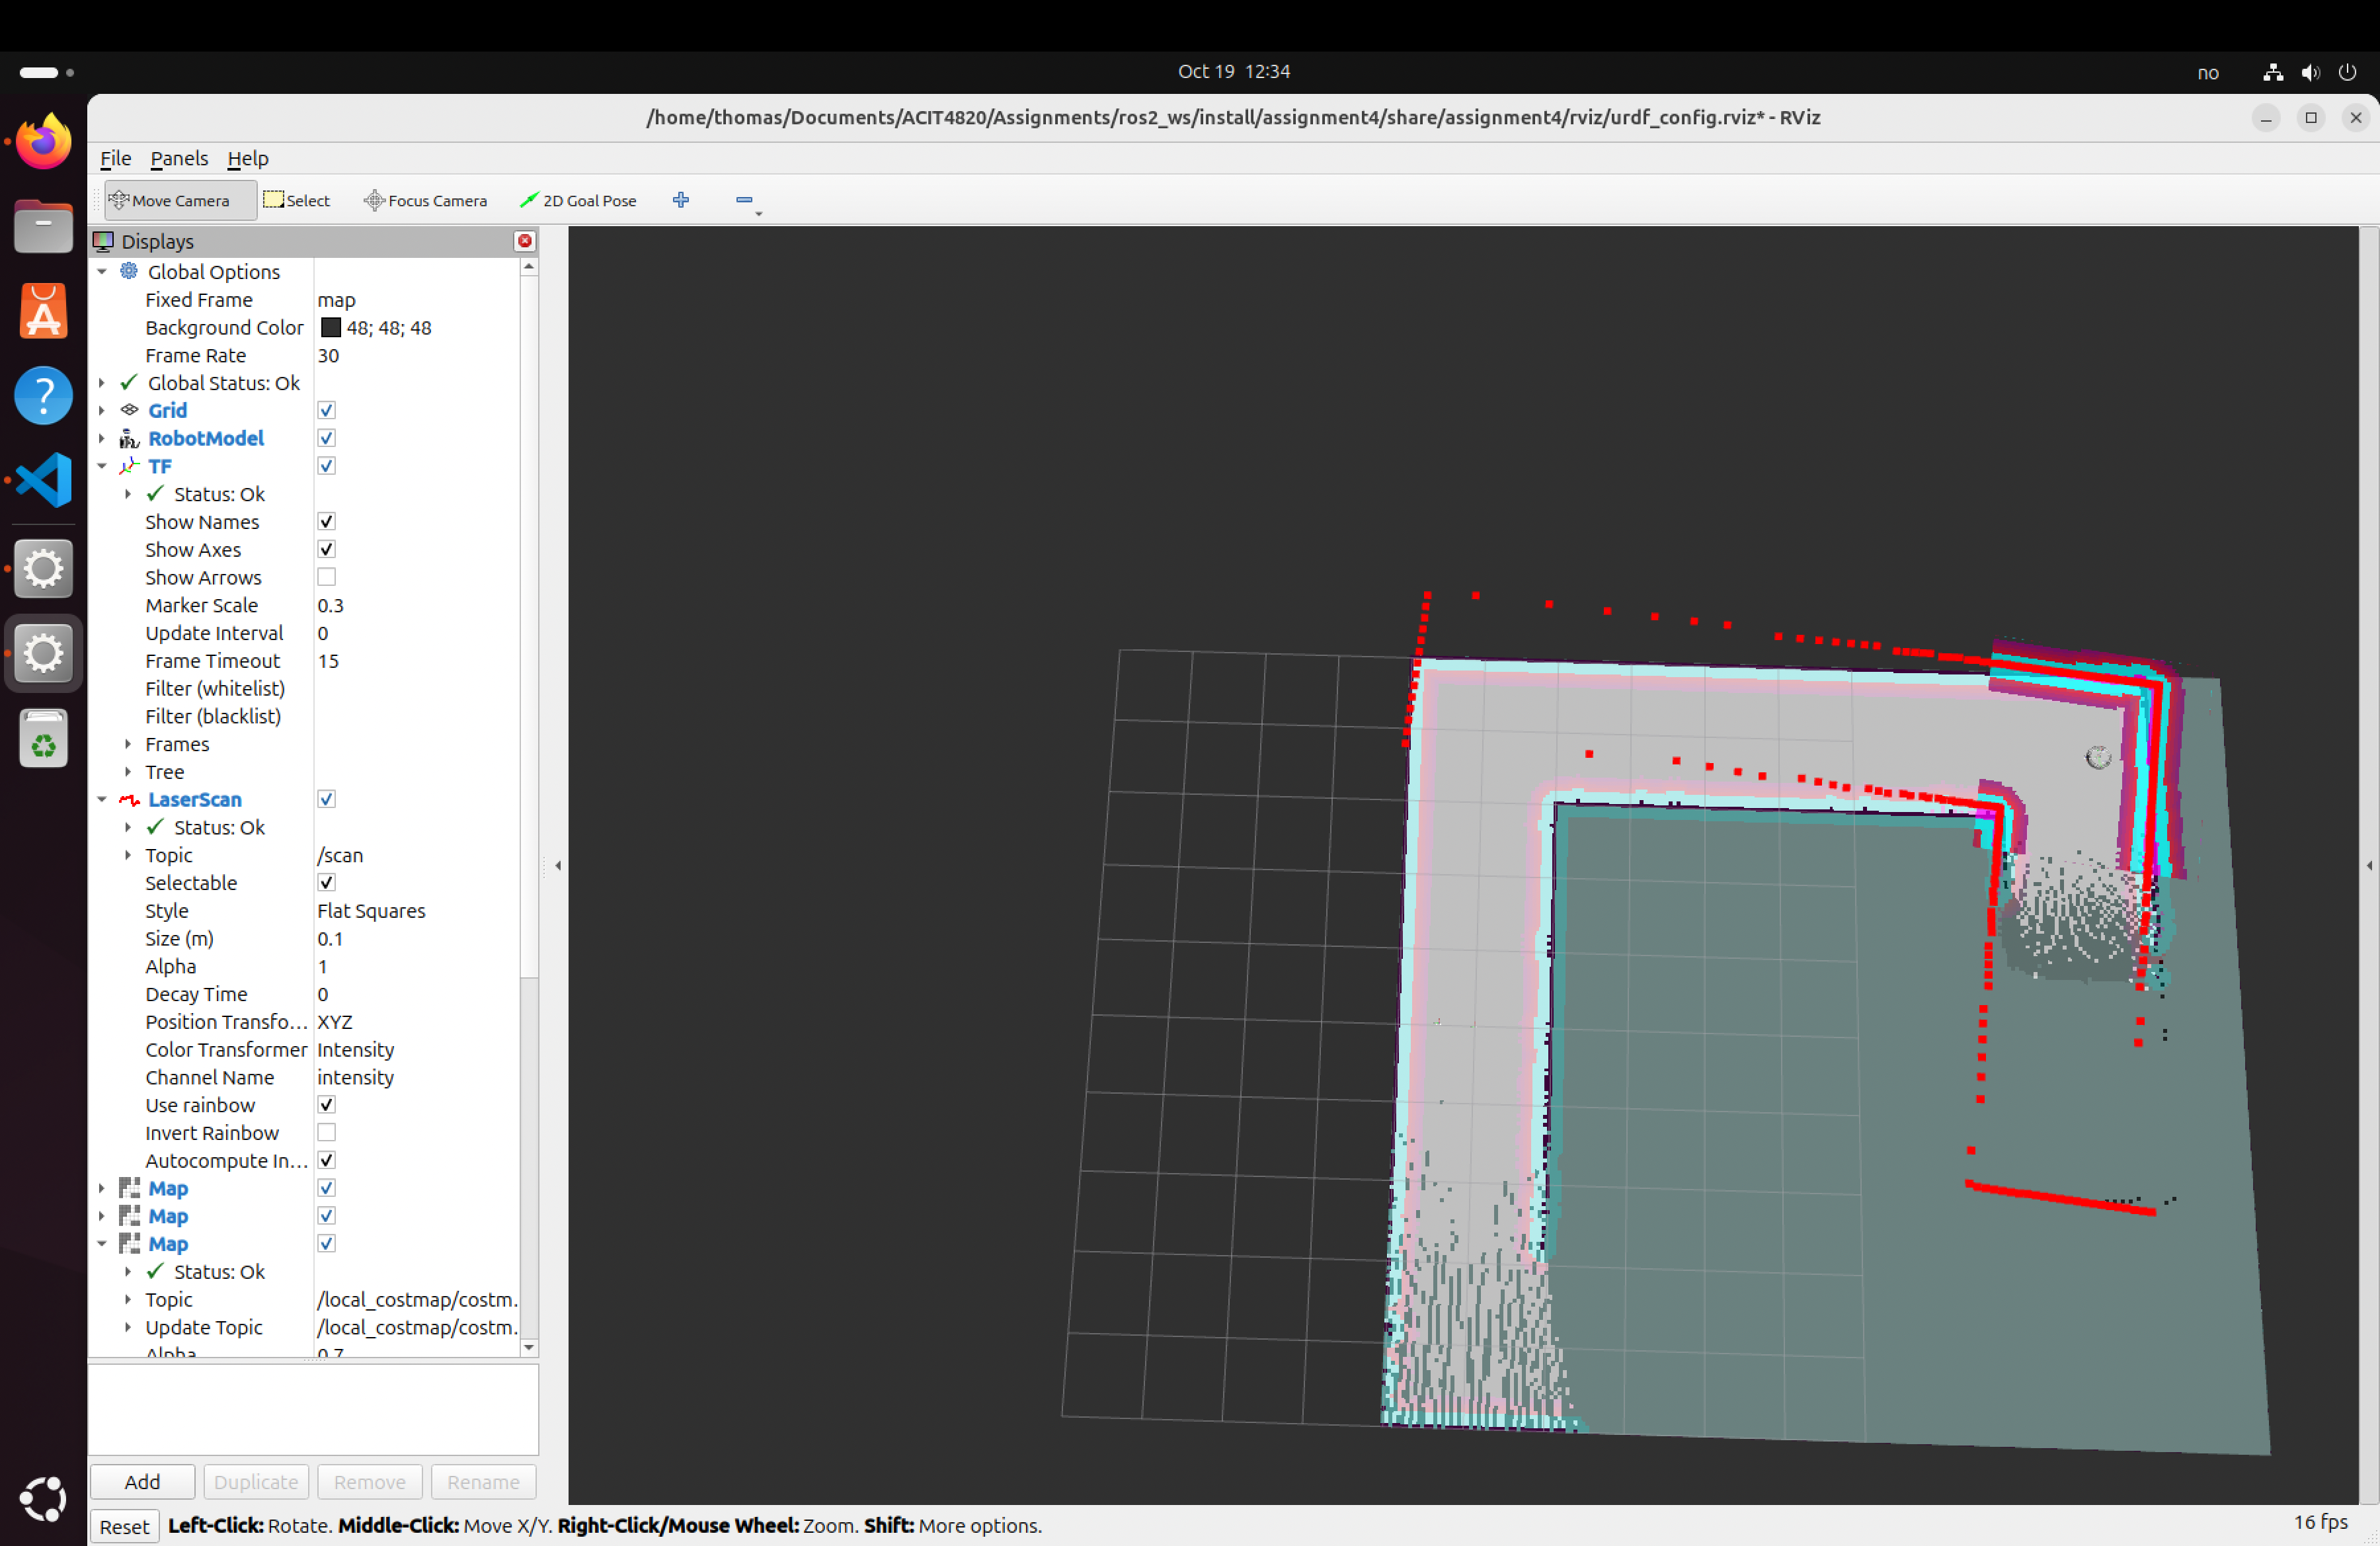
\includegraphics[width=\columnwidth]{fig/04_end.png}
        \caption{End. The top corridor is now mapped.}
    \end{subfigure}
    \caption{Goal 2, around the first corner.}
    \label{fig:goal2}
\end{figure}

\begin{figure}[H]
    \centering
    \begin{subfigure}{\columnwidth}
        \centering
        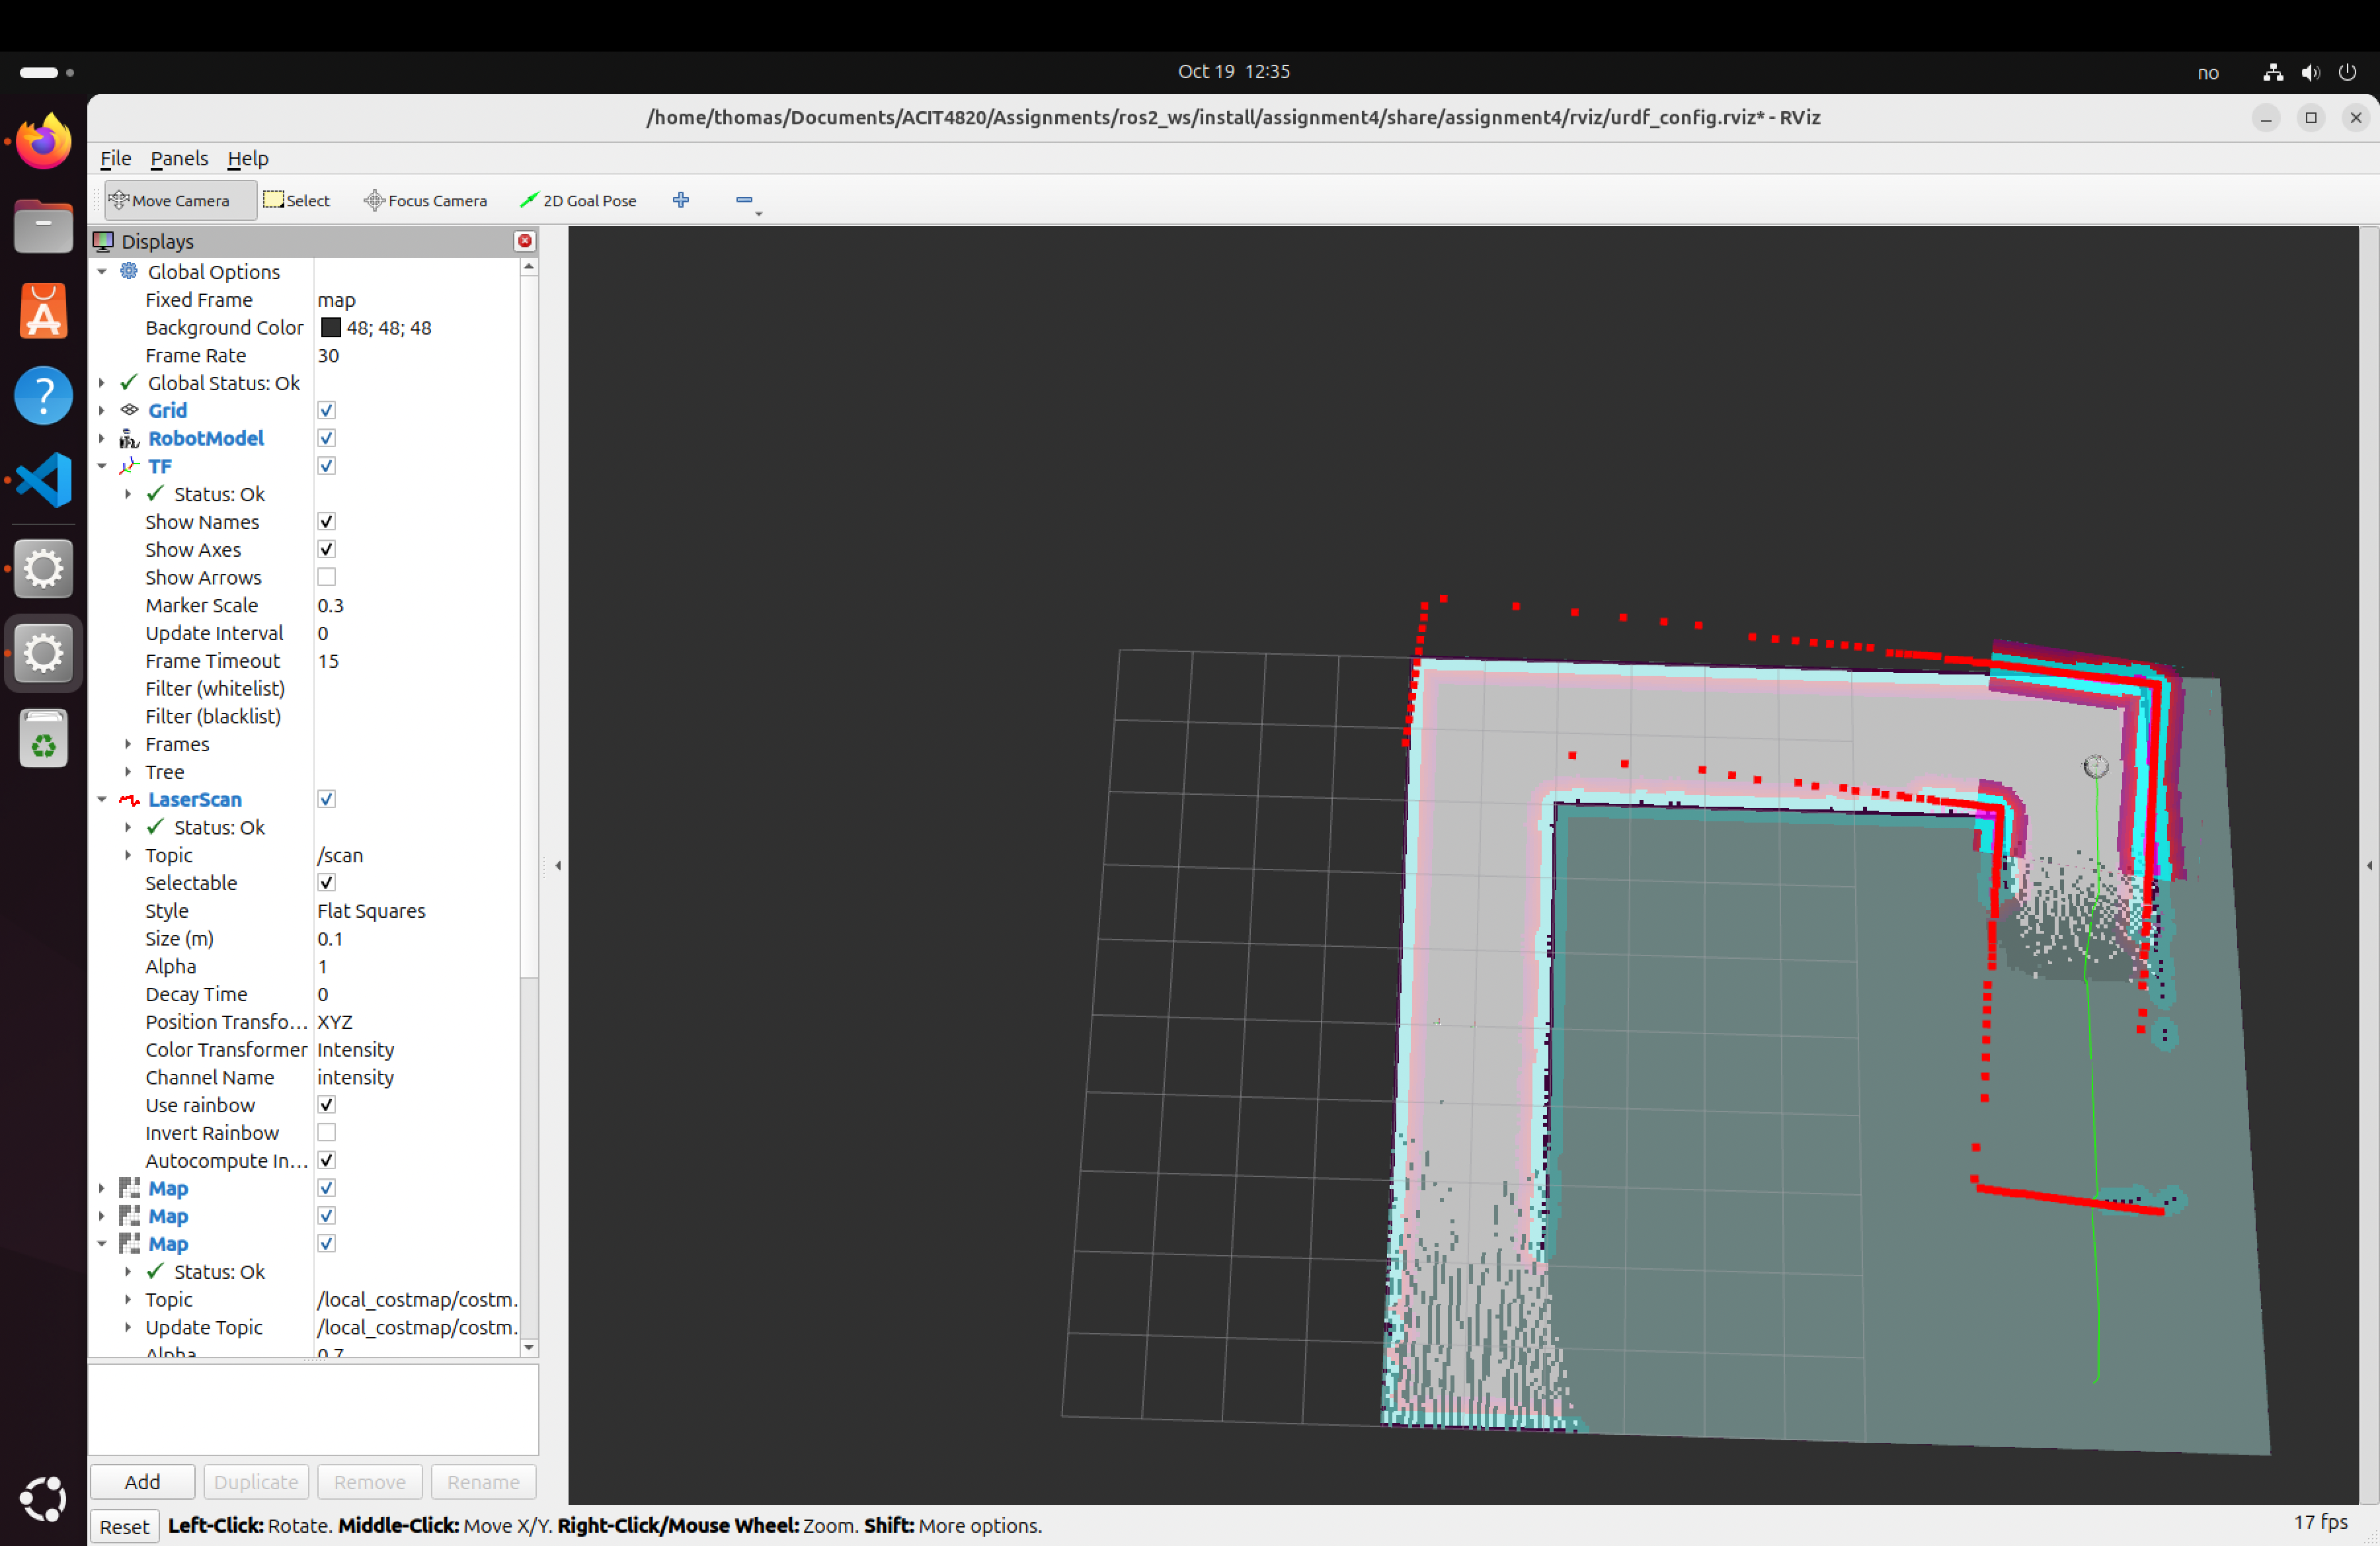
\includegraphics[width=\columnwidth]{fig/05_start.png}
        \caption{Start. The path goes down the right corridor.}
    \end{subfigure}
    \begin{subfigure}{\columnwidth}
        \centering
        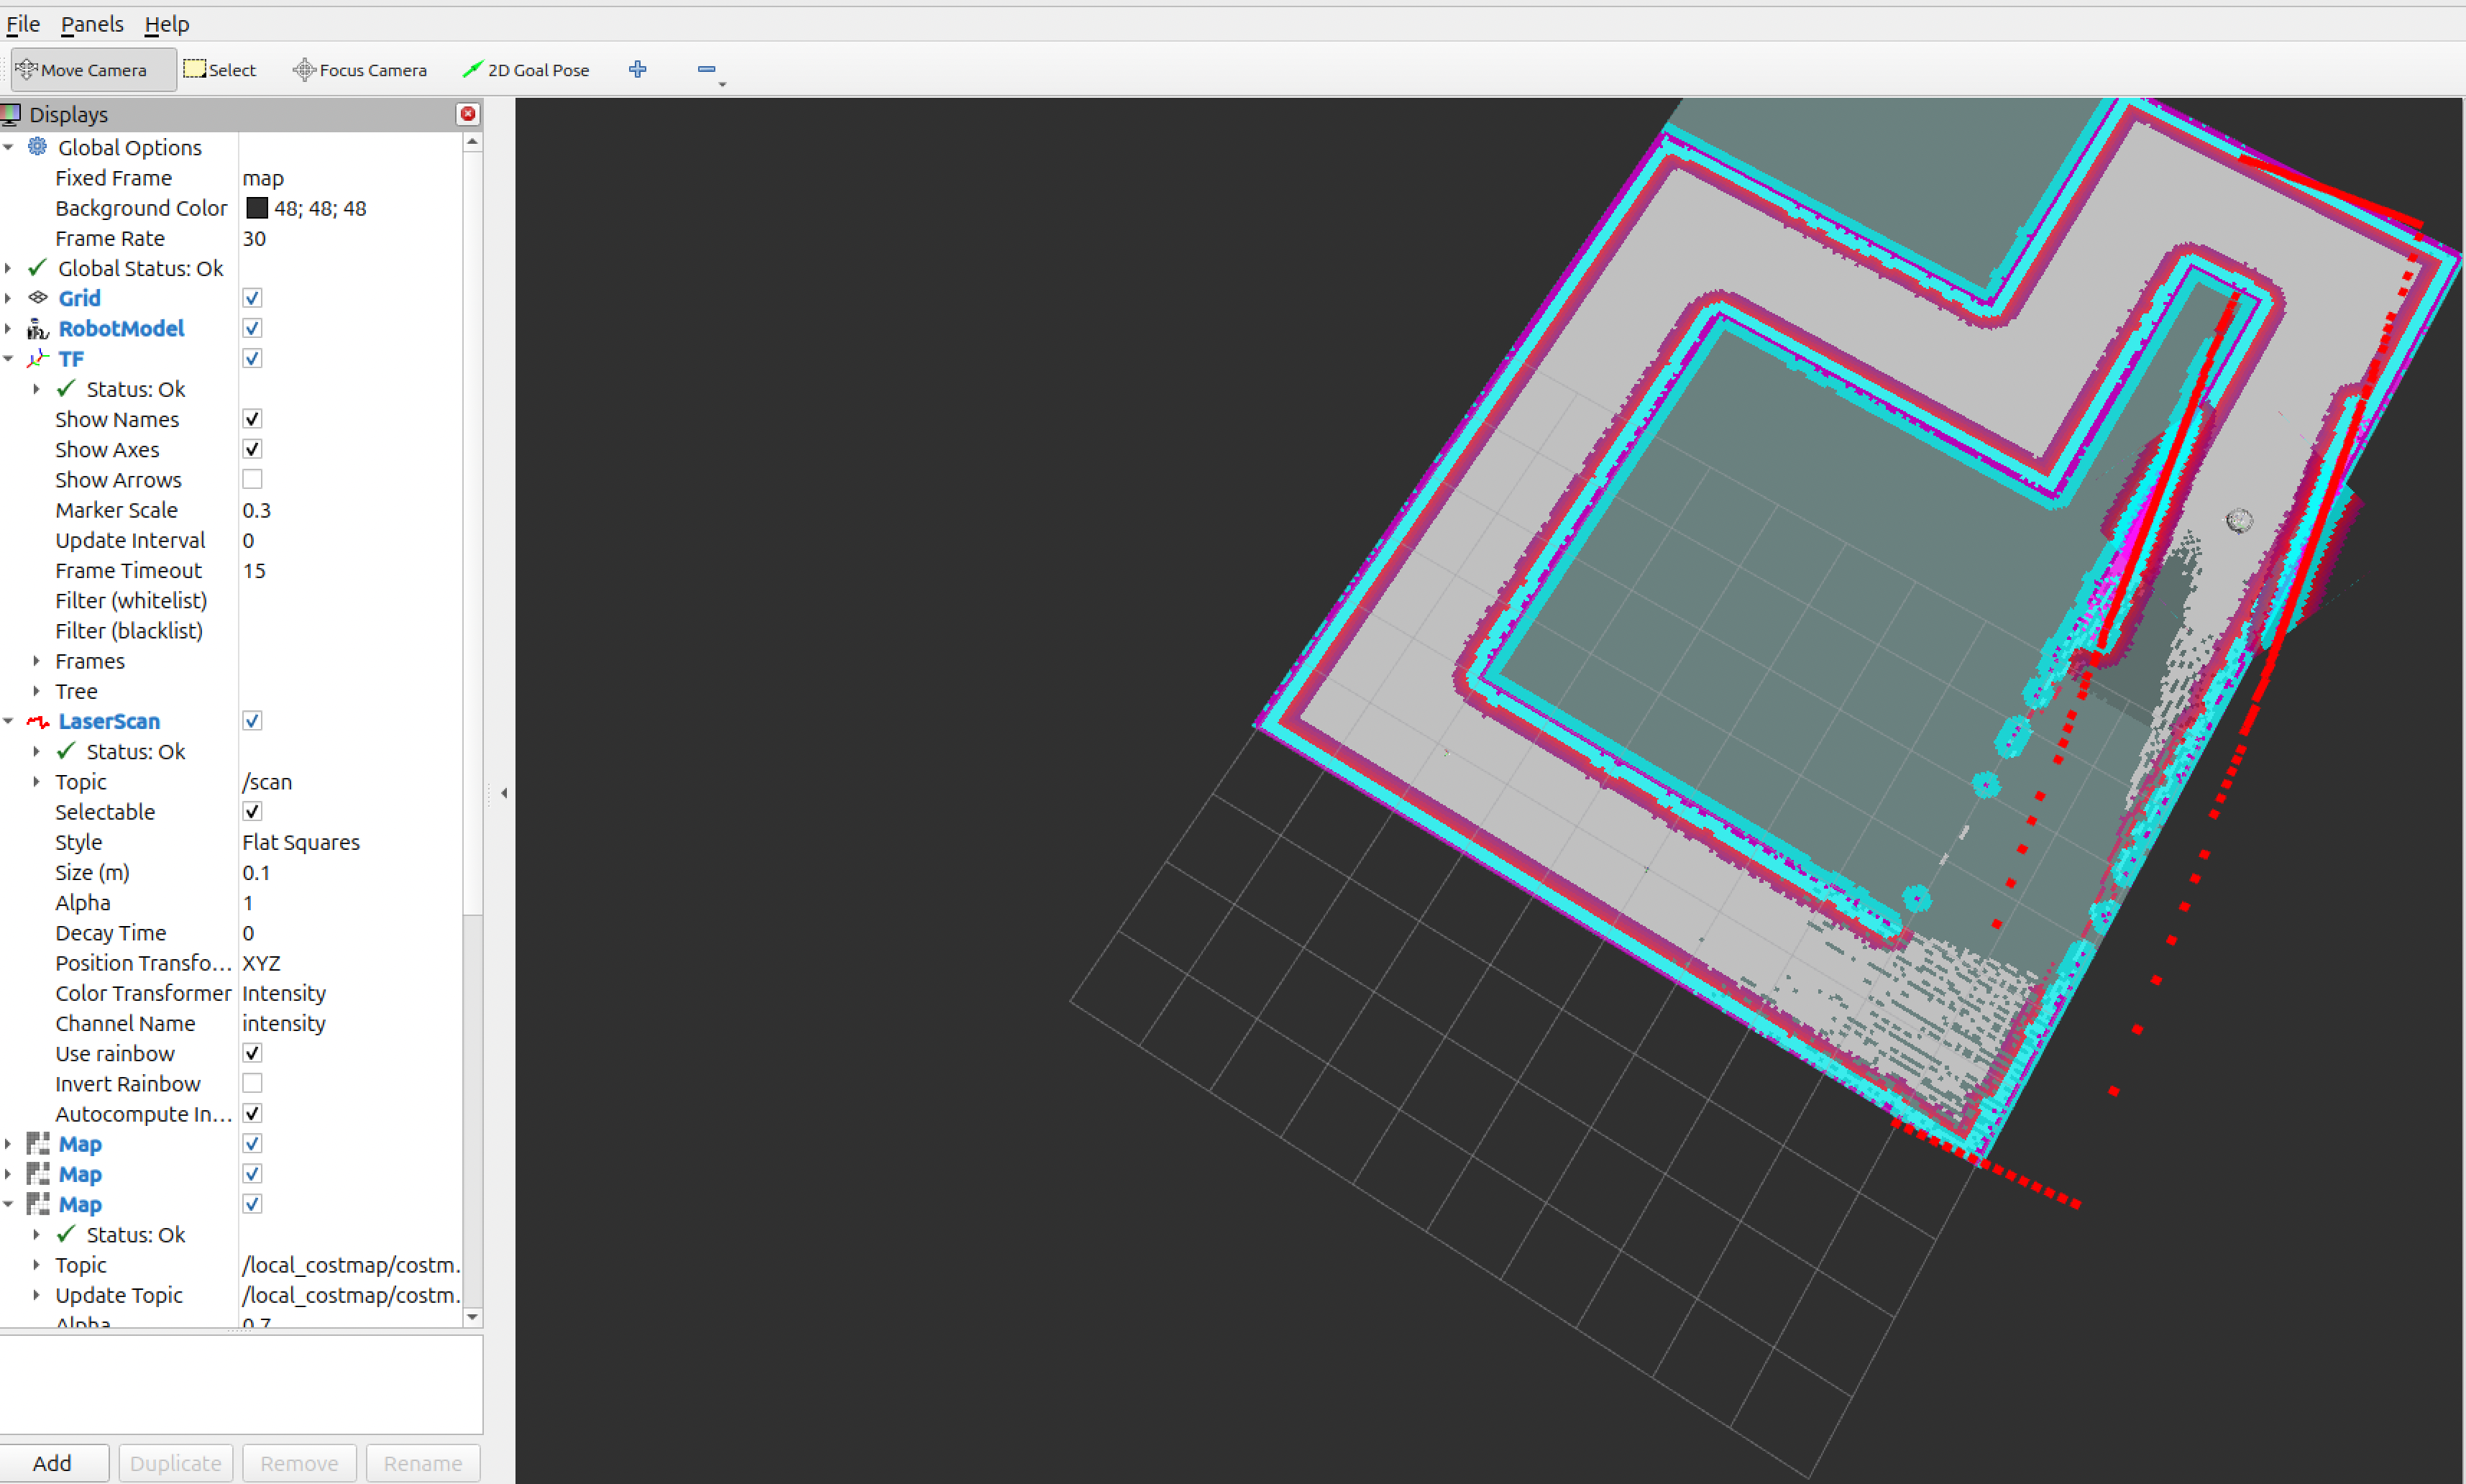
\includegraphics[width=\columnwidth]{fig/06_end.png}
        \caption{End. The walls on the right side are drawn twice.}
    \end{subfigure}
    \caption{Goal 3, down the right corridor.}
    \label{fig:goal3}
\end{figure}

\begin{figure}[H]
    \centering
    \begin{subfigure}{\columnwidth}
        \centering
        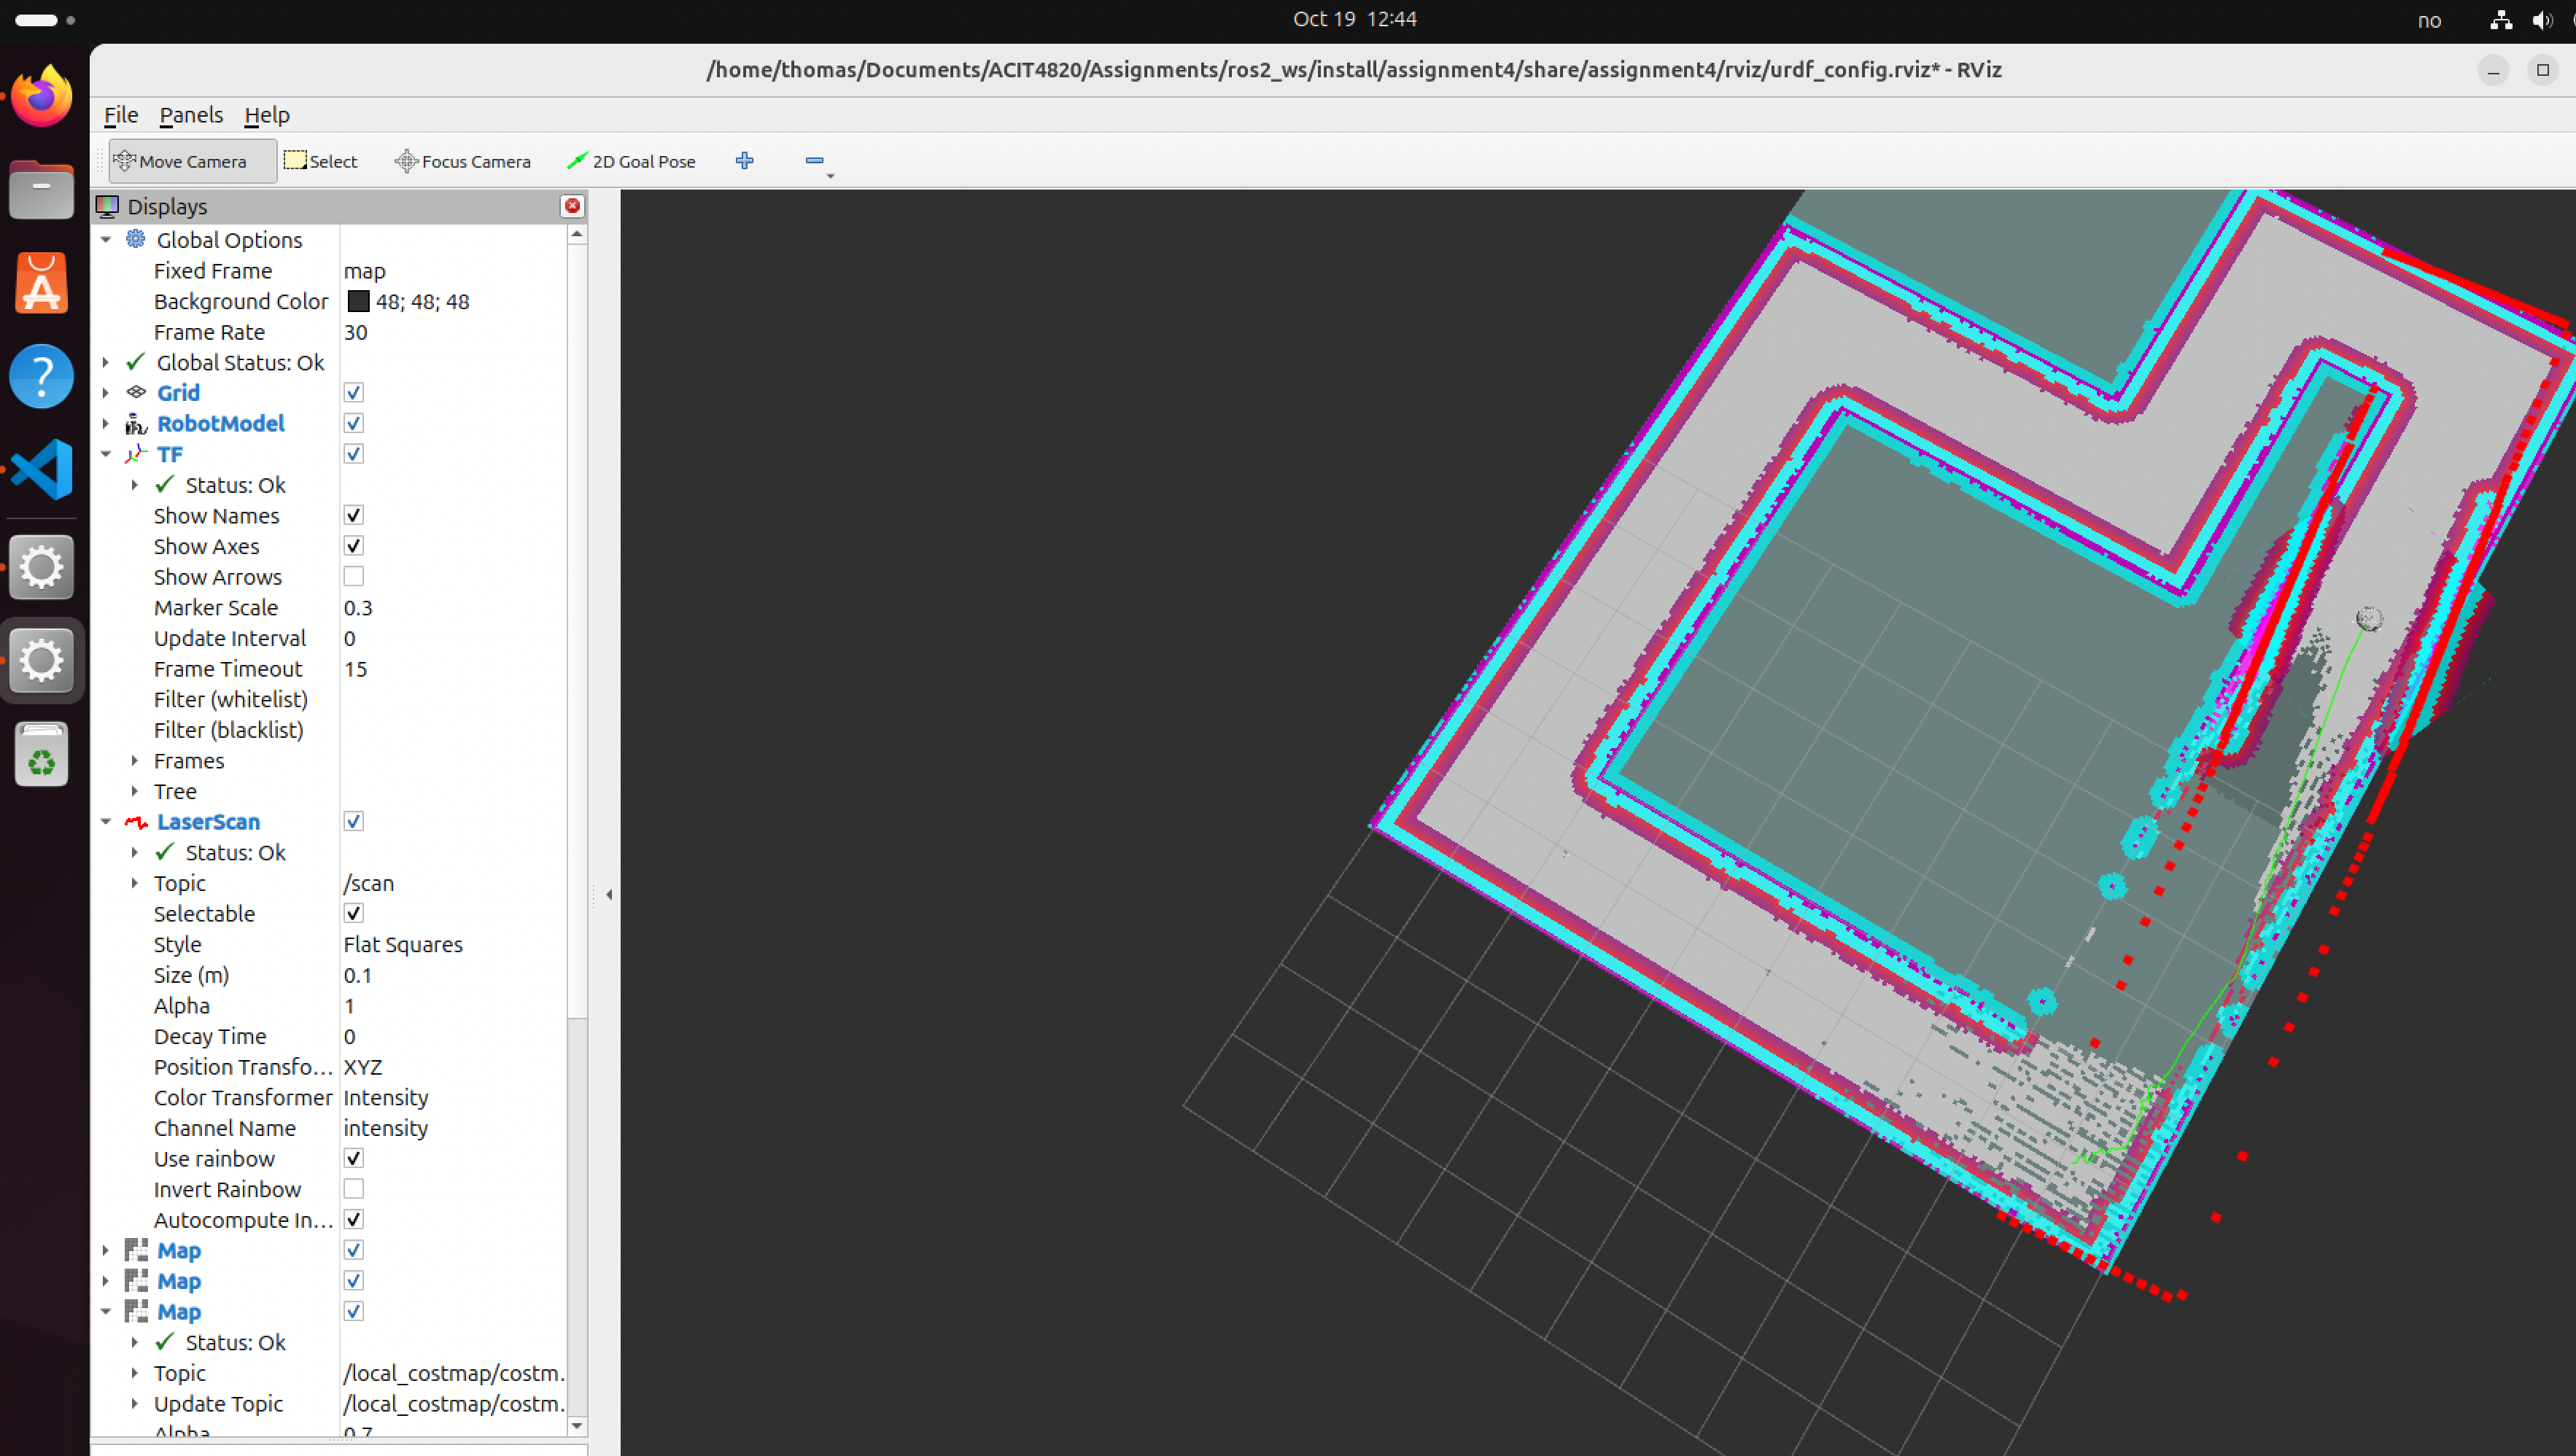
\includegraphics[width=\columnwidth]{fig/07_start.png}
        \caption{Start. The path follows the right corridor back down.}
    \end{subfigure}
    \begin{subfigure}{\columnwidth}
        \centering
        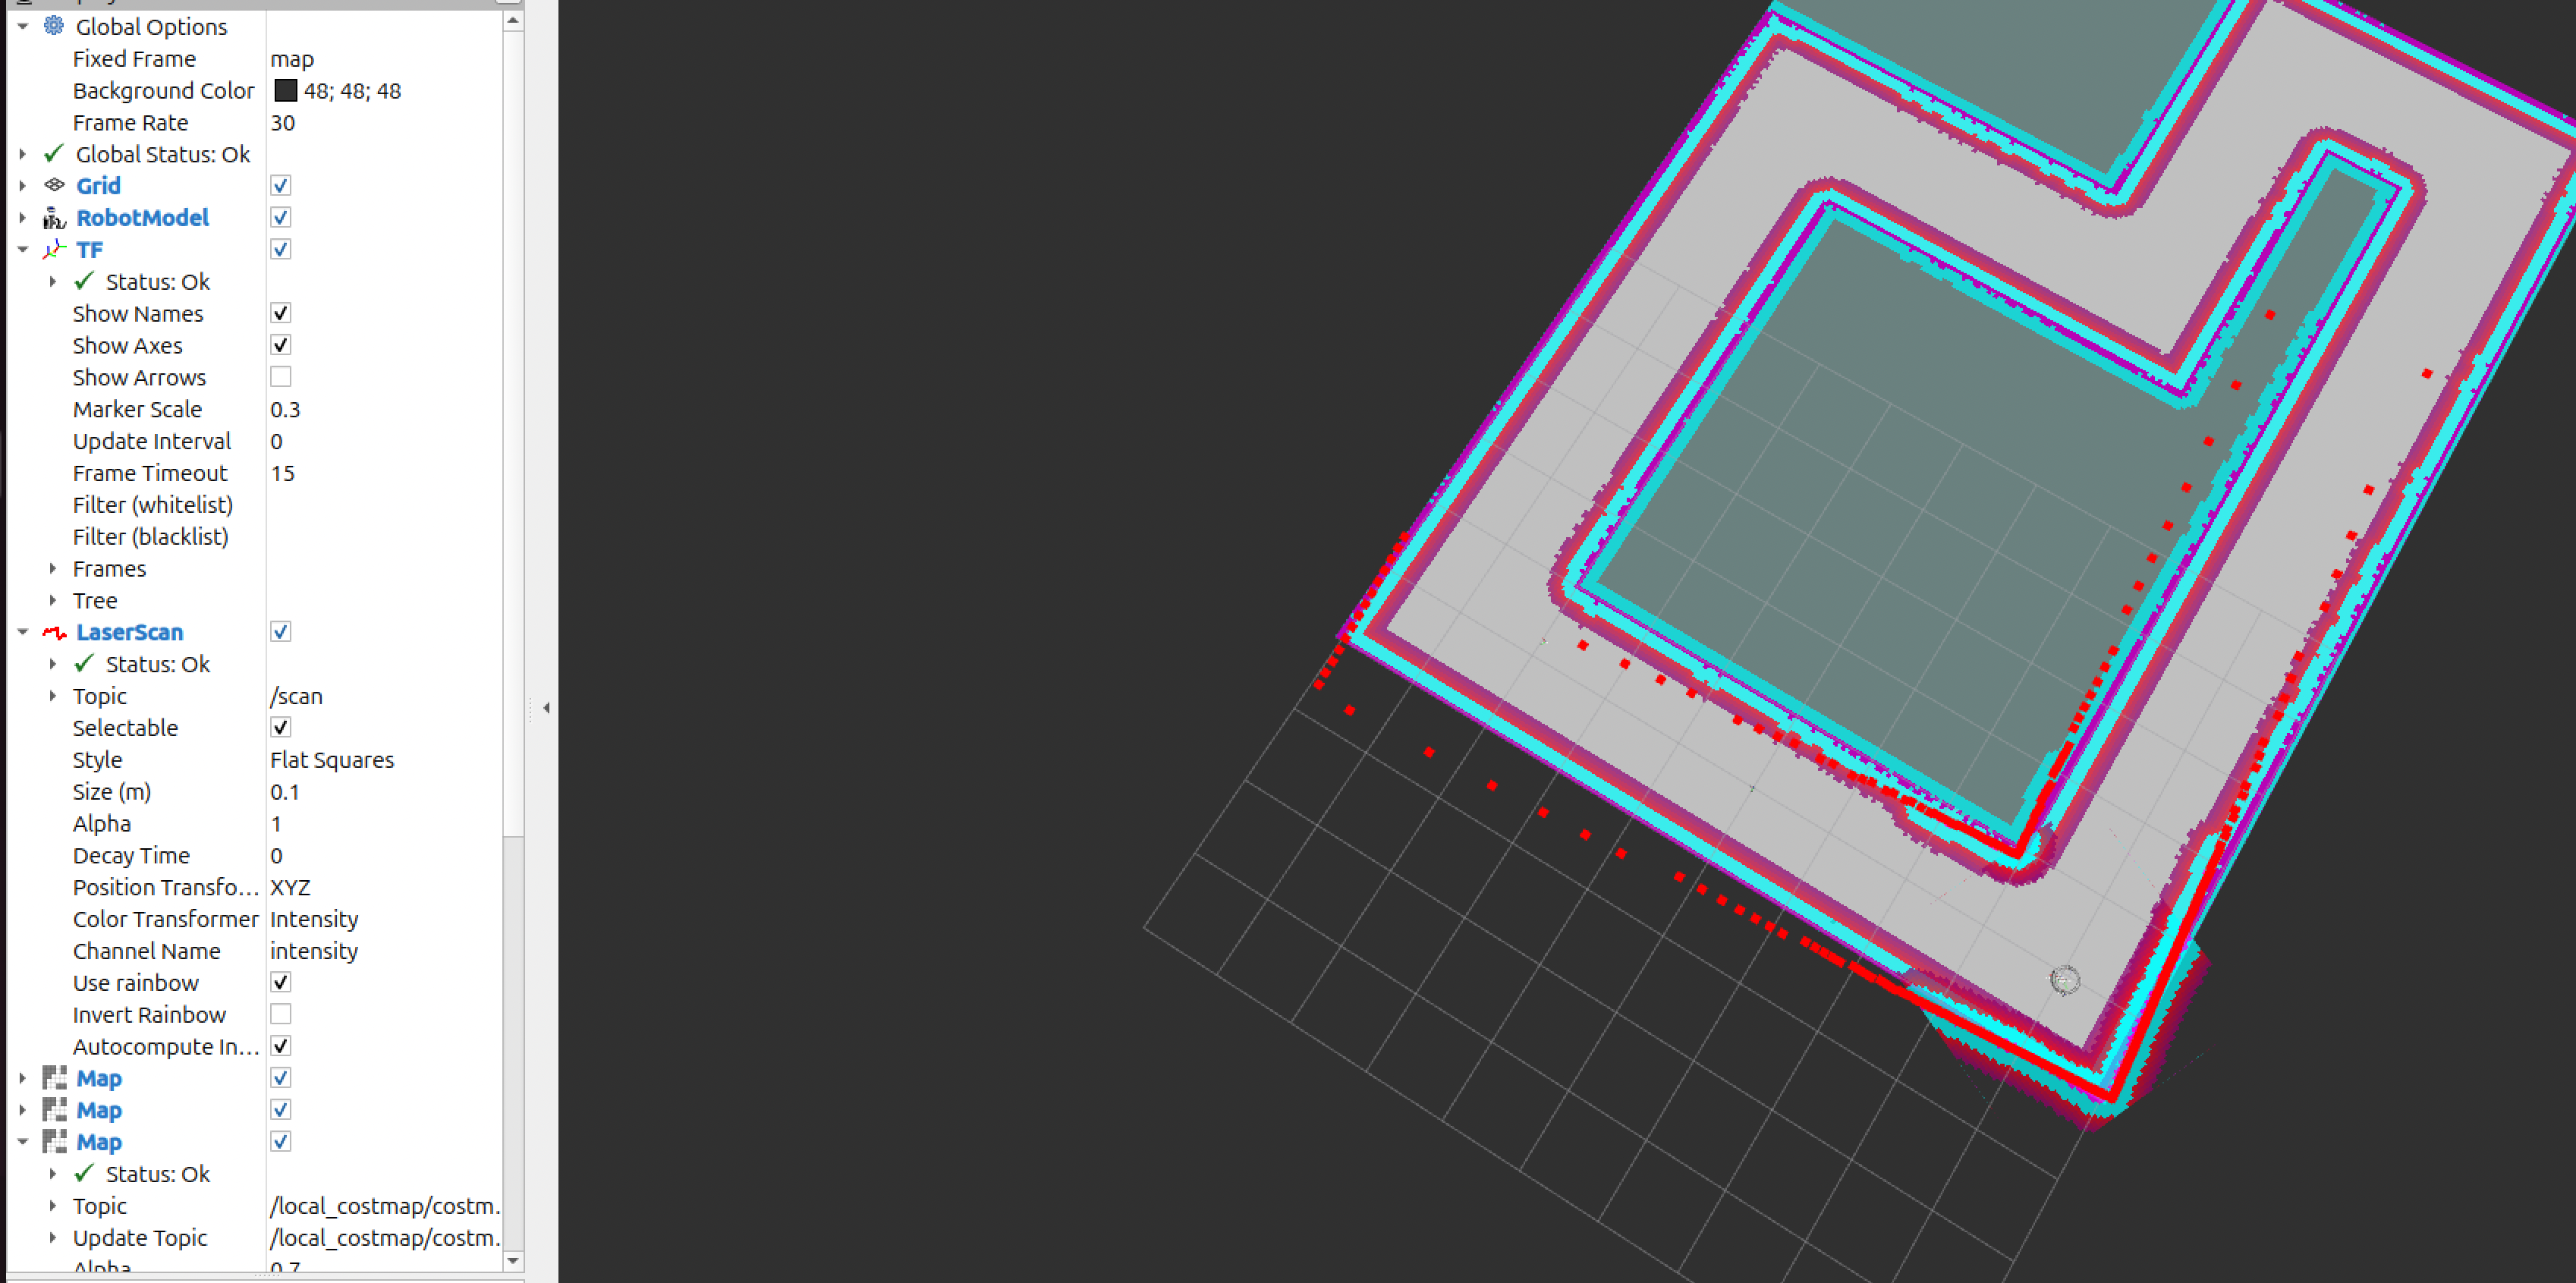
\includegraphics[width=\columnwidth]{fig/08_end.png}
        \caption{End. Most of the maze is mapped, but the scan on the right
                 does not line up with the map.}
    \end{subfigure}
    \caption{Goal 4, back along the right side of the maze.}
    \label{fig:goal4}
\end{figure}

\subsection{Task 3}
We started the launch file with \texttt{explore:=true} and let the robot drive
on its own. Fig.~\ref{fig:explore1} and Fig.~\ref{fig:explore2} show the
exploration from start to end. We did not send any goals. The green line is
the path to the frontier the explorer chose.

\begin{figure}[H]
    \centering
    \begin{subfigure}{\columnwidth}
        \centering
        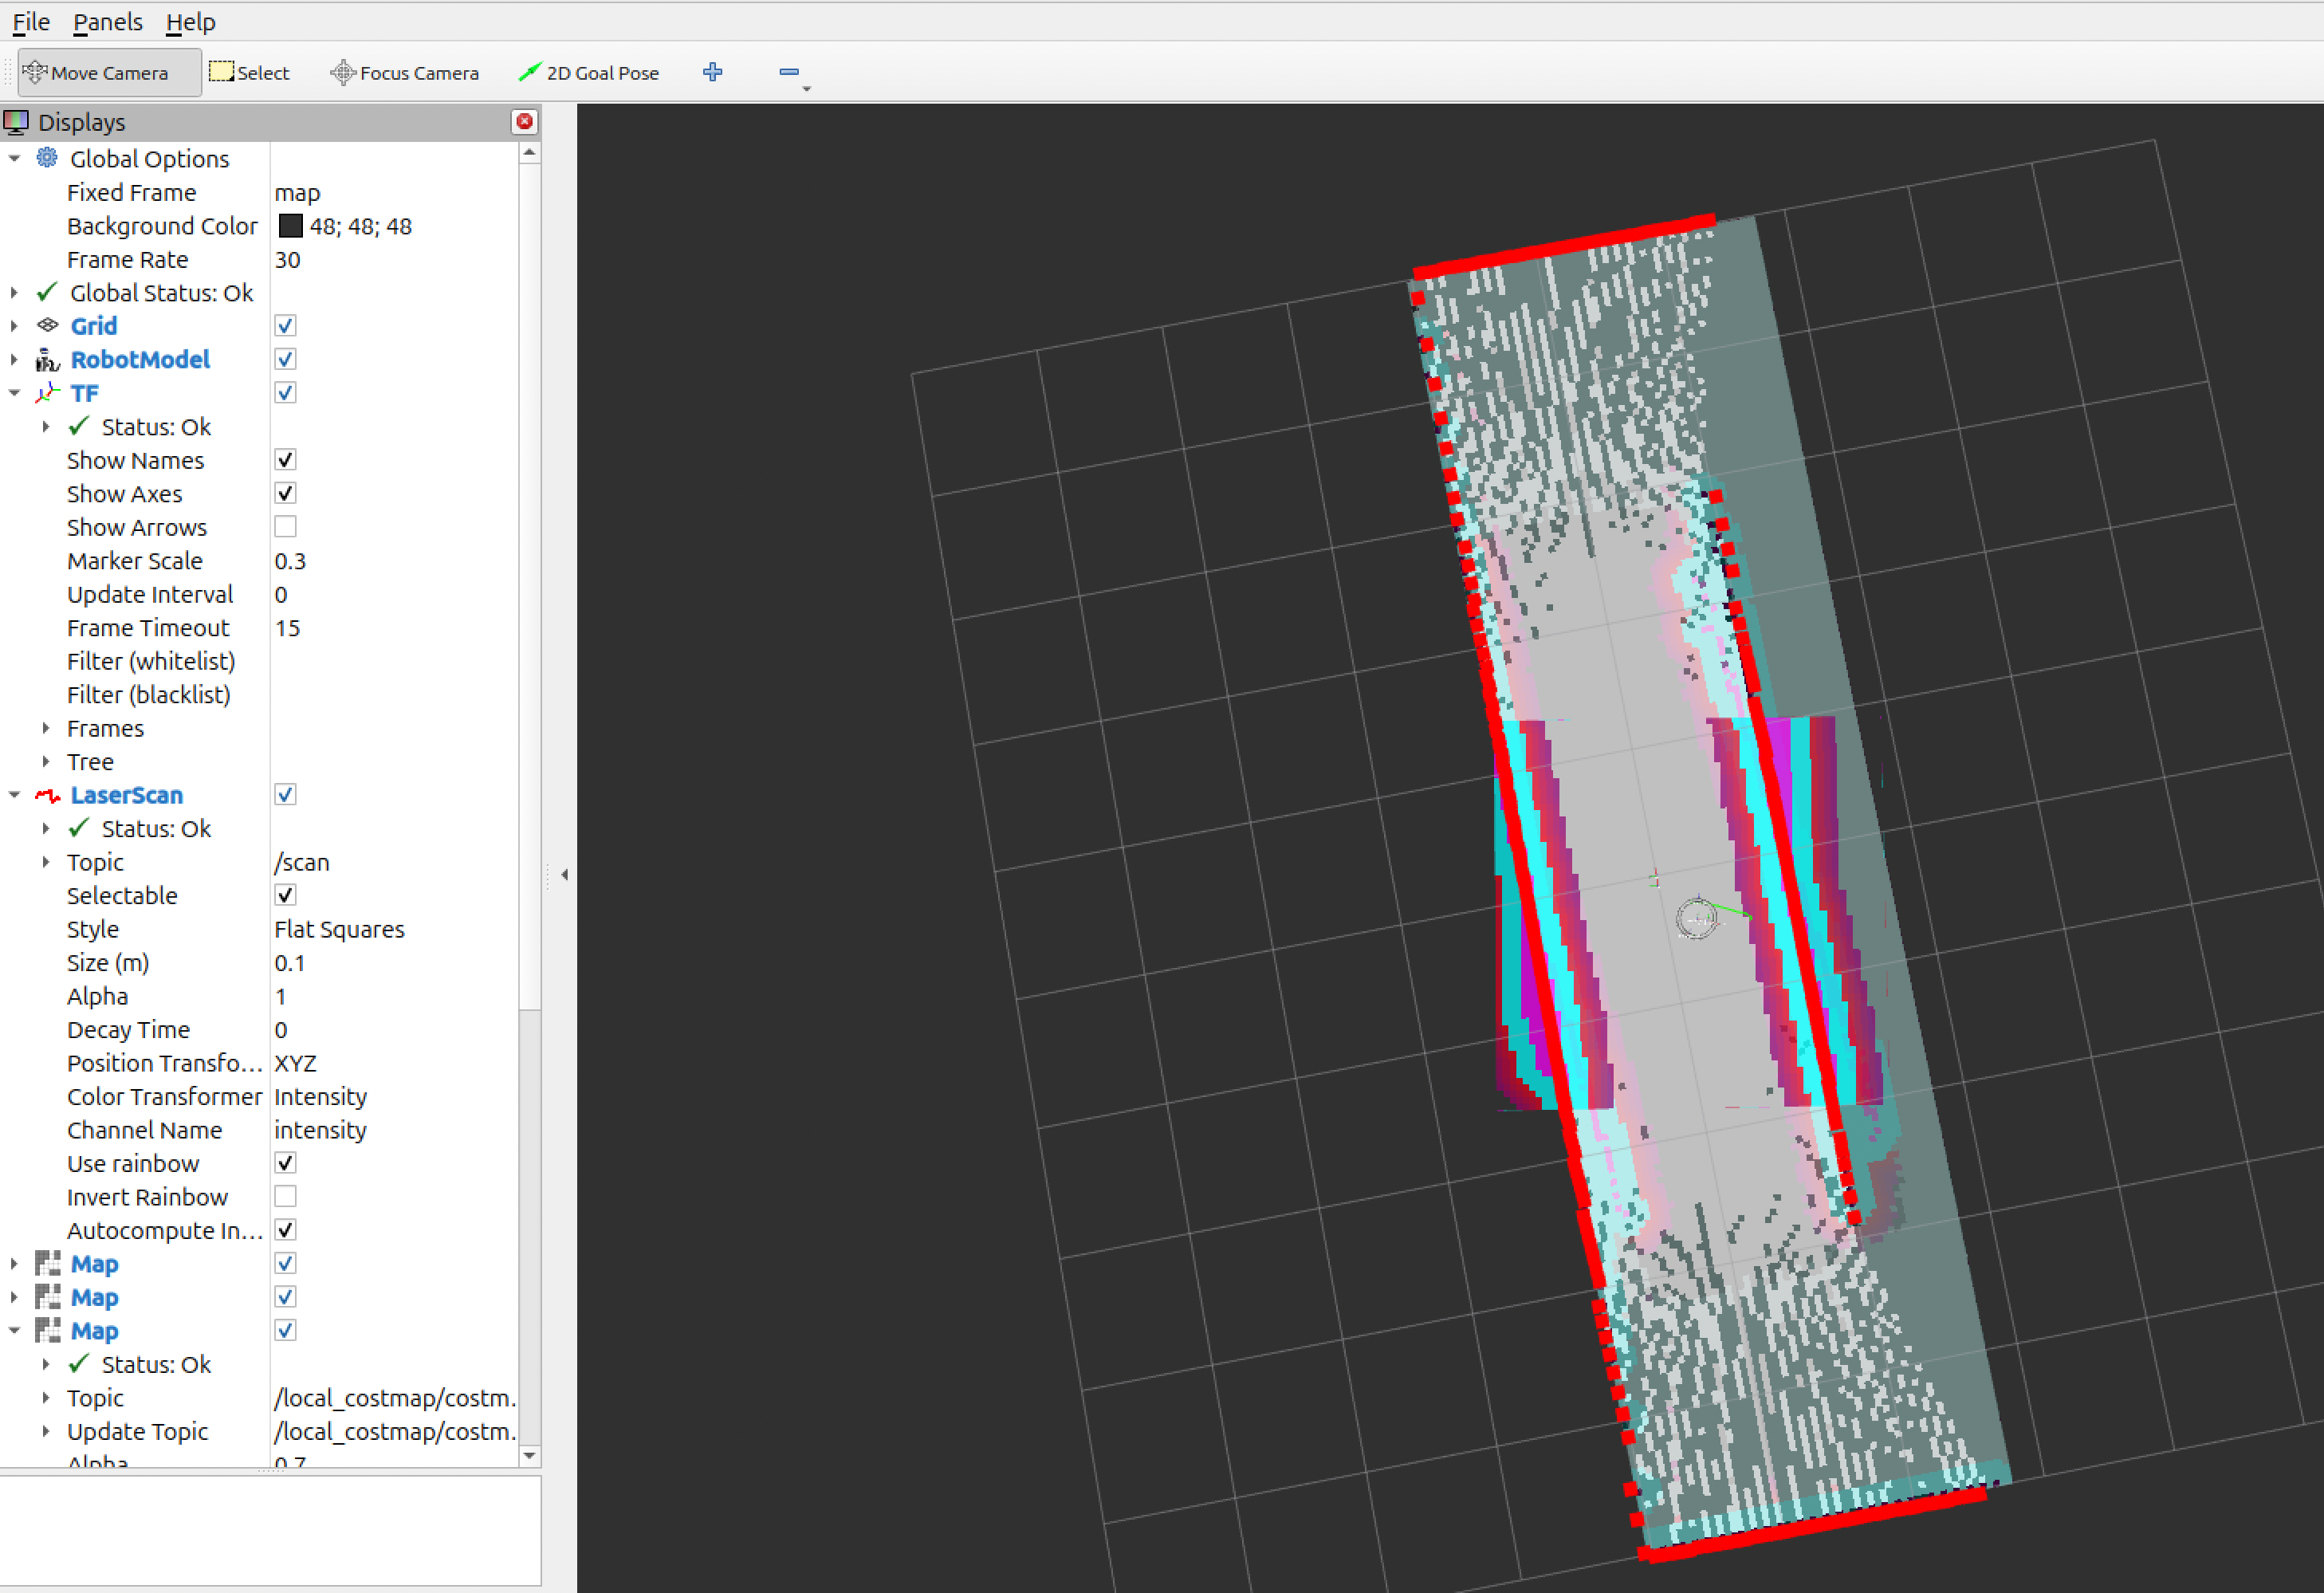
\includegraphics[width=\columnwidth]{fig/09_image.png}
        \caption{Start. Only the first corridor is mapped.}
    \end{subfigure}
    \begin{subfigure}{\columnwidth}
        \centering
        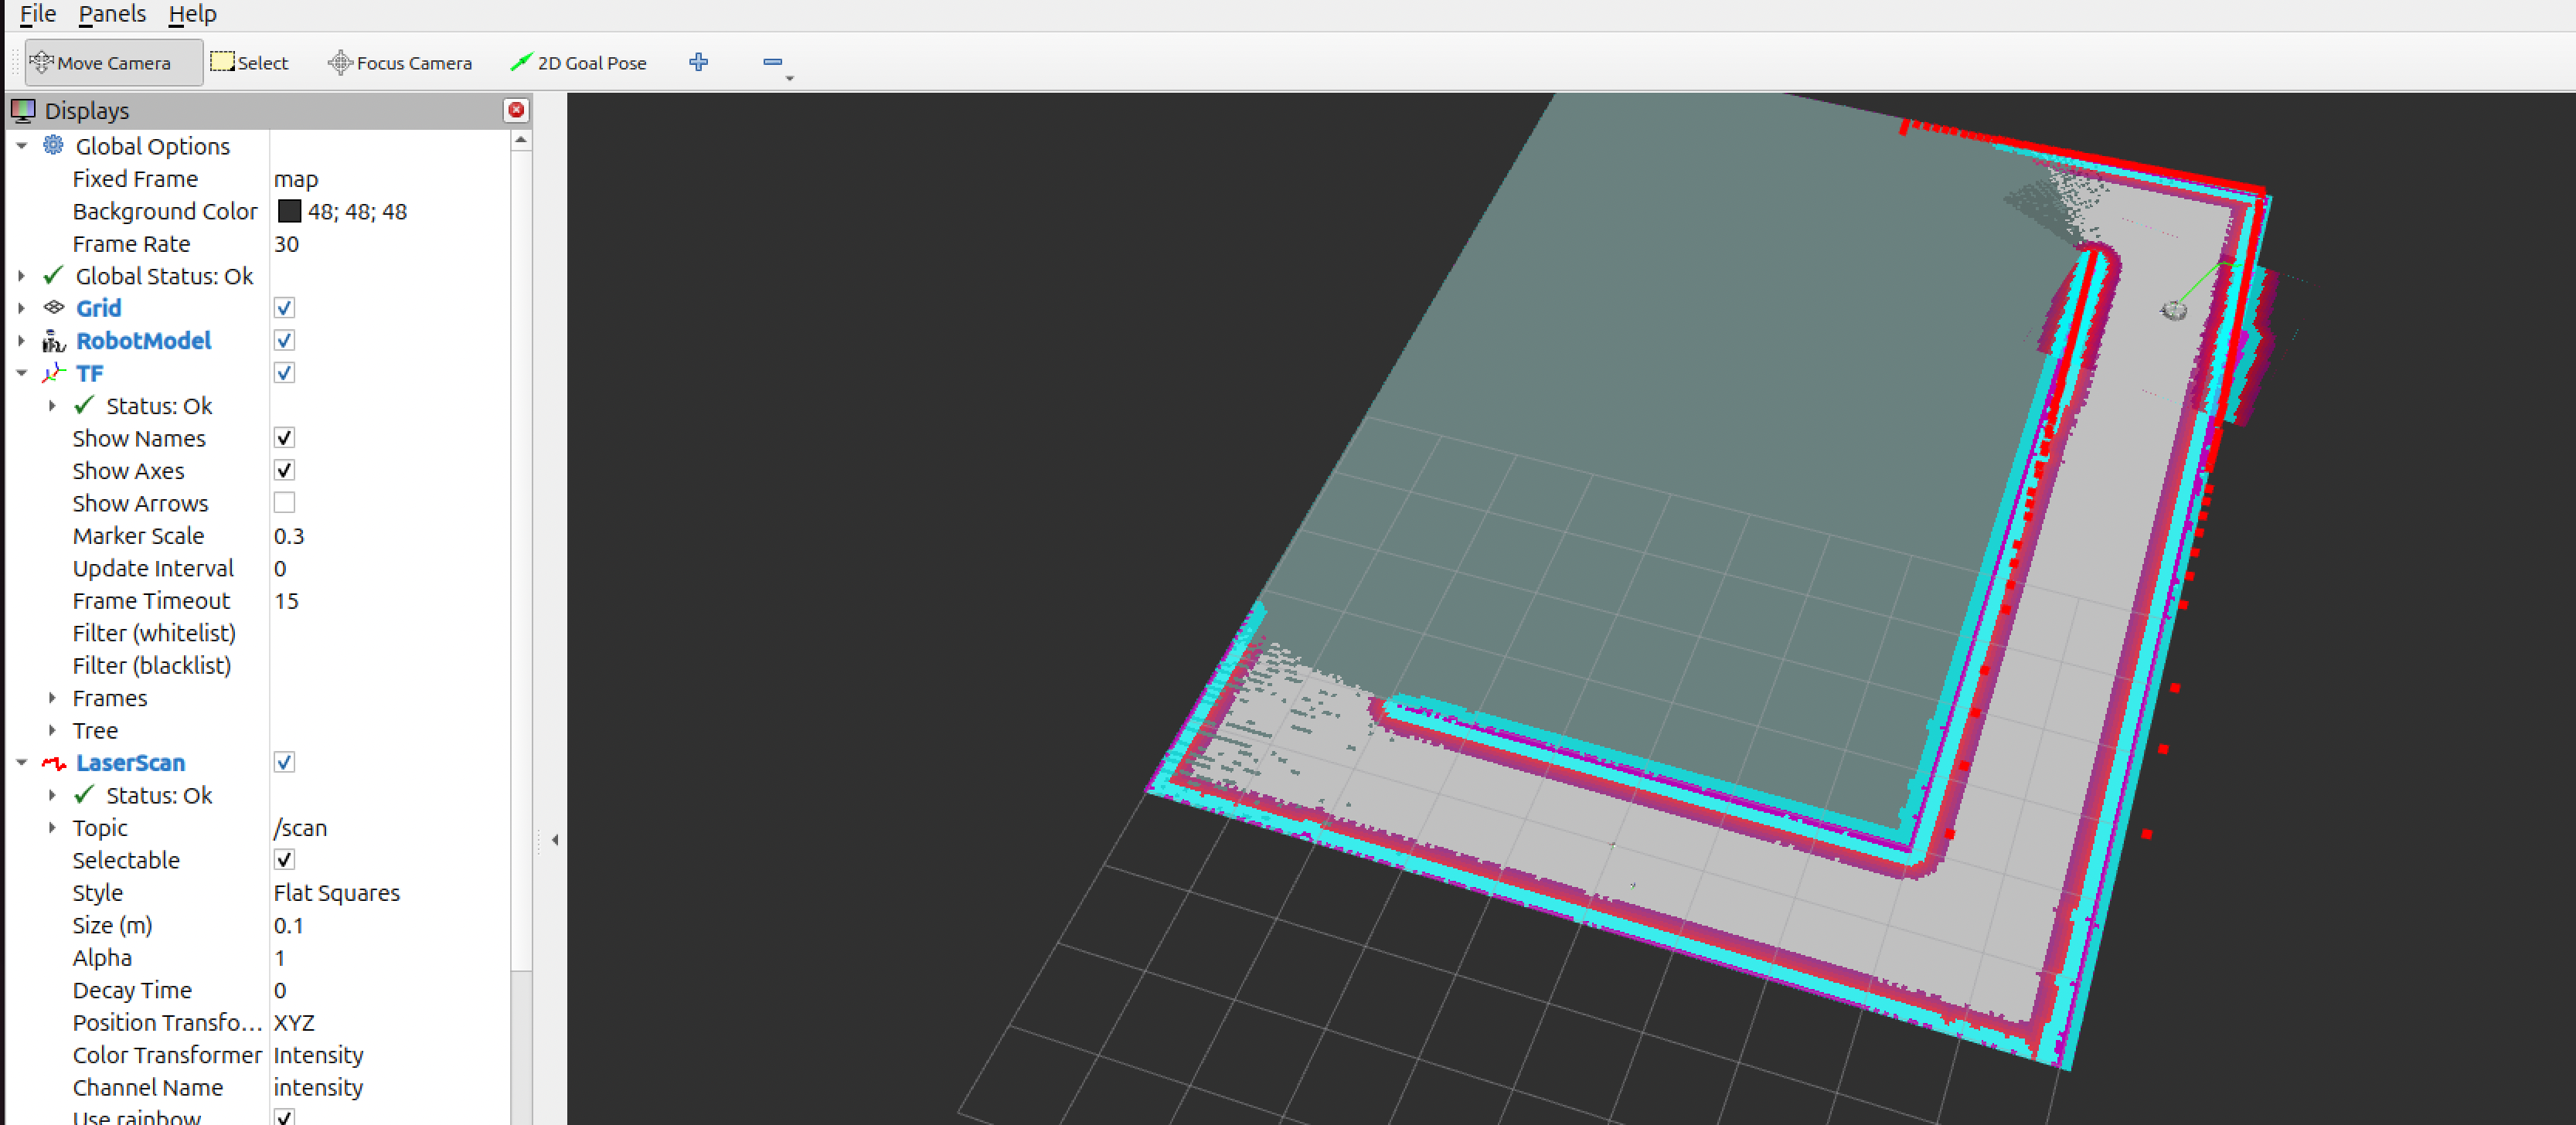
\includegraphics[width=\columnwidth]{fig/10_image.png}
        \caption{The robot has followed the corridor around the first corner.}
    \end{subfigure}
    \caption{The first part of the exploration.}
    \label{fig:explore1}
\end{figure}

\begin{figure}[H]
    \centering
    \begin{subfigure}{\columnwidth}
        \centering
        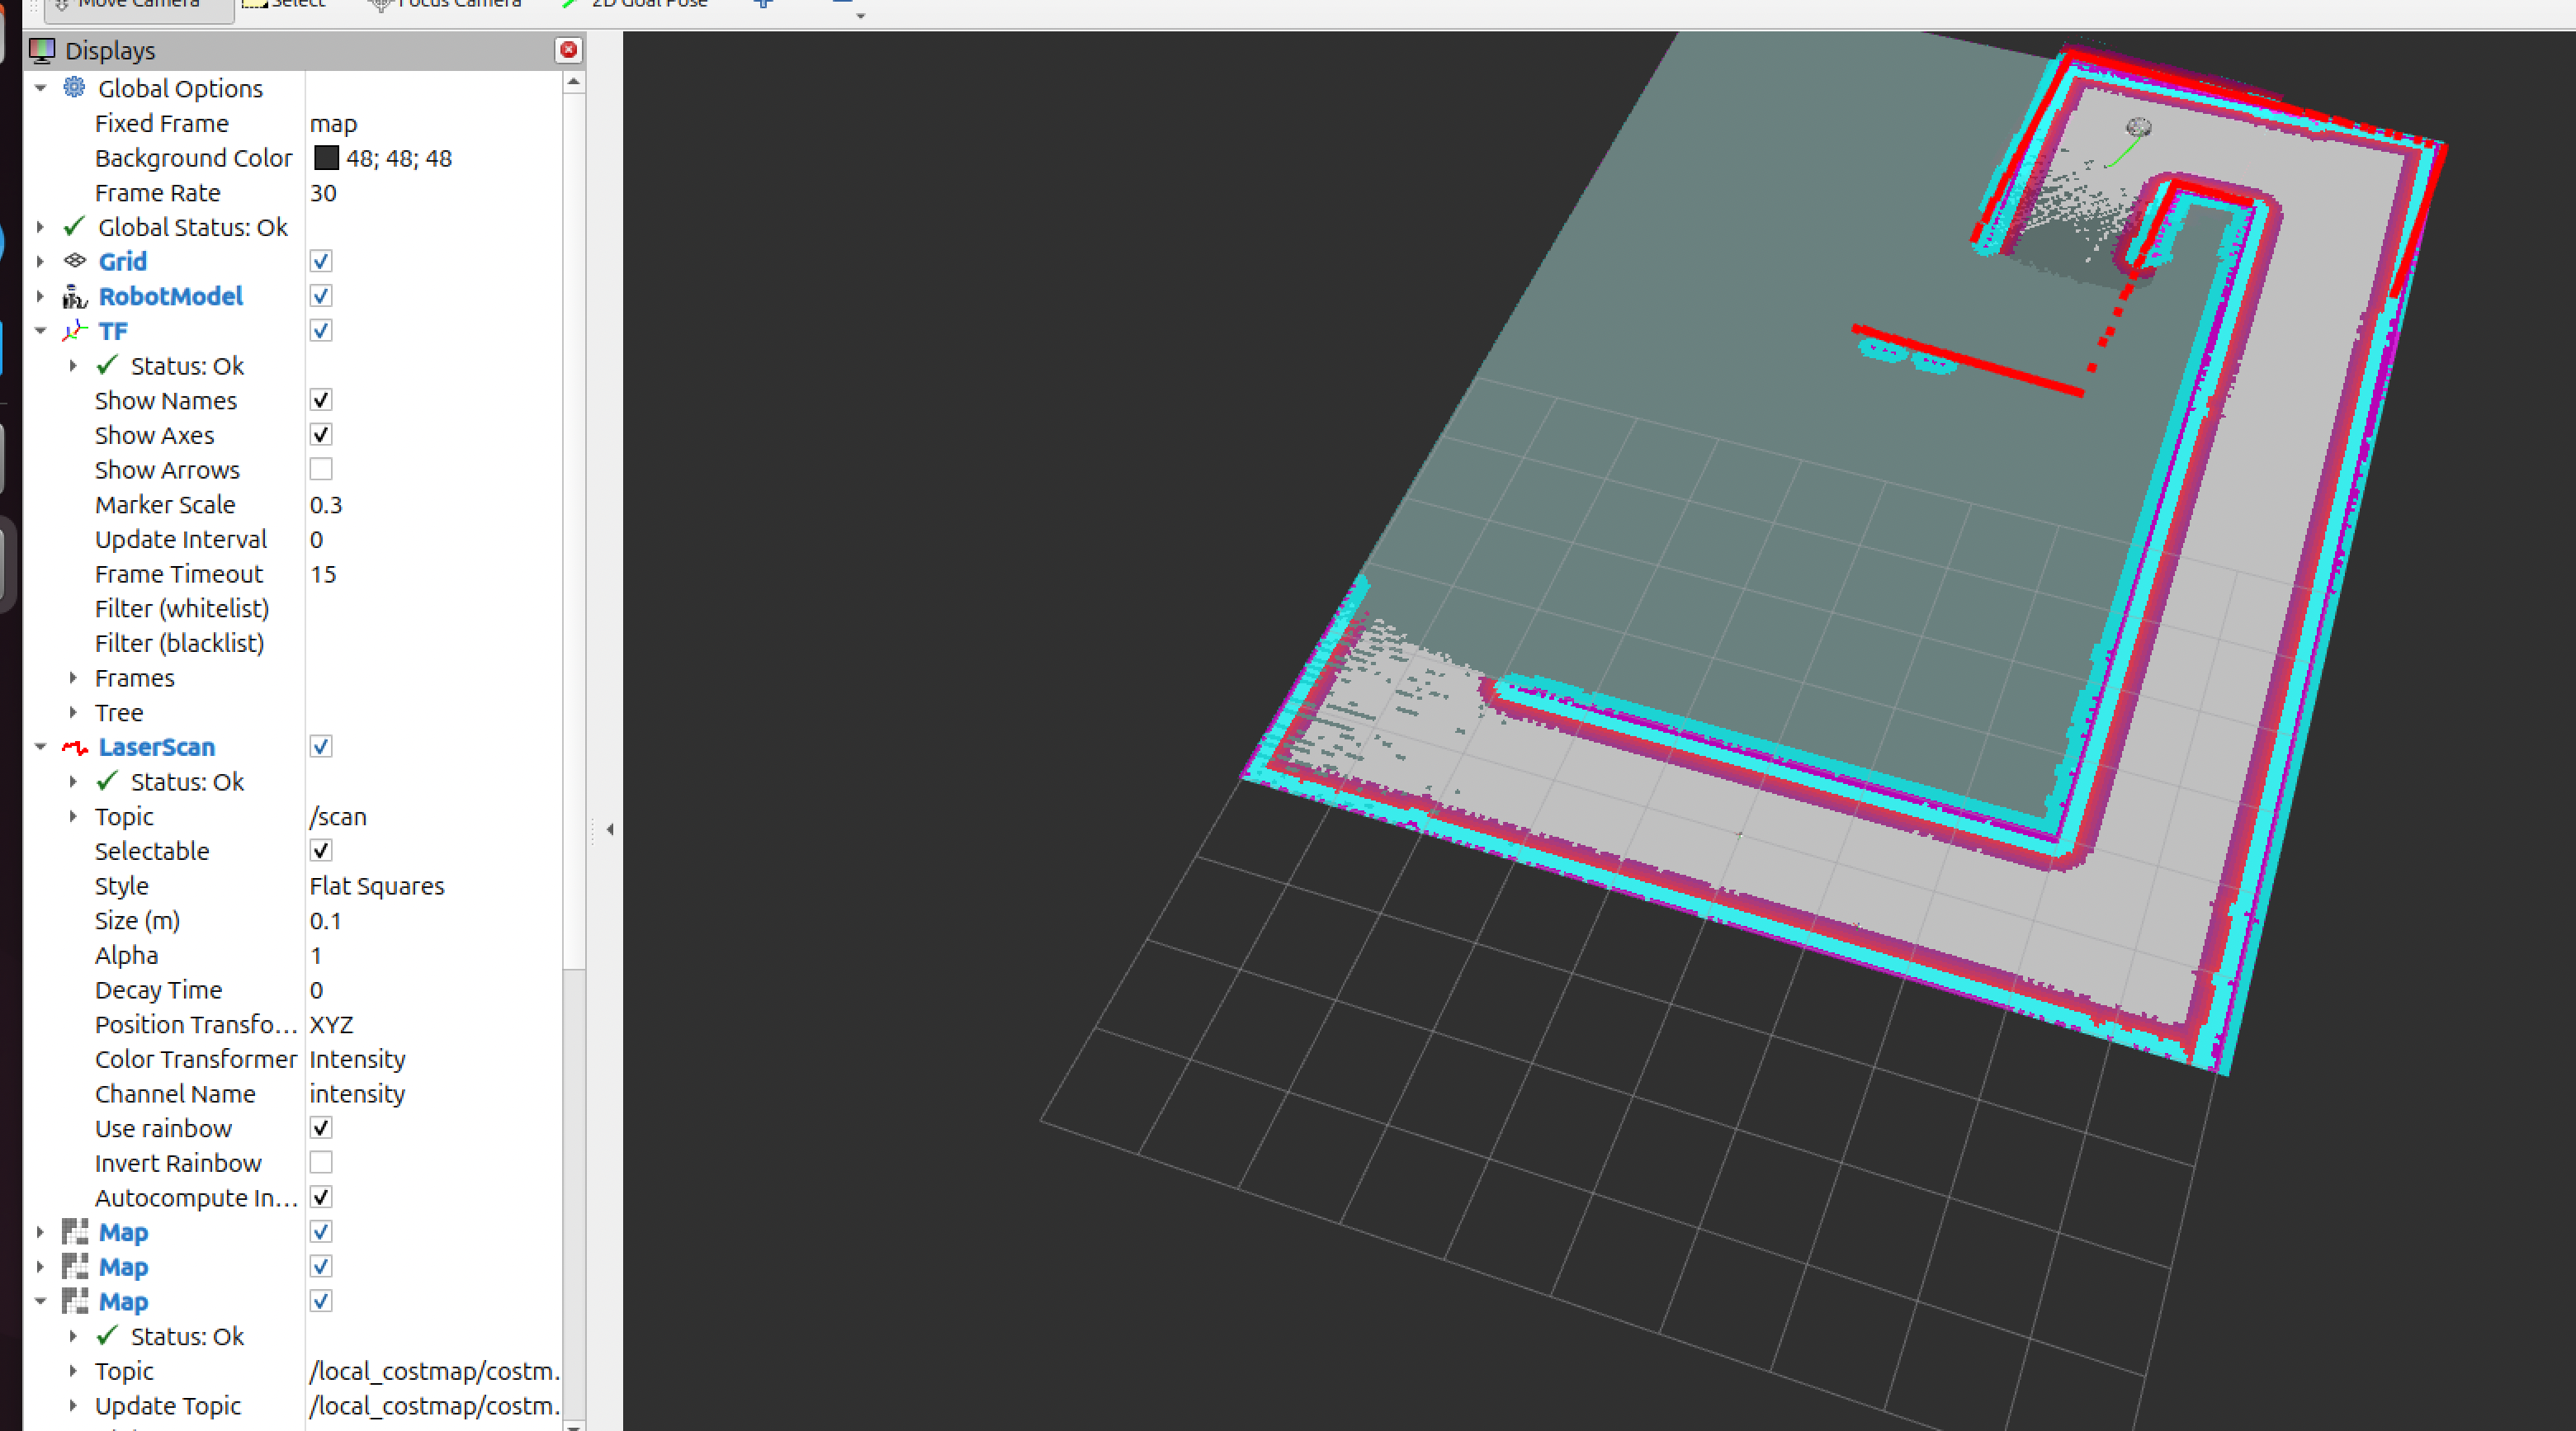
\includegraphics[width=\columnwidth]{fig/11_image.png}
        \caption{The robot is mapping the top of the maze.}
    \end{subfigure}
    \begin{subfigure}{\columnwidth}
        \centering
        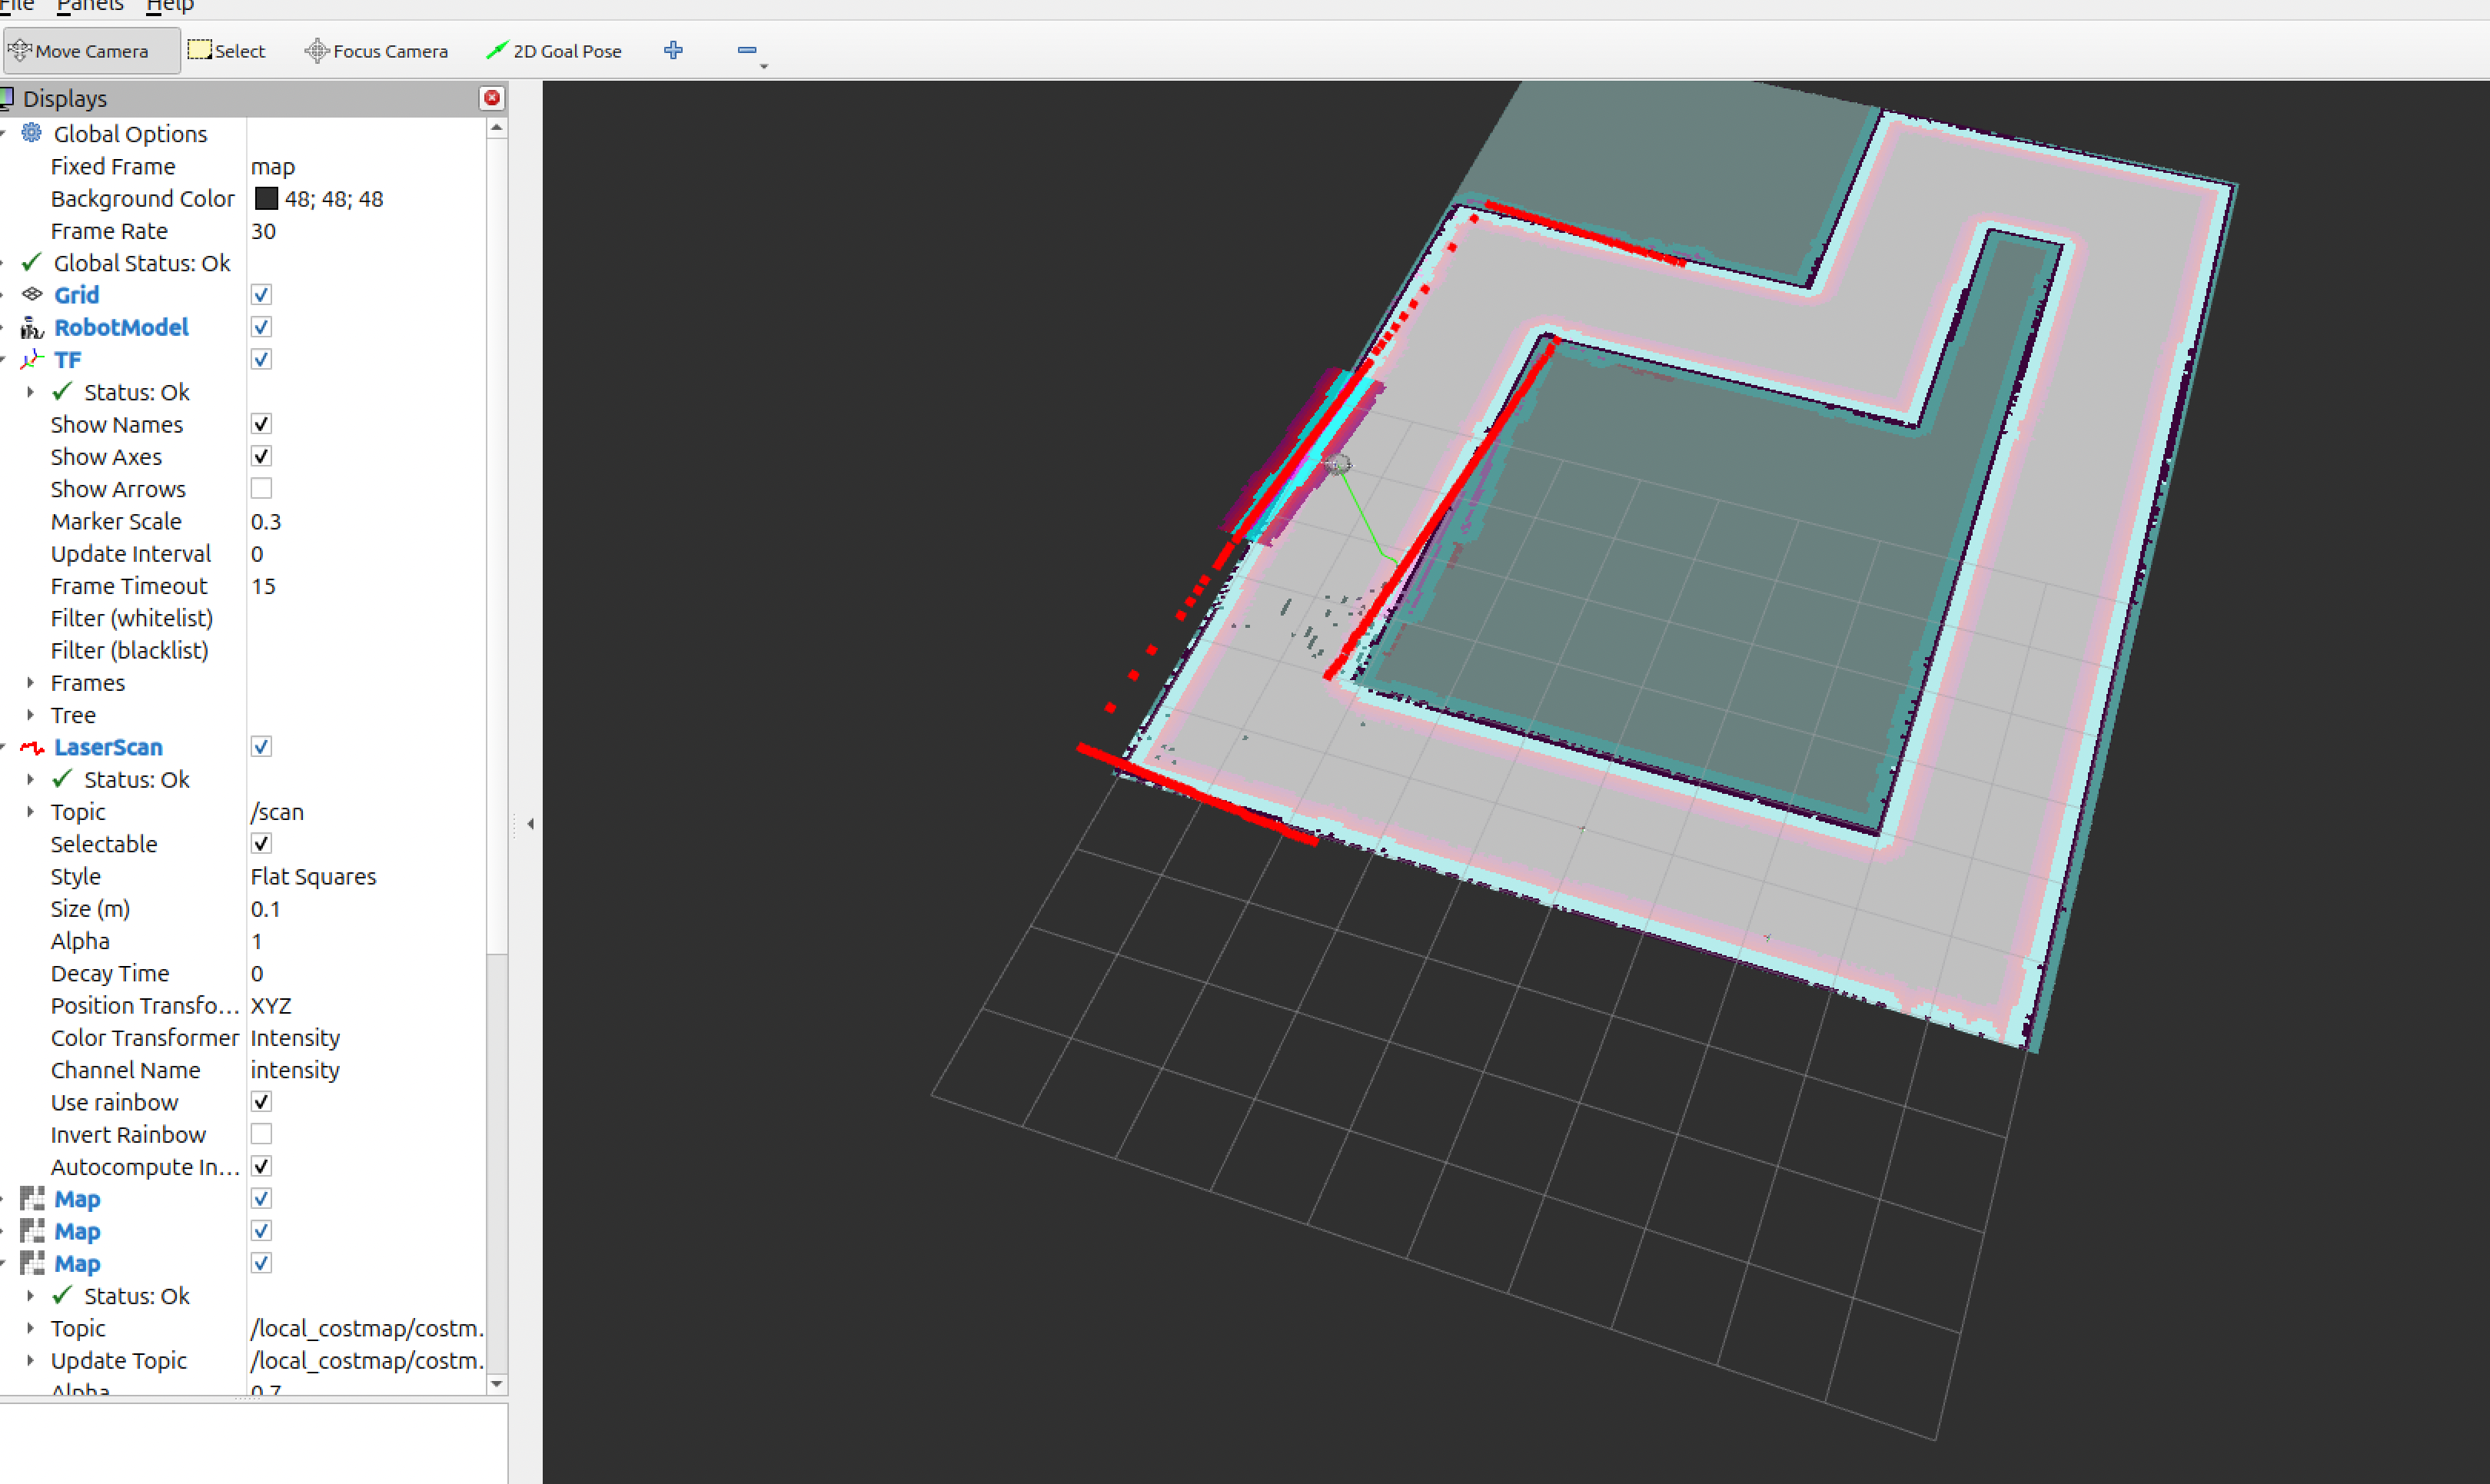
\includegraphics[width=\columnwidth]{fig/12_image.png}
        \caption{End. The whole maze is mapped, but the scan on the left does
                 not line up with the map.}
    \end{subfigure}
    \caption{The last part of the exploration.}
    \label{fig:explore2}
\end{figure}

\section{Reflection}
This was a good assignment to implement, as we learned how costmaps can be used for exploring the maze, and it was good to see it visually. Other than this, the assignment gave us a good indication of what we wanted to do for our exam project.

\end{document}
